\documentclass[11pt,a4paper]{article}
\usepackage[utf8]{inputenc}
\usepackage[spanish,es-noshorthands,es-tabla]{babel}
\usepackage{amsmath}
\usepackage{graphicx}
\usepackage[hidelinks]{hyperref}
\usepackage{bookmark}
\usepackage{titlesec}
\usepackage{fancyhdr}
\usepackage{geometry}
\usepackage{eso-pic}   % Required for background image
\usepackage{graphicx}  % Required for background image
\usepackage{caption}
\usepackage{subcaption}
\usepackage{xcolor}
\usepackage{cellspace}
\usepackage{amsmath, amssymb, booktabs}
\usepackage{tabularx}
\usepackage{array}
\renewcommand{\arraystretch}{1.3} % espacio entre filas de las tablas
\usepackage{float}
\usepackage[siunitx]{circuitikz}   % Required for circuit diagrams
\usepackage{pgfplots}
\usepackage{pgfplotstable} % Optional for importing data tables
\usepackage{tikz}
\usetikzlibrary{arrows.meta, patterns, circuits.logic.US, positioning}
\usepackage{textcomp}
\usepackage{gensymb}
\usepackage{siunitx}
\sisetup{output-decimal-marker={,}}
\usepackage{wrapfig}

\pgfplotsset{compat=1.18}
\graphicspath{{../img/}}

\newcolumntype{C}{>{\centering\arraybackslash}X}

\definecolor{darkGreen}{HTML}{4cba66}

% Page layout
\geometry{
    a4paper,
    left=2.5cm,
    right=2.5cm,
    top=0.5cm,
    bottom=3.5cm,
    includehead,
    headheight=85pt,
    footskip=1.2cm
}

% Header and Footer
\pagestyle{fancy}
\chead{
    
\includegraphics[width=0.75\paperwidth]{upct_header.png} \\[15pt]
}
\fancyfoot[C]{\thepage} % Page number

\setlength{\headheight}{85pt}
\setlength{\skip\footins}{14pt}

\setlength{\parindent}{0pt} % No indentation
\setlength{\parskip}{\baselineskip} % Space between paragraphs

\setlength{\intextsep}{25pt} % Space between text and images

\setlength\cellspacetoplimit{4pt}
\setlength\cellspacebottomlimit{4pt}

\setlength{\parskip}{10pt}  % Space between paragraphs




% Title format
\titleformat{\section}{\normalfont\Large\bfseries}{\thesection}{1em}{}

% Title spacing
\titlespacing{\section}{0pt}{10pt}{1pt} % Space between title and text
\titlespacing{\subsection}{0pt}{10pt}{1pt} % Space between subtitle and text
\begin{document}

% Title page
\newlength{\TitleSidebarWidth}
\newlength{\TitleMargin}
\newlength{\TitlePageLeftMargin}
\newlength{\TitleUpctLogoWidth}
\newlength{\TitleSchoolTextWidth}
\newlength{\TitleSchoolTextTop}
\newlength{\TitleBottomLogoWidth}
\newlength{\TitleBottomTextWidth}
\newlength{\TitleBottomBlockBottom}
\newlength{\TitleBottomLogoBottom}

\setlength{\TitleSidebarWidth}{40mm}
\setlength{\TitleMargin}{25mm}
\setlength{\TitlePageLeftMargin}{\dimexpr\TitleSidebarWidth+\TitleMargin\relax}
\setlength{\TitleUpctLogoWidth}{90mm}
\setlength{\TitleSchoolTextWidth}{34mm}
\setlength{\TitleSchoolTextTop}{12mm}
\setlength{\TitleBottomLogoWidth}{16mm}
\setlength{\TitleBottomTextWidth}{34mm}
\setlength{\TitleBottomBlockBottom}{18mm}
\setlength{\TitleBottomLogoBottom}{68mm}

\let\OriginalTitlePage\titlepage
\let\EndOriginalTitlePage\endtitlepage
\renewenvironment{titlepage}{
    \newgeometry{
        left=\TitlePageLeftMargin,
        right=\TitleMargin,
        top=\TitleMargin,
        bottom=\TitleMargin
    }
    \OriginalTitlePage
}{
    \EndOriginalTitlePage
    \restoregeometry
    \clearpage
}

\newcommand\BackgroundPic{
    \begin{tikzpicture}[remember picture, overlay]
        \node[anchor=south west, inner sep=0pt] at (current page.south west) {
            
\includegraphics[
                width=\TitleSidebarWidth,
                height=\paperheight
            ]{Contraportada-40x297.png}
        };
        \node[
            anchor=north,
            inner sep=0pt,
            align=left,
            text=white,
            text width=\TitleSchoolTextWidth,
            font=\small\bfseries,
            xshift=0.55\TitleSidebarWidth,
            yshift=-3\TitleSchoolTextTop
        ] at (current page.north west) {
            \sffamily{Escuela Técnica \\Superior\\ de Ingeniería de\\ Telecomunicación}
        };
        \node[
            anchor=center,
            inner sep=0pt,
            opacity=0.3,
            xshift=\TitleSidebarWidth
        ] at (current page.west) {
            
\includegraphics[width=\TitleUpctLogoWidth]{logo_upct_blanco_vector.png}
        };
        \node[
            anchor=south,
            inner sep=0pt,
            align=center,
            xshift=0.5\TitleSidebarWidth,
            yshift=\TitleBottomLogoBottom
        ] at (current page.south west) {
            
\includegraphics[width=\TitleBottomLogoWidth]{logo_upct.png}
        };
        \node[
            anchor=south,
            inner sep=0pt,
            align=left,
            text=white,
            text width=\TitleBottomTextWidth,
            xshift=0.55\TitleSidebarWidth,
            yshift=2.5\TitleBottomBlockBottom
        ] at (current page.south west) {
            {\sffamily\LARGE Universidad\\[-1mm]Politécnica\\[1mm]de Cartagena}
        };
    \end{tikzpicture}
}
% End title page

\begin{titlepage}

    % Background image
    \AddToShipoutPicture*{\BackgroundPic}

    % 
\includegraphics[width=0.8\paperwidth]{upct_header.png}

    \centering
    \vspace*{0cm}
    \Huge{\textbf{UNIVERSIDAD POLITÉCNICA DE CARTAGENA}}

    \vspace{0.5cm}
    \Huge{Escuela Técnica Superior de Ingeniería de Telecomunicación}

    \vspace{2cm}
    \LARGE{\textbf{Mejora de la resolución angular de un radar UWB mediante arrays virtuales MIMO diseñados con un sistema de orquestación de agentes de IA}}

    \vspace{2cm}
    \LARGE{\textbf{Trabajo Fin de Estudios}}

    \vspace{0.3cm}
    \Large{GRADO EN INGENIERÍA EN SISTEMAS \\ 
    DE TELECOMUNICACIÓN}

    \vfill
    \large{\textbf{Autor:}} Luis Carretero López \\
    \vspace{0.2cm}
    \large{\textbf{Directores:}} José Luis Gómez Tornero y Manuel Saez Martínez 

    \vspace{1cm}
    \large{\today}
\end{titlepage}


% Resumen en español
\newpage
\section*{Resumen}
\addcontentsline{toc}{section}{Resumen}
Este Trabajo de Fin de Estudios aborda el diseño de un elemento radiante para el canal~9 de
IEEE 802.15.4z, con un ancho de banda de \SI{499.2}{MHz} centrado en \SI{7.9872}{GHz}, y su
integración en un array lineal de cinco elementos, con el objetivo de mejorar la resolución
angular de un radar UWB de detección de personas. El SoC del radar dispone de dos puertos de radiofrecuencia (uno de
transmisión-recepción y otro solo de recepción), por lo que el array se opera como un array virtual MIMO por multiplexación
en el tiempo.

El elemento se diseña sobre un sustrato FR-4 provisional, se evalúa con openEMS, un solver FDTD
libre, y se valida con Ansys HFSS. Los candidatos se juzgan por su adaptación en toda la banda,
la eficiencia de radiación, la ganancia realizada y el rizado del retardo de grupo radiado. El
array de cinco elementos se simula en HFSS; su respuesta como array virtual se obtiene sumando de
forma coherente los diagramas embebidos exportados, y la separación entre elementos se barre de
forma paramétrica.

El diseño sigue un ciclo iterativo apoyado en un sistema de orquestación de agentes de
inteligencia artificial basado en modelos de Anthropic. Un orquestador (Claude Opus 5.5) reparte
las tareas entre subagentes especializados (Claude Sonnet 5.5) en diseño RF, modelado
electromagnético y auditoría; un revisor (Claude Fable~5.2) revisa el diseño antes de simularlo
en HFSS. Otros subagentes se encargan de tareas más ligeras, como la
representación gráfica de los datos y la revisión del código.

% Abstract in English
\newpage
\section*{Abstract}
\addcontentsline{toc}{section}{Abstract}
{\sisetup{output-decimal-marker={.}}This Bachelor's Thesis addresses the design of a radiating element for channel 9 of IEEE
802.15.4z, with a bandwidth of \SI{499.2}{MHz} centred at \SI{7.9872}{GHz}, and its integration
into a five-element linear array, aiming to improve the angular resolution of a UWB radar for
person detection. The radar SoC has two RF ports (one transmit-receive and one receive-only), so the array operates as a virtual MIMO
array through time-division multiplexing.

The element is designed on a provisional FR-4 substrate, evaluated with openEMS, an open-source
FDTD solver, and validated with Ansys HFSS. Candidates are assessed by their matching over the
whole band, radiation efficiency, realised gain and radiated group-delay ripple. The five-element
array is simulated in HFSS; its virtual-array response is obtained by coherently summing the
exported embedded element patterns, and the element spacing is swept parametrically.

The design follows an iterative cycle supported by an AI agent orchestration system based on
Anthropic models: an orchestrator (Claude Opus 5.5) distributes tasks among specialised
subagents (Claude Sonnet 5.5) for RF design, electromagnetic modelling and independent auditing;
a design reviewer (Claude Fable~5.2) reviews the design before its HFSS simulation. Other
subagents handle lighter tasks, such as plotting the data and reviewing the code.}

% Declaración de uso de inteligencia artificial
\newpage
\section*{Declaración de uso de inteligencia artificial}
\addcontentsline{toc}{section}{Declaración de uso de inteligencia artificial}
En este Trabajo de Fin de Estudios se han utilizado herramientas de inteligencia artificial
generativa, en concreto modelos de lenguaje de Anthropic ejecutados en el entorno Claude Code. Su
uso ha sido de dos tipos.

\paragraph{Como parte de la metodología del trabajo.} El sistema de orquestación de agentes descrito
en la Sección~\ref{sec:agentes_arquitectura} es uno de los objetos de estudio del trabajo. Un
orquestador (Claude Opus 5.5) y varios subagentes (Claude Sonnet 5.5) propusieron geometrías,
prepararon y ejecutaron las simulaciones de openEMS, generaron los \textit{scripts} de HFSS,
analizaron los resultados, generaron las gráficas a partir de los ficheros de simulación y
auditaron los resultados y el código. Un revisor (Claude Fable~5.2) revisó los diseños antes de
simularlos en HFSS. Su funcionamiento, su coste y sus limitaciones se describen y evalúan en la
memoria.

\paragraph{Como apoyo en la redacción de la memoria.} Se han utilizado Claude Haiku 5.5 y Claude
Opus 5.5 para elaborar borradores de algunas secciones, comprobar las cifras del texto frente a los
datos de simulación, preparar figuras y tablas a partir de los resultados y revisar el estilo y el
formato del documento.

\paragraph{Supervisión y responsabilidad.} El autor definió los objetivos y las restricciones del
trabajo, tomó las decisiones de diseño, ejecutó las simulaciones de HFSS en su equipo y revisó el
contenido generado con ayuda de estas herramientas. Todas las cifras de la memoria proceden de
simulaciones de openEMS o de HFSS; ningún resultado se ha obtenido de un modelo de lenguaje sin una
simulación que lo respalde. Los informes de cada iteración, los datos de simulación y el historial
de cambios se conservan en el repositorio del proyecto. El autor asume la plena responsabilidad del
contenido de este documento.

% Table of contents
\newpage
\tableofcontents

\newpage
\listoffigures

\newpage
\listoftables

\newpage
\section{Introducción}\label{sec:introduccion}
Esta sección sitúa el trabajo en el contexto de los radares UWB de corto alcance, presenta el
array de referencia del que se parte, formula el problema técnico y enumera los objetivos del TFE.

\subsection{Contexto}
Los transceptores IEEE 802.15.4z emplean canales de banda ultraancha, o UWB
(\textit{Ultra-Wideband}), de $B = \SI{499.2}{MHz}$ \cite{ieee802154z2020}. Además de medir
distancias entre dispositivos, los chips que exponen la respuesta al impulso del canal (CIR,
\textit{Channel Impulse Response}) permiten construir radares de corto alcance
\cite{cheraghinia2024uwbradar}. Con una sola antena, un radar de este tipo separa dos objetivos
solo por su distancia, y lo consigue cuando sus rangos difieren más de $c/2B \approx \SI{0.3}{m}$.
Para localizar un objetivo en azimut hace falta una dimensión espacial, que aporta un array de
antenas: la diferencia de fase entre elementos codifica la dirección de llegada del eco
\cite{vantrees2002array}.

Este TFE se enmarca en un radar UWB para la detección de personas, desarrollado en colaboración
con la empresa AED Vantage S.L. El radar opera en el canal~9 del estándar, centrado en
\SI{7.9872}{GHz} y con una banda de \SI{7.7376}{GHz} a \SI{8.2368}{GHz}.

\subsection{Motivación}
El SoC que procesa las señales del radar dispone de solo dos puertos de radiofrecuencia (uno de
transmisión-recepción y otro solo de recepción). Esta limitación impide adquirir de forma simultánea las señales de todos los
elementos de un array. Para superarla se recurre a un array virtual MIMO
(\textit{Multiple Input Multiple Output}) por multiplexación en el tiempo (TDM): una matriz de
conmutación asigna en cada intervalo los puertos del SoC a los elementos del array, y el
sistema recorre así los pares transmisor-receptor de cada adquisición (Sección~\ref{sec:array_mimo}). Cada par equivale a un elemento virtual
situado en el punto medio entre ambas antenas, de modo que el array virtual dispone de más
posiciones y de más apertura eléctrica que el físico.

En el artículo «Design of Virtual Phased Arrays for Ultrawideband Localization» \cite{carretero2027vpa},
los investigadores analizan un array virtual TDM-MIMO de este tipo. Su array consta de cuatro parches apilados con cavidad, idénticos y con
la misma orientación, dispuestos en línea con una separación de \SI{13.5}{mm} ($0{,}35\lambda$ a
$0{,}37\lambda$ en la banda) sobre una placa FR-4 de $57{,}9 \times \SI{36}{mm}$. El elemento
cubre los canales~9, 10 y~12. Su esquema incluye además los pares monoestáticos, en los que un
mismo elemento transmite y recibe, y con ellos los cuatro elementos generan siete posiciones
virtuales; con una
separación de $0{,}36\lambda$ el haz transversal se estrecha de \SI{36.9}{\degree}, en recepción
pura, a \SI{24.0}{\degree} con el array virtual. Este TFE toma esa disposición y ese ancho de haz
como referencia de partida.

El ancho de haz de \SI{24}{\degree} limita la capacidad del radar para separar dos personas
próximas en azimut dentro de una misma celda de rango. Reducirlo exige actuar sobre el elemento
radiante y sobre la geometría del array. El elemento fija la adaptación, la eficiencia, la
ganancia y el retardo de grupo, y la geometría fija la apertura virtual y la aparición de lóbulos
de rejilla.

\subsection{Problema que se quiere resolver}
El problema técnico consiste en mejorar la resolución angular del array virtual de referencia
manteniendo la restricción de dos puertos RF. La solución pasa por dos tareas encadenadas.

La primera es diseñar un elemento radiante nuevo para el canal~9. Este TFE estudia el elemento
solo en ese canal, a diferencia del array de referencia, que cubre los canales~9, 10 y~12. El
elemento debe presentar $|S_{11}| < \SI{-10}{dB}$ en toda la banda de \SI{499.2}{MHz} con
referencia a \SI{50}{\ohm}, y además una eficiencia de radiación y una ganancia realizada
suficientes y un retardo de grupo con poco rizado, porque el rizado del retardo de grupo genera
falsos objetivos en rango \cite{carretero2027vpa}. Un mínimo puntual de $|S_{11}|$ no cumple el
requisito: la adaptación debe cubrir la banda completa.

La segunda tarea es integrar el elemento en un array lineal de cinco antenas, una más que el
array de referencia, para aumentar la apertura del array virtual; obtener la respuesta del array
virtual MIMO, y buscar la separación entre elementos que estreche el haz sin introducir lóbulos de
rejilla.

El diseño de antenas UWB exige muchas iteraciones de geometría, simulación electromagnética y
análisis. Para acelerar ese ciclo, este TFE construye un sistema de agentes de inteligencia
artificial, basado en modelos de Anthropic, que propone geometrías, las simula con openEMS y
analiza los resultados de forma autónoma. Los diseños prometedores se validan después en Ansys
HFSS.

\subsection{Objetivos}
El objetivo general del TFE es mejorar la resolución angular del array virtual MIMO de referencia
mediante el diseño de un nuevo elemento radiante para el canal~9 y la optimización de la
geometría del array. Para ello se plantean los siguientes objetivos específicos:

\begin{itemize}
    \item Diseñar un sistema de orquestación de agentes de IA que reparta las tareas del diseño
    de antenas (investigación de topologías, modelado electromagnético y análisis de resultados)
    entre modelos de Anthropic según su complejidad, sobre un entorno Python con openEMS y
    \textit{skills} especializadas en antenas y RF.
    \item Diseñar de forma iterativa un elemento radiante para el canal~9 con
    $|S_{11}| < \SI{-10}{dB}$ en toda la banda, buena eficiencia y ganancia realizada y bajo
    rizado del retardo de grupo, siguiendo el ciclo de simulación en openEMS, análisis,
    refinamiento y validación en HFSS.
    \item Simular en HFSS un array lineal de cinco elementos, exportar los diagramas de radiación de
    cada puerto y combinarlos de forma coherente según las configuraciones MIMO para obtener la
    respuesta del array virtual.
    \item Barrer de forma paramétrica la separación entre elementos para determinar la separación
    óptima y comparar la resolución angular obtenida con la del array de referencia.
\end{itemize}

\section{Estado del arte y fundamentos}\label{sec:estado_del_arte}
Esta sección reúne los fundamentos que sostienen el trabajo: la capa física UWB del canal~9, los
parámetros que caracterizan una antena para pulsos UWB, las técnicas de ensanchamiento de banda en
antenas de parche, la teoría de arrays lineales, el array virtual MIMO, los métodos de simulación
electromagnética y el uso de agentes de inteligencia artificial en el diseño de ingeniería.

\subsection{Tecnología UWB y canal 9 de IEEE 802.15.4z}\label{sec:uwb}
La FCC define una señal UWB como aquella que ocupa al menos \SI{500}{MHz} o un ancho de banda
fraccional de al menos el 20\,\% \cite{fcc2002uwb}. La capa física HRP
(\textit{High Rate Pulse repetition frequency}) de IEEE 802.15.4 transmite pulsos cuya duración es
del orden de $1/B$, y la enmienda 802.15.4z añade mecanismos para medir distancias de forma
segura \cite{ieee802154z2020}. Coppens \textit{et al.} revisan cómo se reparten estos canales
entre el IEEE, el consorcio FiRa y los fabricantes de chips \cite{coppens2022uwb}.

La Tabla~\ref{tab:canal9} resume los parámetros del canal~9, el único que estudia este TFE. Con
$B = \SI{499.2}{MHz}$, los pulsos duran unos \SI{2}{ns} y la resolución en rango vale
\begin{equation}
    \Delta R = \frac{c}{2B} \approx \SI{0.30}{m}.
    \label{eq:resolucion_rango}
\end{equation}
Esta resolución temporal, junto con el bajo coste de los chips, explica el interés reciente por
los radares UWB de corto alcance para detección de personas, monitorización de constantes vitales
y localización en interiores \cite{cheraghinia2024uwbradar}.

\begin{table}[H]
    \centering
    \caption{Parámetros del canal~9 de IEEE 802.15.4z.}
    \label{tab:canal9}
    \begin{tabular}{lc}
        \toprule
        Parámetro & Valor \\
        \midrule
        Frecuencia central $f_0$ & \SI{7.9872}{GHz} \\
        Banda & \SIrange{7.7376}{8.2368}{GHz} \\
        Ancho de banda $B$ & \SI{499.2}{MHz} \\
        Ancho de banda fraccional & 6,25\,\% \\
        Longitud de onda en el vacío $\lambda_0$ & \SI{37.5}{mm} \\
        Resolución en rango $c/2B$ & \SI{0.30}{m} \\
        \bottomrule
    \end{tabular}
\end{table}

\subsection{Antenas para pulsos UWB}\label{sec:antenas_uwb}
En un sistema de banda estrecha basta con caracterizar la antena a la frecuencia central. En
un sistema de pulsos la antena actúa como un filtro: cualquier variación de su respuesta con la
frecuencia deforma el pulso radiado. Wiesbeck, Adamiuk y Sturm describen la antena UWB como un
sistema lineal con una función de transferencia dependiente de la dirección y de la frecuencia, y
proponen evaluarla tanto en frecuencia como en tiempo \cite{wiesbeck2009uwb}. Este TFE emplea
los parámetros siguientes.

\paragraph{Adaptación.} El coeficiente de reflexión en el puerto de alimentación,
\begin{equation}
    S_{11} = \frac{Z_\mathrm{in} - Z_0}{Z_\mathrm{in} + Z_0}, \qquad Z_0 = \SI{50}{\ohm},
    \label{eq:s11}
\end{equation}
mide la fracción de la onda incidente que vuelve al transceptor \cite{pozar2012microwave}. El
criterio habitual exige $|S_{11}| < \SI{-10}{dB}$, que equivale a reflejar menos del 10\,\% de la
potencia. Para un pulso, el criterio debe cumplirse en toda la banda: un mínimo estrecho y
profundo en $f_0$ deja los extremos del canal desadaptados.

El límite de Bode-Fano acota el ancho de banda alcanzable para una carga resonante de factor de
calidad $Q$ dado \cite{fano1950bode}. Una antena de parche delgada presenta un $Q$ alto, y por eso
su ancho de banda de adaptación natural no suele cubrir los \SI{499.2}{MHz} del canal.

\paragraph{Eficiencia y ganancia realizada.} La eficiencia de radiación $e_\mathrm{rad}$ compara
la potencia radiada con la aceptada por la antena, y descuenta las pérdidas en el dieléctrico y en
el metal. La ganancia realizada incorpora además la desadaptación \cite{balanis2016antenna}:
\begin{equation}
    G_\mathrm{real}(\theta,\phi) = \left(1 - |S_{11}|^2\right) e_\mathrm{rad}\, D(\theta,\phi),
    \label{eq:ganancia_realizada}
\end{equation}
donde $D$ es la directividad. La ganancia realizada fija la relación señal a ruido del eco en cada
dirección.

\paragraph{Retardo de grupo.} El retardo de grupo radiado en la dirección $(\theta,\phi)$ se
obtiene de la fase $\varphi$ de la función de transferencia de la antena:
\begin{equation}
    \tau_g(f;\theta,\phi) = -\frac{1}{2\pi}\frac{\partial \varphi(f;\theta,\phi)}{\partial f}.
    \label{eq:retardo_grupo}
\end{equation}
Un retardo de grupo constante desplaza el pulso sin deformarlo. Su rizado con la frecuencia
ensancha el pulso y crea lóbulos secundarios en rango \cite{wiesbeck2009uwb}. En un radar el eco
atraviesa la antena dos veces, de modo que el efecto se duplica; en el array de referencia el
rizado del retardo de grupo genera falsos objetivos en rango \cite{carretero2027vpa}. La
derivada de la fase de $S_{11}$ no equivale al retardo de grupo radiado: describe la reflexión
en el puerto, no el campo lejano.

\subsection{Antenas de parche y ensanchamiento de banda}\label{sec:parches}
Una antena de parche microstrip consta de una lámina metálica sobre un sustrato dieléctrico con
plano de masa. En el modo fundamental TM$_{10}$ el parche resuena cuando su longitud vale
aproximadamente media longitud de onda en el dieléctrico \cite{balanis2016antenna}:
\begin{equation}
    L \approx \frac{c}{2 f_0 \sqrt{\varepsilon_\mathrm{eff}}} - 2\Delta L,
    \label{eq:longitud_parche}
\end{equation}
donde $\varepsilon_\mathrm{eff}$ es la permitividad efectiva y $\Delta L$ la extensión por los
campos de borde. El parche es compacto, plano y fácil de fabricar en la misma placa que el
transceptor, pero su ancho de banda es estrecho, del orden de pocas unidades por ciento para
sustratos delgados.

La literatura recoge varias técnicas para ensanchar la banda:
\begin{itemize}
    \item \textbf{Sustratos más gruesos y de menor permitividad}, que reducen el $Q$ de la
    cavidad a costa de excitar ondas de superficie y aumentar la inductancia de la alimentación
    \cite{balanis2016antenna}.
    \item \textbf{Ranuras en el parche}. La ranura en U de Huynh y Lee introduce una segunda
    resonancia próxima a la del parche y multiplica el ancho de banda del parche con
    alimentación por sonda \cite{huynh1995uslot}.
    \item \textbf{Parches apilados}. Un parche parásito sobre el excitado añade una resonancia
    acoplada. El elemento del array de referencia combina un parche excitado, un parche parásito
    enterrado y ranuras de impedancia escalonada dentro de una cavidad, y obtiene una escalera de
    cuatro resonadores acoplados que cubre los canales 9, 10 y 12 \cite{carretero2027vpa}.
    \item \textbf{Cavidades y vallados de vías}, que confinan el campo, reducen las ondas de
    superficie y el acoplamiento entre elementos vecinos de un array \cite{carretero2027vpa}.
\end{itemize}
Este TFE parte de estas familias para explorar geometrías candidatas para el canal~9: el parche
rectangular y el parche con ranura en U, al que más adelante se añade un parche parásito enterrado.

\subsection{Arrays lineales y resolución angular}\label{sec:arrays}
Un array lineal de $N$ elementos idénticos situados en $x_n$ a lo largo del eje $x$ produce un
diagrama de radiación que, en ausencia de acoplamiento, factoriza en el diagrama del elemento y
el factor de array \cite{balanis2016antenna, vantrees2002array}:
\begin{equation}
    AF(\alpha) = \sum_{n=0}^{N-1} w_n\, e^{\,j k x_n \sin\alpha},
    \qquad k = \frac{2\pi}{\lambda},
    \label{eq:factor_array}
\end{equation}
donde $\alpha$ es el ángulo de azimut medido desde la normal al array y $w_n$ los pesos
complejos. Con pesos uniformes y separación $d$, el ancho de haz a \SI{-3}{dB} en la dirección
transversal se aproxima, para $N$ grande, por
\begin{equation}
    \theta_{3\,\mathrm{dB}} \approx 0{,}886\,\frac{\lambda}{N d}\ \ \mathrm{rad}.
    \label{eq:ancho_haz}
\end{equation}
La resolución angular depende, por tanto, de la apertura $Nd$ medida en longitudes de onda. Dos
objetivos en la misma celda de rango se separan en azimut si su diferencia angular supera, de
forma aproximada, el ancho del haz.

Aumentar $d$ estrecha el haz, pero si la separación supera
\begin{equation}
    d < \frac{\lambda}{1 + |\sin\alpha_\mathrm{max}|},
    \label{eq:lobulos_rejilla}
\end{equation}
aparecen lóbulos de rejilla al apuntar a $\alpha_\mathrm{max}$, réplicas del haz principal que
producen ambigüedad angular \cite{mailloux2005phased}. Para un barrido de $\pm\SI{90}{\degree}$ la
condición exige $d < \lambda/2$. La separación óptima resulta así de un compromiso entre
resolución y ambigüedad, y además depende del tamaño físico del elemento, que fija la separación
mínima realizable.

La factorización de la ecuación~\eqref{eq:factor_array} supone elementos idénticos y aislados. En
un array real, el acoplamiento mutuo y el borde finito de la placa hacen que cada elemento radie
un diagrama distinto. Pozar define el diagrama embebido, o \textit{active element pattern}, como
el diagrama de un elemento excitado con el resto de puertos cargados con \SI{50}{\ohm}
\cite{pozar1994active}. Este TFE trabaja con los diagramas embebidos que exporta HFSS para cada
puerto, y no con un factor de array ideal.

\subsection{Radar MIMO y array virtual}\label{sec:mimo}
En un radar MIMO con antenas colocalizadas, cada transmisor emite una forma de onda separable en
recepción, y el receptor procesa cada par transmisor-receptor por separado \cite{li2007mimo}. En
campo lejano, el eco de un objetivo en la dirección $\alpha$ recorre el camino de ida desde
$x_t$ y el de vuelta hasta $x_r$, y acumula el desfase
\begin{equation}
    \Phi_{tr}(\alpha) = k\,(x_t + x_r)\sin\alpha = \frac{4\pi}{\lambda}\, v_{tr} \sin\alpha,
    \qquad
    v_{tr} = \frac{x_t + x_r}{2},
    \label{eq:posicion_virtual}
\end{equation}
siendo el mismo que mediría un radar monoestático situado en el punto medio $v_{tr}$ del par.
En este caso, el desfase crece con $4\pi/\lambda$ en lugar de $2\pi/\lambda$
por el doble recorrido. Una extensión de las posiciones virtuales $L_v$ equivale, por tanto, a
una apertura eléctrica de $2L_v$ en un array convencional de recepción, y la
ecuación~\eqref{eq:ancho_haz} se aplica sustituyendo $Nd$ por esa apertura equivalente. El análisis de antenas en HFSS escribe la misma fase como
$k\,(x_t+x_r)$, sin dividir por dos, y sitúa el elemento virtual en $x_t+x_r$. Ambas formulaciones son
equivalentes, porque $k\,(x_t+x_r) = (4\pi/\lambda)\,v_{tr}$: solo cambia la escala con que se numera la
posición, y por eso los listados del análisis de antenas expresan las posiciones en unidades de $x_t+x_r$,
el doble de $v_{tr}$.

Cuando el hardware dispone de pocos puertos, la separación entre formas de onda se consigue por
multiplexación en el tiempo (TDM): una matriz de conmutadores activa en cada intervalo un único
par. El array de referencia de este TFE sigue este esquema con un solo transceptor de dos puertos
y una matriz de conmutación de $2 \times 4$ \cite{carretero2027vpa}. Con cuatro elementos en
$0, d, 2d, 3d$, los diez pares distintos, monoestáticos incluidos, ocupan siete posiciones
virtuales, de $0$ a $3d$ en pasos de $d/2$, con multiplicidades $1, 1, 2, 2, 2, 1, 1$. Por el
doble recorrido, la apertura eléctrica equivale a $6d$, el doble de la física, y con
$d = 0{,}36\lambda$ el haz transversal pasa de \SI{36.9}{\degree} en recepción pura a
\SI{24.0}{\degree} \cite{carretero2027vpa}. La multiplicidad no uniforme actúa además como una
ventana que reduce los lóbulos secundarios.

El esquema TDM tiene dos limitaciones que condicionan el diseño. La primera es temporal: un
objetivo en movimiento cambia de fase entre intervalos, lo que sesga el azimut si el orden de los
intervalos no se elige con cuidado. La segunda es electromagnética: la suma coherente supone que
los elementos son idénticos, y las diferencias entre diagramas embebidos sesgan el azimut y elevan
los lóbulos secundarios \cite{carretero2027vpa}. Por eso el elemento y el array se diseñan aquí
juntos.

\subsection{Simulación electromagnética}\label{sec:simulacion}
Ninguna expresión cerrada predice con exactitud la impedancia, el diagrama y el retardo de grupo
de un parche con ranuras dentro de un array. El diseño requiere resolver numéricamente las
ecuaciones de Maxwell. Este TFE usa dos métodos complementarios.

\paragraph{FDTD.} El método de diferencias finitas en el dominio del tiempo discretiza el espacio
en la celda de Yee, con las componentes del campo eléctrico y magnético intercaladas en espacio y
tiempo, y avanza la solución con un esquema explícito \cite{yee1966numerical, taflove2005fdtd}.
Una sola simulación excitada con un pulso de banda ancha devuelve, mediante la transformada de
Fourier, la respuesta en toda la banda. La estabilidad impone un paso temporal ligado a la celda
más pequeña (condición de Courant), de modo que los detalles finos de la geometría encarecen la
simulación. openEMS es una implementación libre de FDTD con interfaz en Python y MATLAB
\cite{liebig2013openems}, que permite generar y simular geometrías desde un programa.

\paragraph{FEM.} El método de elementos finitos resuelve el problema en el dominio de la
frecuencia sobre una malla de tetraedros que se adapta a la geometría \cite{jin2014fem}. Ansys
HFSS refina la malla de forma adaptativa hasta que la variación de los parámetros $S$ entre pasadas
cae por debajo de un umbral, y es una referencia habitual en el diseño de antenas.

FDTD y FEM discretizan el problema de forma distinta, y sus resultados sobre la misma geometría no
coinciden exactamente. En este trabajo openEMS actúa como herramienta de exploración, libre y
automatizable, y HFSS como herramienta de validación de los candidatos y de simulación del array.

\subsection{Agentes de inteligencia artificial en el diseño de ingeniería}\label{sec:agentes}
La optimización automática de antenas tiene una larga trayectoria. Los algoritmos genéticos
\cite{haupt1995genetic} y la optimización por enjambre de partículas \cite{robinson2004pso}
acoplan un optimizador con un simulador electromagnético y exploran un espacio de parámetros
definido de antemano. Estos métodos ajustan dimensiones de una topología fija, pero no proponen
topologías nuevas ni interpretan por qué un diseño falla.

Los modelos de lenguaje de gran tamaño han abierto otra vía. Un agente combina un modelo de
lenguaje con herramientas externas y alterna razonamiento y acciones: lee resultados, decide el
siguiente paso y ejecuta código \cite{yao2023react}. Anthropic describe varios patrones de
composición de agentes, entre ellos el de orquestador y trabajadores, en el que un modelo central
divide la tarea, la delega en subagentes especializados y sintetiza sus resultados
\cite{anthropic2024agents}. Este patrón permite asignar cada subtarea al modelo más adecuado según
su complejidad y su coste.

Aplicado al diseño de antenas, un sistema de agentes puede investigar topologías en la
literatura, escribir el modelo de simulación, ejecutar el solver, interpretar $S_{11}$, la
ganancia y el retardo de grupo y proponer el siguiente refinamiento. Este TFE construye un sistema
de este tipo sobre openEMS y lo integra con la validación en HFSS. La sección~\ref{sec:metodologia}
describe su arquitectura.

\section{Metodología}\label{sec:metodologia}
Esta sección describe el procedimiento seguido para pasar de la especificación del canal~9 a la
respuesta del array virtual: la arquitectura del sistema de agentes, el modelado y la evaluación
del elemento en openEMS, el ciclo de refinamiento y validación en HFSS, la simulación del array y
su combinación MIMO, y el barrido de la separación entre elementos.

\subsection{Visión general del flujo de trabajo}\label{sec:flujo}
La Figura~\ref{fig:flujo} resume el flujo. El trabajo se divide en dos etapas. En la primera, el
sistema de agentes propone geometrías de elemento, las simula en openEMS y analiza los resultados,
y los candidatos que se acercan al objetivo pasan a HFSS para su validación. En la segunda, el
elemento validado se integra en un array lineal de cinco elementos en HFSS, se exportan sus diagramas
embebidos y un programa en Python los combina según las configuraciones MIMO para obtener la
respuesta del array virtual. Un barrido paramétrico de la separación entre elementos cierra el
estudio.

\begin{figure}[H]
    \centering
    \begin{tikzpicture}[
        node distance=7mm and 13mm,
        caja/.style={draw, rounded corners=2pt, align=center, minimum height=9mm,
                     text width=29mm, font=\small},
        flecha/.style={-{Stealth[length=2mm]}, thick}
    ]
        \node[caja] (inv) {Investigación de topologías\\(agente RF)};
        \node[caja, right=of inv] (oems) {Simulación del elemento\\en openEMS};
        \node[caja, right=of oems] (ana) {Análisis de resultados\\y refinamiento};
        \node[caja, below=of ana] (hfss) {Validación del elemento\\en HFSS};
        \node[caja, left=of hfss] (array) {Array de 5 elementos\\en HFSS};
        \node[caja, left=of array] (mimo) {Suma\\coherente MIMO\\y barrido de $d$};
        \draw[flecha] (inv) -- (oems);
        \draw[flecha] (oems) -- (ana);
        \draw[flecha] (ana.north) -- ++(0,5mm) -| node[pos=0.25, above, font=\scriptsize]
            {nueva iteración} (oems.north);
        \draw[flecha] (ana) -- node[right, font=\scriptsize, align=left]
            {candidato\\prometedor} (hfss);
        \draw[flecha] (hfss) -- node[above, font=\scriptsize] {cumple} (array);
        \draw[flecha] (array) -- (mimo);
    \end{tikzpicture}
    \caption{Flujo de trabajo del TFE, desde la investigación de topologías hasta la respuesta
    del array virtual.}
    \label{fig:flujo}
\end{figure}

\subsection{Sistema de orquestación de agentes}\label{sec:agentes_arquitectura}
El sistema sigue el patrón de orquestador y trabajadores descrito en la
Sección~\ref{sec:agentes}. Se ejecuta sobre Claude Code, el entorno de agentes de Anthropic, en
un repositorio de Git que contiene el código de las geometrías, los modelos de simulación, los
resultados y el estado de la campaña. Cada función del proyecto se asigna a un modelo según su
complejidad, como recoge la Tabla~\ref{tab:agentes}. El orquestador trabaja con un esfuerzo de
razonamiento medio, y los subagentes con un esfuerzo alto. El modelo más capaz y más costoso,
Fable~5.2, actúa como revisor de diseño: revisa cada diseño concreto antes de simularlo en HFSS,
una vez que se confirma esa simulación, porque un error de modelado cuesta allí más tiempo de
cálculo.

\begin{table}[H]
    \centering
    \caption{Agentes del sistema, modelo asignado y función.}
    \label{tab:agentes}
    \begin{tabularx}{\textwidth}{l l X}
        \toprule
        Agente & Modelo & Función \\
        \midrule
        Orquestador & Claude Opus 5.5 & Lee el estado de la campaña, elige la siguiente mejora,
        reparte el trabajo entre subagentes, decide si se cumple el objetivo y registra la ronda. \\
        Diseñador RF & Claude Sonnet 5.5 & Investiga topologías y propone geometría, sustrato,
        ranuras y alimentación. No ejecuta simulaciones. \\
        Especialista EM & Claude Sonnet 5.5 & Construye el modelo de openEMS (puerto, malla y
        contornos), estima los recursos y ejecuta la simulación autorizada. \\
        Validador & Claude Sonnet 5.5 & Audita de forma independiente unidades, banda, puerto,
        malla, convergencia y trazabilidad. No puede modificar ficheros. \\
        Revisor de diseño & Claude Fable~5.2 & Revisa el diseño concreto que se va a simular en
        HFSS (geometría, puertos, contornos, configuración del solver y fabricabilidad), diagnostica
        los resultados en los puntos de decisión y devuelve correcciones dirigidas al diseñador RF
        y al especialista EM. No puede modificar ficheros. \\
        Generador de gráficas & Claude Sonnet 5.5 & Prepara los datos y las gráficas de resultados a
        partir de los ficheros de simulación. No modifica los resultados. \\
        Auditor de código & Claude Sonnet 5.5 & Revisa los cambios de código (generadores de
        HFSS, exportadores, análisis y pruebas) antes de guardarlos. No puede modificar ficheros. \\
        \bottomrule
    \end{tabularx}
\end{table}

Los subagentes disponen de \textit{skills} especializadas en simulación con openEMS, líneas de
transmisión, adaptación de impedancias y diseño RF, que les aportan procedimientos y
comprobaciones de dominio. El orquestador puede lanzar como máximo tres subagentes a la vez, y
lanza en paralelo al diseñador RF y al especialista EM solo cuando sus tareas son independientes.
Cada subagente escribe únicamente los ficheros que el orquestador le asigna.

\paragraph{Rondas.} El sistema trabaja por rondas. En cada ronda el orquestador:
\begin{enumerate}
    \item sincroniza el repositorio, comprueba el estado de la campaña y reserva la ronda con un
    cerrojo para evitar dos rondas simultáneas;
    \item comprueba que el solver funciona y anota su versión;
    \item elige una sola mejora justificada a partir de las rondas anteriores, sin repetir
    candidatos ni sobrescribir resultados, y registra antes de simular una hipótesis con su
    regla de decisión;
    \item delega la geometría y el modelo, y autoriza como máximo una simulación FDTD;
    \item encarga al validador la auditoría de los resultados;
    \item escribe un informe de la ronda, actualiza el estado de la campaña y guarda todo en el
    repositorio.
\end{enumerate}
Una rutina programada en la nube lanza las rondas de forma periódica, con un contador y un número
máximo de rondas fijado. La campaña se detiene sola cuando aparece un candidato
listo para HFSS, cuando falta el solver, cuando el validador bloquea un resultado o cuando hace
falta una decisión humana.

\paragraph{Reglas de evidencia.} Un modelo de lenguaje puede presentar como resultado una
estimación que nunca se ha simulado. Para evitarlo, cada diseño lleva un estado que refleja la
procedencia real de sus datos:
\begin{itemize}
    \item \texttt{GEOMETRY\_ONLY}: geometría y estimaciones analíticas, sin parámetros
    electromagnéticos;
    \item \texttt{EM\_SIMULATED}: simulado en openEMS, con datos numéricos, parámetros de malla y
    registros del solver;
    \item \texttt{HFSS\_VALIDATED}: simulado en HFSS con convergencia adaptativa; en esta memoria se aplica solo a la radiación, y la adaptación de HFSS sigue como \texttt{EM\_SIMULATED} (Sección~\ref{sec:experimentos});
    \item \texttt{MEASURED}: medido sobre un prototipo (fuera del alcance de este TFE)\footnote{Propuesta de mejora: véase la Sección~\ref{sec:futuro}.}.
\end{itemize}
Si el solver no está disponible, el estado es \texttt{EM\_NOT\_RUN}. Ninguna métrica de $S_{11}$,
ganancia, eficiencia o retardo de grupo se acepta sin los ficheros del solver que la respaldan, y
el validador comprueba esta correspondencia en cada ronda.

\paragraph{Límites de recursos.} Antes de cada simulación FDTD el especialista EM estima el
número de celdas, la memoria y el tiempo de cálculo. El sistema ejecuta una sola simulación a la
vez y como máximo una por ronda, rechaza las simulaciones cuyo tiempo estimado supera el límite
fijado y no realiza barridos sin acotar.

\subsection{Diseño y simulación del elemento en openEMS}\label{sec:elemento_openems}
\paragraph{Geometrías candidatas.} La exploración parte de dos familias: un parche rectangular
de referencia (P01) y un parche con ranura en U (US3), que después se completa con un parche
parásito enterrado (US3\_PS). Un
programa en Python genera cada geometría a partir de sus parámetros y la exporta en DXF y SVG, de
modo que el mismo diseño puede reproducirse en openEMS y en HFSS.

\paragraph{Sustrato y alimentación.} Los candidatos comparten un sustrato FR-4 homogéneo de
$\varepsilon_r = 4{,}4$, $\tan\delta = 0{,}017$, $h = \SI{2.07}{mm}$ y $26 \times \SI{26}{mm}$, con
metalización de cobre de \SI{35}{\micro m}, para que las comparaciones entre geometrías no mezclen
el efecto del material. Todos se alimentan con una línea microstrip de \SI{50}{\ohm}, cuyo ancho
se calcula sobre el mismo sustrato, seguida de un transformador de $\lambda/4$ que adapta la
impedancia del borde del parche. El modelo excita la línea con un
puerto concentrado de \SI{50}{\ohm}, vertical entre el plano de masa y la pista, situado en el
inicio de la línea. Ese punto fija el plano de referencia de $S_{11}$. El modelo no incluye
conector SMA ni sonda coaxial.

\paragraph{Malla y convergencia.} openEMS discretiza el dominio con una malla rectilínea, refinada
en los bordes del parche, las ranuras y la línea, y cerrada con condiciones de contorno
absorbentes. La simulación termina cuando la energía en el dominio cae por debajo de un umbral.
Un resultado solo se considera convergido si una malla más fina reproduce el cumplimiento del
criterio en toda la banda.

\paragraph{Métricas.} De cada simulación se extraen:
\begin{itemize}
    \item $S_{11}$ complejo de \SI{7.5}{GHz} a \SI{8.5}{GHz}, evaluado en toda la banda del
    canal~9 y no solo en su mínimo;
    \item la impedancia de entrada;
    \item mediante la transformación de campo cercano a campo lejano, la eficiencia de radiación,
    la ganancia realizada y los diagramas copolar y contrapolar;
    \item el retardo de grupo radiado según la ecuación~\eqref{eq:retardo_grupo}, calculado a
    partir de la fase del campo lejano y no de la fase de $S_{11}$.
\end{itemize}
El criterio de adaptación exige $|S_{11}| < \SI{-10}{dB}$ en toda la banda, con
$|S_{11}| < \SI{-6}{dB}$ como referencia mínima durante la exploración.

\subsection{Ciclo de refinamiento y validación en HFSS}\label{sec:ciclo}
El diseño del elemento sigue un ciclo iterativo:
\begin{enumerate}
    \item el sistema de agentes simula un candidato en openEMS;
    \item el orquestador analiza los resultados: la posición y el número de
    resonancias, el lazo de impedancia en la carta de Smith, la eficiencia, la ganancia y el
    retardo de grupo, y propone qué parámetro modificar;
    \item el sistema simula en openEMS la versión mejorada;
    \item cuando un candidato se acerca al objetivo, el revisor Fable~5.2 comprueba el modelo
    preparado para HFSS y emite un veredicto (listo para simular, listo con correcciones menores
    o no simular); tras aplicar las correcciones, el candidato se valida en HFSS;
    \item el ciclo se repite con la información de ambos simuladores.
\end{enumerate}
La validación en HFSS se ejecuta en paralelo con las siguientes iteraciones en openEMS, de modo
que el refinamiento no se detiene mientras se valida un candidato. Un candidato pasa a la etapa
de array cuando HFSS confirma la adaptación, la eficiencia y la ganancia. Por motivos de estudio, en el caso de
US3\_PS4\_2\_1 se decidió llevar a cabo la etapa de array pese a su baja eficiencia en la mitad alta
del canal (Sección~\ref{sec:campana}).

\subsection{Simulación del array y array virtual MIMO}\label{sec:array_mimo}
\paragraph{Número de elementos.} Con el esquema de un transmisor y dos receptores (caso (a)), un array de
cuatro elementos ofrece solo cinco posiciones virtuales, porque carece de los pares monoestáticos
del array de referencia; con un puerto TX/RX y un puerto solo RX (caso (b)), los cuatro elementos
recuperan las siete posiciones de la referencia. Para aumentar la apertura del array virtual, y con ella la resolución
angular, este TFE añade un quinto elemento. La Tabla~\ref{tab:n_elementos} compara la referencia con las cuatro
configuraciones estudiadas: $N = 4$ y $N = 5$, cada una con los casos (a) y (b).

\begin{table}[!htb]
    \centering
    \caption{Array virtual según el número de elementos $N$ y el caso de SoC, con separación $d$ y la
    convención de la ecuación~\eqref{eq:posicion_virtual}. En el caso (a) hay un transmisor y dos
    receptores; en el caso (b), un puerto TX/RX y un puerto solo RX.}
    \label{tab:n_elementos}
    {\small\setlength{\tabcolsep}{4pt}
    \begin{tabularx}{\textwidth}{X c c c c c}
        \toprule
        & Referencia \cite{carretero2027vpa} & $N = 4$, (a) & $N = 4$, (b) & $N = 5$, (a) & $N = 5$, (b) \\
        \midrule
        Monoestáticos & sí & no & sí & no & sí \\
        Adquisiciones & --- & 12 & 12 & 30 & 20 \\
        Canales TX-RX & --- & 24 & 24 & 60 & 40 \\
        Canales por posición & --- & {\footnotesize 4, 4, 8, 4, 4} & {\footnotesize 3, 2, 5, 4, 5, 2, 3} & {\footnotesize 6, 6, 12, 12, 12, 6, 6} & {\footnotesize 4, 2, 6, 4, 8, 4, 6, 2, 4} \\
        Pares distintos & 10 & 6 & 10 & 10 & 15 \\
        Posiciones virtuales & 7 & 5 & 7 & 7 & 9 \\
        Multiplicidad (pares) & {\footnotesize 1, 1, 2, 2, 2, 1, 1} & {\footnotesize 1, 1, 2, 1, 1} & {\footnotesize 1, 1, 2, 2, 2, 1, 1} & {\footnotesize 1, 1, 2, 2, 2, 1, 1} & {\footnotesize 1, 1, 2, 2, 3, 2, 2, 1, 1} \\
        Extensión & $3d$ & $2d$ & $3d$ & $3d$ & $4d$ \\
        Apertura equivalente & $6d$ & $4d$ & $6d$ & $6d$ & $8d$ \\
        \bottomrule
    \end{tabularx}}
\end{table}

Según cómo estén conectados los puertos RF del SoC, la memoria considera dos casos.

\paragraph{Caso (a): un transmisor y dos receptores.} En cada adquisición el SoC conecta un elemento
como transmisor y otros dos como receptores. La secuencia de adquisición recorre todas las
combinaciones posibles: cada uno de los $N$ elementos actúa por turno como transmisor y, para cada
uno, se toman todas las parejas de receptores entre los $N-1$ elementos restantes. El número de
adquisiciones es por tanto
\begin{equation}
    N_\mathrm{adq} = N\binom{N-1}{2} = \frac{N(N-1)(N-2)}{2},
\end{equation}
es decir, 12 para $N = 4$ y 30 para $N = 5$. Cada adquisición aporta dos canales
transmisor-receptor, de modo que con $N = 5$ se obtienen 60 canales. Ningún canal es monoestático, porque el
transmisor nunca coincide con un receptor, y por reciprocidad $(t,r)$ y $(r,t)$ ocupan la misma posición
virtual. Con los cinco elementos en $0, d, \dots, 4d$, los diez pares distintos ocupan siete posiciones
virtuales, $v_{tr} \in \{d/2,\ d,\ \dots,\ 7d/2\}$, con multiplicidades $1, 1, 2, 2, 2, 1, 1$ por pares
distintos. La apertura eléctrica equivalente es $6d$.

\paragraph{Caso (b): puerto TX/RX y puerto solo RX.} El SoC tiene un puerto de transmisión-recepción y otro solo de recepción. En cada adquisición, el elemento
transmisor se conecta al puerto de transmisión-recepción, que también recibe, y el puerto solo de recepción
toma el segundo elemento. Así se obtiene un canal monoestático, con $v_{tr} = x_t$ (equivalente a
$2x_t$ en la suma $x_t + x_r$), y un canal biestático. Con $N(N-1) = 20$ adquisiciones se obtienen 40
canales, 20 monoestáticos y 20 biestáticos, y 15 pares distintos. Las posiciones virtuales son
$v_{tr} \in \{0,\ d/2,\ \dots,\ 4d\}$, nueve en total. Cada elemento transmite en cuatro adquisiciones,
de modo que su canal monoestático se repite cuatro veces: las multiplicidades por canal son
$4, 2, 6, 4, 8, 4, 6, 2, 4$ (suman 40), y las multiplicidades por pares distintos, $1, 1, 2, 2, 3, 2, 2, 1, 1$
(suman 15). La extensión de las posiciones es $4d$, y la apertura eléctrica equivalente, $8d$, frente a
$6d$ en el caso (a). En el canal monoestático, el producto de diagramas de la
ecuación~\eqref{eq:suma_coherente} es $V_t(\alpha)^2$. La memoria no modela la fuga entre los puertos
TX y RX del puerto TX/RX ni su reflexión, de modo que el canal monoestático es el radiado ideal.

\paragraph{Avance de los dos casos.} Como primera estimación, se combinan los campos embebidos exportados
de HFSS para el array de cinco elementos de US3\_PS4\_2\_1, con separación de \SI{18.2}{mm} y a
\SI{7.9872}{GHz}, en el plano $xz$. Es un modelo guía, con suma coherente y pesos
uniformes, que no incluye la fuga TX-RX ni la reflexión del puerto TX/RX. En el caso (a), el ancho de haz a \SI{-3}{dB} en broadside es de
\SI{16.4}{\degree} y el lóbulo lateral más alto, de \SI{-23.8}{dB}. En el caso (b), el ancho de haz baja a
\SI{11.9}{\degree} y el lóbulo lateral sube a \SI{-21.4}{dB}. Al apuntar a \SI{30}{\degree}, el lóbulo
lateral del caso (b) sube hasta \SI{-8.2}{dB}, por la periodicidad $2d$ de los pesos del canal
monoestático y biestático.

\paragraph{Diagramas embebidos.} El array de cinco elementos idénticos, alineados sobre el eje
$x$ con separación $d$, se simula en HFSS. Para cada puerto $n$ se exporta el diagrama embebido
$V_n(\theta,\phi)$ sobre la esfera completa, con el puerto $n$ excitado y los otros cuatro
cargados con \SI{50}{\ohm}, en amplitud y fase de las componentes $E_\theta$ y $E_\phi$. Todos
los diagramas se refieren a un origen de fase común.

\paragraph{Suma coherente.} Para un objetivo en campo lejano en la dirección $\alpha$ del plano
azimutal, la respuesta del canal $(t,r)$ es proporcional al producto de los diagramas embebidos
del transmisor y del receptor, $V_t(\alpha)\,V_r(\alpha)$, que ya incluye el desfase debido a la
posición de cada elemento. El diagrama del array virtual apuntado a $\alpha_0$ se obtiene
sumando de forma coherente todos los canales con los pesos de apuntamiento:
\begin{equation}
    B(\alpha;\alpha_0) = \left|\sum_{(t,r)} V_t(\alpha)\,V_r(\alpha)\,
    e^{-j \frac{4\pi}{\lambda} v_{tr}\sin\alpha_0}\right|^2.
    \label{eq:suma_coherente}
\end{equation}
Con diagramas isótropos idénticos, la ecuación~\eqref{eq:suma_coherente} se reduce al factor del
array virtual con elementos en $v_{tr}$ y desfase $4\pi v_{tr}\sin\alpha/\lambda$
(ecuación~\eqref{eq:posicion_virtual}). Con los
diagramas embebidos de HFSS, el resultado incorpora el acoplamiento mutuo y las diferencias entre
elementos. Sobre $B(\alpha;\alpha_0)$ se miden el ancho de haz a \SI{-3}{dB}, el nivel de lóbulo
secundario y la presencia de lóbulos de rejilla, para varios ángulos de apuntamiento.

\subsection{Barrido de la separación entre elementos}\label{sec:barrido}
La separación $d$ fija la apertura del array virtual y, con ella, el ancho del haz
(ecuación~\eqref{eq:ancho_haz}), pero también la aparición de lóbulos de rejilla
(ecuación~\eqref{eq:lobulos_rejilla}) y el acoplamiento entre elementos. El tamaño del elemento
fija además la separación mínima realizable. Para encontrar el compromiso, $d$ se parametriza en
el modelo de HFSS y se barre dentro de ese intervalo. Para cada valor se repite el proceso de la
Sección~\ref{sec:array_mimo} y se registran:
\begin{itemize}
    \item el ancho de haz a \SI{-3}{dB} del array virtual en la dirección transversal y en
    apuntamiento;
    \item el nivel del lóbulo secundario más alto y la aparición de lóbulos de rejilla dentro del
    sector de interés;
    \item el acoplamiento $|S_{ij}|$ entre elementos vecinos y la adaptación de cada puerto
    dentro del array.
\end{itemize}
La separación óptima es la que minimiza el ancho de haz sin lóbulos de rejilla en el sector de
interés y con un acoplamiento aceptable. El resultado se compara con el ancho de haz de
\SI{24.0}{\degree} del array de referencia, que tiene la misma distribución
virtual pero un elemento distinto.

\subsection{Herramientas utilizadas}\label{sec:herramientas}
La Tabla~\ref{tab:herramientas} resume las herramientas empleadas.

\begin{table}[H]
    \centering
    \caption{Herramientas utilizadas en el TFE.}
    \label{tab:herramientas}
    \begin{tabularx}{\textwidth}{l X}
        \toprule
        Herramienta & Uso \\
        \midrule
        Claude Code & Entorno de ejecución del sistema de agentes y de la rutina programada. \\
        Claude Opus 5.5, Sonnet 5.5 y Fable~5.2 & Modelos de lenguaje del orquestador, de los
        subagentes y del análisis de resultados. \\
        openEMS 0.37 y CSXCAD 0.7 & Simulación FDTD del elemento desde Python. \\
        Ansys HFSS 2024 y 2025 & Validación del elemento y simulación del array. \\
        Python (NumPy, Matplotlib, pandas) & Generación de geometrías, análisis de resultados,
        suma coherente MIMO y gráficas. \\
        Git y GitHub & Control de versiones, trazabilidad de las rondas y persistencia del estado
        de la campaña. \\
        \bottomrule
    \end{tabularx}
\end{table}

\section{Desarrollo e implementación}\label{sec:desarrollo}
Esta sección describe lo que se ha construido y cómo ha evolucionado: el entorno de simulación, la
campaña de diseño del elemento ejecutada por el sistema de agentes, la transferencia de los
candidatos a HFSS y la cadena de simulación y procesado del array.

\subsection{Entorno de simulación}\label{sec:entorno}
El sistema de agentes se ejecuta en sesiones de Claude Code en la nube, sobre un contenedor Linux
que clona el repositorio del proyecto. Ninguna distribución empaqueta los enlaces de Python de
openEMS y CSXCAD, de modo que un \textit{script} de preparación del entorno los compila desde las
fuentes oficiales al arrancar cada sesión, en unos cinco minutos. Las simulaciones de la campaña
usan openEMS v0.37.0-40-g5fecbb5 y CSXCAD v0.7.0-8-g626b99f,
con dos hilos de cálculo.

Cada simulación queda en una carpeta propia del repositorio con un identificador formado por el nombre del diseño, el tipo de malla y un número de serie (\texttt{<diseño>\_[FINE\_]OPENEMS\_<número>}). La carpeta guarda la malla efectiva, los registros del solver, el $S_{11}$ complejo, los resultados de campo lejano y los ficheros de origen (variante y XML nativo, con su huella SHA-256).

En las simulaciones de la familia US3\_PS, la malla base resuelve entre $2{,}2$ y $2{,}7$ millones de celdas
y la malla fina, entre $5{,}3$ y $5{,}7$ millones. El tiempo de reloj va de unos \SI{10}{min} a unos \SI{51}{min}, y la
memoria residente máxima está entre \SI{0.4}{GiB} y \SI{1.0}{GiB}.

HFSS 2024 y 2025 se ejecutan en un equipo del laboratorio GEAT de la universidad. Los agentes no lo controlan directamente: generan
\textit{scripts} nativos de AEDT a partir de la definición de cada diseño, que se lanzan en el equipo del GEAT,
donde se simulan y se exportan los resultados, que vuelven al repositorio para su análisis.

\subsection{Campaña de diseño del elemento}\label{sec:campana}
La campaña de diseño del elemento comprendió 30 simulaciones FDTD en openEMS, agrupadas en las tres
fases que resume la Tabla~\ref{tab:fases}.

\begin{table}[H]
    \centering
    \caption{Fases de la campaña de diseño del elemento en openEMS.}
    \label{tab:fases}
    \begin{tabularx}{\textwidth}{c X}
        \toprule
        Fase & Trabajo y decisiones \\
        \midrule
        1 & Parche rectangular y parche con ranura en U alimentados con línea microstrip y puerto
        concentrado sobre FR-4 de \SI{2.07}{mm}. Un transformador de $\lambda/4$ adapta el borde del
        parche. P01\_MS2 cumple $|S_{11}| < \SI{-10}{dB}$ en todo el canal, con sensibilidad de malla acotada ($|\Delta\Gamma| \le 0{,}03$ entre mallas), no convergencia. \\
        2 & Ensanchamiento de banda del parche con ranura en U mediante un
        parche parásito enterrado (familia US3\_PS). Aparece una segunda resonancia, pero también
        un valle de eficiencia dentro del canal. \\
        3 & Ajuste fino del parásito y de la longitud del parche. US3\_PS4\_2\_1
        cubre el canal a \SI{-10}{dB} con dos mallas. Tras ampliar el parche, US3\_PS6\_4 cubre el canal con
        dos mallas y eficiencia plana, y se simula en HFSS. Generación y revisión de los \textit{scripts} de HFSS. \\
        \bottomrule
    \end{tabularx}
\end{table}

\paragraph{Alimentación y sustrato.} Todos los candidatos se alimentan con una línea microstrip de
\SI{50}{\ohm} excitada en el borde de la placa por un puerto concentrado, sin modelar conectores.
El sustrato es un FR-4 de \SI{2.07}{mm} y $26 \times \SI{26}{mm}$, lo bastante grueso para reducir
el factor de calidad del parche. Para adaptar el borde radiante, con un valor de diseño de unos \SI{210}{\ohm}, se introdujo un
transformador de $\lambda/4$ de \SI{102.5}{\ohm} (pista de \SI{0.80}{mm}) entre la línea de \SI{50}{\ohm}
(pista de \SI{3.92}{mm}) y el parche. La impedancia del transformador sale del método de
Hammerstad-Jensen, y la del borde se deduce de $Z_T^2/Z_0$ (cálculo propio a partir de
\texttt{variants/P01\_MS2.json}). Con la familia de ranura en U, la resistencia de borde obtenida en la simulación de
US3\_MS2 estaba entre \SI{243}{\ohm} y \SI{296}{\ohm} (\texttt{variants/US3\_MS3.json}).

\paragraph{Primer candidato: P01\_MS2.} Con esta alimentación, el parche rectangular (P01\_MS1) igualó en
adaptación al de ranura en U y lo superó en eficiencia y ganancia. Ajustando la longitud del transformador
de \SI{6.6}{mm} a \SI{7.1}{mm}, el diseño P01\_MS2 obtuvo un peor caso de $|S_{11}|$ en el canal de
\SI{-10.42}{dB} en la malla base y de \SI{-10.36}{dB} en la fina, con la regla de decisión registrada antes
de simular. Ese resultado es una sensibilidad de malla acotada ($|\Delta\Gamma| \le 0{,}03$ entre mallas), no una
convergencia: la diferencia $|\Delta\Gamma|$ entre mallas alcanza $0{,}029$ frente al límite de $0{,}03$, y
la malla fina supera el criterio de energía (\SI{-50}{dB}) en \SI{0.05}{dB}. La campaña lo marcó como listo para HFSS, tras la malla base y la fina. El elemento
P01\_MS2 se simuló en HFSS como elemento aislado: su peor caso en el canal es de \SI{-9.81}{dB}, en el borde superior de la banda, y su adaptación se clasifica como \texttt{EM\_SIMULATED} (Tabla~\ref{tab:candidatos}).

\paragraph{Ensanchamiento de banda: parásito enterrado.} El margen de P01\_MS2 en los bordes del canal es
estrecho. Para ensanchar la banda, la campaña añadió al parche con ranura en U un parche parásito enterrado a
media altura del sustrato ($z = \SI{1.035}{mm}$), que aporta una segunda resonancia acoplada. Los primeros
diseños de esta familia presentaban un valle de eficiencia de radiación dentro del canal: el $S_{11}$ mejoraba
porque la potencia se disipaba en el sustrato, no porque se radiase. Un modelo de dos resonadores
acoplados aplicado a US3\_PS4 llevó a US3\_PS5, que eliminó el valle, pero desplazó el mínimo a \SI{8.065}{GHz} y el peor caso pasó a
\SI{-6.87}{dB} en el borde inferior del canal.

\paragraph{Candidatos comparados en HFSS.} Los últimos diseños de la familia ajustaron la anchura del parásito y la longitud del
parche excitado. Dos elementos de esta familia se simularon en HFSS como elemento aislado, con convergencia adaptativa alcanzada. Su adaptación es \texttt{EM\_SIMULATED} (puerto concentrado, Sección~\ref{sec:experimentos}) y su radiación es \texttt{HFSS\_VALIDATED} con esa misma reserva:
\begin{itemize}
    \item US3\_PS4\_2\_1 (parche de \SI{6.222}{mm}, parásito de $10 \times \SI{7.46}{mm}$): peor $|S_{11}|$ en el
    canal de \SI{-10.00}{dB}, justo en el límite; mínimos en \SI{7.875}{GHz} y \SI{8.140}{GHz}; eficiencia de
    radiación entre $0{,}32$ y $0{,}74$, con un valle de $0{,}32$ en \SI{8.137}{GHz}; rizado del retardo de grupo
    radiado en broadside de unos \SI{664}{ps}. Convergió en 15 pasadas, con $\Delta S = 0{,}0085$.
    \item US3\_PS6 (parche de \SI{6.29}{mm}): peor $|S_{11}|$ en el canal de \SI{-8.72}{dB}, con un único mínimo en
    \SI{7.955}{GHz}; eficiencia de radiación entre $0{,}69$ y $0{,}74$, sin valle; rizado del retardo de grupo
    radiado de unos \SI{20}{ps}. Cubre el \SI{83.6}{\%} del canal por debajo de \SI{-10}{dB}. Convergió en 14
    pasadas, con $\Delta S = 0{,}0077$.
\end{itemize}
El elemento US3\_PS6\_4, posterior a estos dos, se simuló en HFSS en la última etapa (Sección~\ref{sec:ps6_4_hfss}).
Como referencia de una sola capa se toma P01\_MS2, con un peor caso de \SI{-10.4}{dB} en openEMS (malla base) y de \SI{-9.81}{dB} en HFSS, y una eficiencia
de $0{,}73$ a $0{,}76$ en la malla base.

US3\_PS4\_2\_1 pasó a la etapa de array por motivos exploratorios, pese a su eficiencia baja en la mitad alta del canal.
Esa caída se atribuye a una adaptación por pérdidas, mecanismo que no está confirmado, porque no se separó la
pérdida dieléctrica de la metálica. US3\_PS6 tiene una respuesta temporal mucho más estable, pero no alcanza
\SI{-10}{dB} en todo el canal. En la malla fina, US3\_PS4\_2\_1 mantiene el canal por debajo de
\SI{-10}{dB}, con un peor caso de \SI{-11.38}{dB}, pero con diferencias $|\Delta\Gamma|$ de hasta $0{,}20$ entre
mallas y un desplazamiento de \SI{53}{MHz} de la resonancia superior (\SI{8.137}{GHz} frente a \SI{8.190}{GHz}).
La adaptación del canal depende, por tanto, de la malla.

\paragraph{Funcionamiento del sistema de agentes.} A lo largo de la campaña se registraron 76 tareas de
subagentes en las transcripciones de la sesión (Sección~\ref{sec:rendimiento_agentes}). El validador obligó al orquestador a retirar o matizar afirmaciones en al menos siete
mensajes al autor y bloqueó una configuración de puerto defectuosa. Según el recuento con criterio estricto de \texttt{reports/claude\_model\_tiers\_evaluation.md}, se cumplieron 9 de las
24 hipótesis registradas antes de simular, lo que refleja la
dificultad del problema más que la calidad de un modelo concreto.

\subsection{Transferencia a HFSS}\label{sec:transferencia_hfss}
Cada diseño se describe en un fichero JSON que actúa como fuente única de verdad: polígonos del
parche, de las ranuras, de la alimentación y del parásito, sustrato, metalización y alimentación.
Un generador en Python lee ese fichero y produce un \textit{script} nativo de AEDT que construye
el modelo en HFSS con las mismas cotas:
\begin{itemize}
    \item sustrato FR-4 con pérdidas, láminas de cobre con conductividad finita y plano de masa;
    \item un puerto concentrado de \SI{50}{\ohm} en el borde de la placa, del ancho de la pista,
    igual que en openEMS;
    \item una caja de aire de al menos $\lambda_0/4$ por cara con condición de radiación;
    \item un análisis adaptativo multifrecuencia en \SI{7.7376}{GHz}, \SI{7.9872}{GHz} y
    \SI{8.2368}{GHz}, con criterio $\Delta S = 0{,}01$ en dos pasadas convergidas, y barridos de
    \SI{7.5}{GHz} a \SI{8.5}{GHz}.
\end{itemize}
Antes de simular, el revisor Fable~5.2 comprueba el \textit{script} contra el fichero del diseño. En US3\_PS6 emitió el veredicto «listo con correcciones menores», y las correcciones se aplicaron antes de lanzar HFSS. El mismo procedimiento se siguió con US3\_PS4\_2\_1, que también recibió «listo con correcciones menores». Los \textit{scripts} de US3\_PS6\_4 y del array de US3\_PS6 también se revisaron antes de simular. Otros \textit{scripts} exportan del proyecto de AEDT los parámetros $S$, la
convergencia y los diagramas de campo lejano complejos, y un conjunto de programas de análisis
compara los resultados de HFSS con los de openEMS.

\subsection{Array y procesado MIMO}\label{sec:desarrollo_array}
Los \textit{scripts} de array colocan elementos idénticos a lo largo del eje $x$ sobre una placa
común, con un puerto concentrado de \SI{50}{\ohm} por elemento. La separación es una variable
de diseño, \texttt{arr\_d}, que Optimetrics barre sin reconstruir el modelo. Se simularon en
HFSS arrays lineales de cinco elementos, con la separación como variable de Optimetrics:
\begin{itemize}
    \item con el elemento P01\_MS2, para 16 separaciones de \SI{13.5}{mm} a \SI{20.5}{mm}, con un análisis
    detallado a \SI{17}{mm};
    \item con el elemento P01\_MS2, un array de cuatro elementos con las mismas 16 separaciones, para comparar el efecto del quinto elemento (Sección~\ref{sec:n_elementos});
    \item con el elemento US3\_PS4\_2\_1, para 16 separaciones de \SI{13.5}{mm} a \SI{20.5}{mm}, de las que la de \SI{20.0}{mm} no se resolvió.
    \item con el elemento US3\_PS6, para 16 separaciones de \SI{13.5}{mm} a \SI{20.5}{mm}, con paso de \SI{0.5}{mm} y \SI{18.2}{mm};
    \item con el elemento US3\_PS6\_4, diseño final, para 11 separaciones de \SI{16}{mm} a \SI{20.5}{mm}.
\end{itemize}
Para cada separación se exportan la matriz de parámetros $S$ y los diagramas embebidos de cada
puerto sobre la esfera.

El procesado MIMO se implementa en Python en dos niveles. El primero, a partir de la matriz $S$,
calcula la adaptación de cada puerto, el acoplamiento entre vecinos, el coeficiente de reflexión
activo y el TARC\footnote{TARC (\textit{Total Active Reflection Coefficient}): coeficiente de reflexión activo total, la raíz cuadrada del cociente entre la potencia reflejada por todos los puertos y la potencia incidente total cuando el array se excita a la vez, $\Gamma_t = \sqrt{\sum_i |b_i|^2 / \sum_i |a_i|^2}$.} para varios ángulos de apuntamiento. El segundo combina los diagramas embebidos
según la ecuación~\eqref{eq:suma_coherente}: genera la secuencia de adquisiciones con un
transmisor y dos receptores, forma el producto de diagramas de cada canal y lo suma de forma
coherente con los pesos de apuntamiento. Como HFSS proporciona el diagrama embebido de cada puerto
con el resto cargados, una sola simulación del array basta para obtener la respuesta de cualquier
configuración. El mismo procesado calcula también el diagrama tridimensional del array físico y
del virtual y el retardo de grupo en la dirección transversal.

Los scripts de análisis de HFSS calculan los dos casos:
\texttt{virtual\_array\_pattern.py}, el caso (a), y \texttt{array\_virtual\_monostatic.py}, el caso (b).

\section{Pruebas y resultados}\label{sec:resultados}
En esta sección se describen las simulaciones realizadas y las métricas con las que se juzgan los
candidatos. Después se recoge cómo evolucionó el diseño del elemento, qué dan los candidatos
principales, cómo concuerdan openEMS y HFSS, y qué resultado tiene el array y el array virtual.
Por último se comprueba en qué medida se alcanzan los objetivos del TFE.

\subsection{Experimentos y métricas}\label{sec:experimentos}
Todos los resultados de esta memoria son simulaciones. No se dispone de medidas sobre prototipo,
así que ningún diseño pasa del estado \texttt{EM\_SIMULATED} o \texttt{HFSS\_VALIDATED}. Se
realizaron tres tipos de experimento:
\begin{itemize}
    \item \textbf{Elemento en openEMS}. Los candidatos de la Tabla~\ref{tab:candidatos} se simularon con dos mallas, base y fina; el resto de diseños de la evolución, solo con la malla base. La comparación entre ambas mide la sensibilidad a la malla; no es una prueba de
    convergencia, como se discute más adelante.
    \item \textbf{Elemento en HFSS}. Los candidatos que superaron el cribado en openEMS se simularon
    en HFSS como elemento aislado, con convergencia adaptativa. US3\_PS4\_2\_1 y US3\_PS6 alcanzaron la convergencia, y US3\_PS6\_4 la alcanzó en 12 pasadas.
    \item \textbf{Arrays lineales en HFSS}. Se simularon arrays de cinco elementos de P01\_MS2, de US3\_PS4\_2\_1, de US3\_PS6 y de US3\_PS6\_4, y un array de cuatro elementos de P01\_MS2, con la separación como variable paramétrica. A partir de los diagramas embebidos se calculan el array físico y el array virtual.
\end{itemize}

\paragraph{Estado de evidencia de HFSS.} Las simulaciones de HFSS usan, como las de openEMS, un puerto concentrado de \SI{50}{\ohm} en el borde de la placa, y no un \textit{wave port} con de-embedding. Con ese puerto, el $|S_{11}|$ de HFSS puede quedar sesgado en una cantidad del orden de las diferencias entre openEMS y HFSS que se discuten en este capítulo (hasta unos \SI{0.6}{dB} en el borde superior de la banda de US3\_PS6\_4), y esas diferencias no se pueden atribuir a un solo factor. Por ese motivo, la adaptación obtenida en HFSS se clasifica como \texttt{EM\_SIMULATED}, igual que la de openEMS, hasta que se contraste con un \textit{wave port}. La eficiencia de radiación, la ganancia realizada y el retardo de grupo radiado de los elementos convergidos se citan como \texttt{HFSS\_VALIDATED}, con esa misma reserva del puerto. Los arrays son \texttt{EM\_SIMULATED}.

Las métricas se calculan siempre sobre toda la banda del canal, con una rejilla de \SI{1}{MHz}
entre \SIrange{7.7376}{8.2368}{GHz}, y no solo en el mínimo de $|S_{11}|$. Para cada diseño se
registran:
\begin{itemize}
    \item el peor valor de $|S_{11}|$ en el canal y la fracción del canal con $|S_{11}| \le \SI{-10}{dB}$.
    El criterio de \SI{-6}{dB} se usa como referencia mínima en la exploración, y el de \SI{-10}{dB}
    como objetivo;
    \item la eficiencia de radiación $\eta_\mathrm{rad}$, cociente entre la potencia radiada y la
    potencia aceptada por la antena;
    \item la ganancia realizada en la dirección de broadside;
    \item el rizado pico a pico del retardo de grupo radiado en broadside, calculado a partir de la
    fase del campo copolar en once frecuencias separadas unos \SI{50}{MHz}. Es un diagnóstico y no
    un valor de diseño: la rejilla es gruesa frente a la estructura de las resonancias;
    \item la máxima diferencia $|\Delta\Gamma|$ entre mallas en el canal, que mide cuánto cambia la
    respuesta al refinar la malla;
    \item para los arrays, el HPBW a \SI{-3}{dB} en el plano $xz$ y el nivel del lóbulo secundario más alto.
\end{itemize}
Un mínimo puntual de $|S_{11}|$ no cuenta como cobertura de la banda. Por eso el criterio que se
aplica es el peor valor en todo el canal.

\subsection{Evolución del diseño del elemento}\label{sec:evolucion}
El diseño no salió de una sola simulación. Cada paso respondió a un defecto del anterior, y en cada
caso conviene saber qué se ganó y qué se perdió. La Tabla~\ref{tab:evolucion} resume los diseños
más representativos, y el texto explica el razonamiento.

El punto de partida fueron dos geometrías alimentadas con una línea microstrip de \SI{50}{\ohm} y
un puerto concentrado sobre FR-4 de \SI{2.07}{mm}: el parche rectangular y el parche con ranura en U.
Ambas dieron resultados parecidos en adaptación. La ranura en U sin parásito
(US3\_MS3) llegaba a \SI{-8.18}{dB} en el borde inferior del canal, con una banda por debajo de
\SI{-10}{dB} de unos \SI{375}{MHz} (de \SI{7.798}{GHz} a \SI{8.173}{GHz}), y su eficiencia era buena (0,65 a 0,67). Sin embargo, no cubría el canal:
la ranura, por sí sola, no ensanchaba la banda lo suficiente. El parche rectangular P01\_MS1 quedó
en \SI{-8.34}{dB} con eficiencia algo mayor.

El salto decisivo lo dio el ajuste de la longitud del transformador de $\lambda/4$, de \SI{6.6}{mm}
a \SI{7.1}{mm}. P01\_MS2 alcanzó \SI{-10.42}{dB} en la malla base y \SI{-10.36}{dB} en la fina, con
todo el canal por debajo de \SI{-10}{dB}, una eficiencia de $0{,}73$ a $0{,}76$ y una ganancia
realizada de \SIrange{4.3}{4.8}{dBi}. Es el mejor candidato de una sola capa, pero su margen es
estrecho: \SI{0.42}{dB} en la malla base, \SI{0.05}{dB} de margen en el criterio de energía de la
malla fina, y un $|\Delta\Gamma|$ de $0{,}029$ frente al límite de $0{,}03$ que la campaña fijó para
dar por acotada la sensibilidad. Con esa geometría de una sola capa, la banda de
adaptación queda limitada por el factor de calidad del parche.

Para ensanchar la banda se añadió un parche parásito enterrado a media altura del sustrato
($z = \SI{1.035}{mm}$) bajo la ranura en U. El primer ensayo de esta familia (US3\_PS1) dejó el
canal en \SI{-5.96}{dB} y una eficiencia mínima de $0{,}225$. Tras ajustar la longitud del parche
y del parásito, US3\_PS4 llegó a \SI{-10.66}{dB} con dos mínimos, uno en \SI{7.826}{GHz} y otro en
\SI{8.158}{GHz}, y el canal quedó cubierto con un margen de \SI{8}{MHz}. Sin embargo, la eficiencia
caía a $0{,}244$ hacia \SI{8.137}{GHz}. La segunda resonancia radiaba muy poco, y la adaptación
mejoraba porque la potencia se disipaba en el sustrato, no porque se radiase. No se ha separado la
pérdida dieléctrica de la metálica, así que el mecanismo se describe como «adaptación por pérdidas»
y no está confirmado. El diagnóstico de esta forma de respuesta llevó a un modelo de dos
resonadores, uno brillante y otro oscuro, en el que la resonancia oscura se saca del canal
(US3\_PS5). El valle de eficiencia desapareció, con $\eta_\mathrm{rad}$ entre $0{,}64$ y $0{,}69$, pero
el mínimo se fue a \SI{8.065}{GHz} y el borde inferior quedó en \SI{-6.87}{dB}. La resonancia
oscura salió del canal, pero el conjunto se desplazó y el borde inferior quedó sin cubrir.

La línea siguiente consistió en desplazar la resonancia con los parámetros del parche. US3\_PS6, con
un parche de \SI{6.29}{mm}, no tiene valle de eficiencia y su respuesta es estable, con
$\eta_\mathrm{rad}$ entre $0{,}59$ y $0{,}68$. Su mínimo queda en \SI{8.005}{GHz}, así que el peor
caso (\SI{-8.16}{dB}) está en el borde inferior del canal, y solo el \SI{88}{\percent} del canal queda por debajo de
\SI{-10}{dB}. Después se barrió el ancho del parásito, $W_p$, desde \SI{11}{mm} hasta \SI{7}{mm}. Al
estrecharlo, las dos resonancias se acercan y se funden, y el valle de eficiencia se desplaza hacia
abajo en frecuencia y se hace menos profundo. Con $W_p = \SI{10}{mm}$ (US3\_PS4\_2) se mantiene el
doble mínimo, pero el borde superior pierde algo más de \SI{2}{dB} (\SI{-8.56}{dB}). Con anchos menores
el canal deja de cubrirse, y a \SI{8}{mm} y \SI{7}{mm} la cobertura cae al \SI{75}{\percent}. El barrido
mostró que no hay un ancho que suba solo el mínimo inferior: al subir uno baja el otro.

El ajuste fino de la longitud del parche no resolvió el problema. Con $W_p = \SI{10}{mm}$ y un parche
de \SI{6.222}{mm} (US3\_PS4\_2\_1), todo el canal queda por debajo de \SI{-10}{dB} con un margen de
\SI{0.35}{dB} en la malla base, pero la eficiencia mínima es de $0{,}273$ en \SI{8.137}{GHz}, con
una ganancia realizada de \SI{-0.07}{dBi} en ese punto. La regla de decisión registrada antes de
simular exigía una eficiencia mínima por encima de $0{,}30$, así que el diseño no pasó el criterio
de forma automática. El ajuste de la longitud en US3\_PS6 (US3\_PS6\_1) bajó el mínimo unos
\SI{17}{MHz}, como estaba previsto, pero el borde superior perdió \SI{0.75}{dB} y el peor caso
siguió en el borde inferior, con \SI{-8.57}{dB}. Desplazar la banda con la longitud no basta para
ensancharla.

La última modificación amplió el parche, con $W = \SI{14.0}{mm}$ frente a \SI{11.421}{mm} y un
parásito de $W_p = \SI{13.58}{mm}$ frente a \SI{11.0}{mm}, junto con un transformador de
\SI{94.9}{\ohm} y una línea de \SI{50}{\ohm} de \SI{2.605}{mm}. Son varios cambios a la vez, así que la
mejora no se puede atribuir a uno solo de ellos. El resultado es US3\_PS6\_4. Con un único mínimo en
\SI{7.936}{GHz}, cubre todo el canal a \SI{-10}{dB} con $\eta_\mathrm{rad}$ entre $0{,}65$ y
$0{,}71$, sin valle, y una ganancia realizada en broadside de \SIrange{4.03}{4.71}{dBi}. El rizado
diagnóstico del retardo de grupo baja a \SI{32}{ps}. El modelo guía sugiere que un parche más ancho reduce el factor de calidad y amplía la banda de adaptación; esta explicación no se ha verificado de forma independiente. En la malla fina el peor caso mejora a \SI{-11.24}{dB}.
Como se verá en el apartado de sensibilidad, esa malla confirma el resultado con un $|\Delta\Gamma|$
máximo de $0{,}015$, pero no demuestra la convergencia.

\begin{table}[H]
    \centering
    \caption{Evolución del diseño del elemento en openEMS (malla base salvo indicación). El peor caso
    y la cobertura se refieren a $|S_{11}|$ en el canal; $\eta_\mathrm{rad}$ mínima, en la rejilla de
    \SI{50}{MHz} del campo lejano.}
    \label{tab:evolucion}
    {\small
    \begin{tabularx}{\textwidth}{l c c c X}
        \toprule
        Diseño & Peor $|S_{11}|$ (\si{dB}) & Canal $\le -10$\,\si{dB} & $\eta_\mathrm{rad}$ mín. & Observación \\
        \midrule
        P01\_MS1 & $-8{,}34$ & no & $0{,}72$ & Parche rectangular con alimentación microstrip \\
        US3\_MS3 & $-8{,}18$ & no (unos \SI{375}{MHz}) & $0{,}65$ & Ranura en U sin parásito \\
        P01\_MS2 & $-10{,}42$ & sí (margen $0{,}42$\,dB) & $0{,}73$ & Mejor candidato de una capa \\
        US3\_PS1 & $-5{,}96$ & no & $0{,}225$ & Primer ensayo con parásito enterrado \\
        US3\_PS4 & $-10{,}66$ & sí (margen $8$\,MHz) & $0{,}244$ & Dos mínimos; valle de eficiencia \\
        US3\_PS5 & $-6{,}87$ & no & $0{,}639$ & Modelo de dos resonadores; sin valle, banda desplazada \\
        US3\_PS6 & $-8{,}16$ & no ($88$\,\%) & $0{,}592$ & Sin valle; mínimo alto \\
        US3\_PS4\_2 & $-8{,}56$ & no ($93{,}2$\,\%) & $0{,}301$ & Barrido de $W_p$ a $10$\,mm \\
        US3\_PS4\_2\_1 & $-10{,}35$ & sí (margen $0{,}35$\,dB) & $0{,}273$ & Valle de eficiencia persistente \\
        US3\_PS6\_1 & $-8{,}57$ & no ($88{,}8$\,\%) & $0{,}571$ & Solo desplaza la banda \\
        US3\_PS6\_3 & $-10{,}94$ & sí & $0{,}342$ & Segundo mínimo y caída de eficiencia \\
        US3\_PS6\_4 & $-10{,}92$ & sí & $0{,}654$ & Parche más ancho; mínimo único \\
        \bottomrule
    \end{tabularx}
    }
\end{table}

Las figuras de la familia US3\_PS muestran la misma historia. La Figura~\ref{fig:lineas_ps4} recoge
el paso de US3\_PS1 a US3\_PS4\_2\_1 con el barrido de $W_p$, y la Figura~\ref{fig:lineas_ps6} el de
US3\_PS5 a US3\_PS6\_4.

\begin{figure}[H]
    \centering
    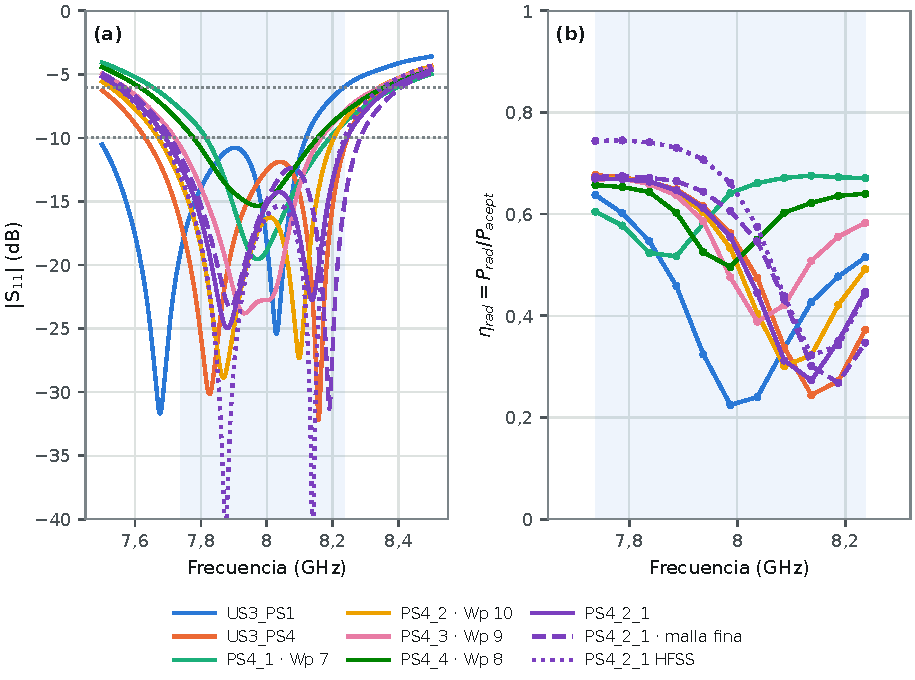
\includegraphics[width=0.95\textwidth]{../figures/res_linea_PS4.pdf}
    \caption{Rama PS4 de la familia con parásito enterrado: $|S_{11}|$ (arriba) y $\eta_\mathrm{rad}$
    (abajo) de US3\_PS1, US3\_PS4, el barrido de $W_p$ de \SI{11}{mm} a \SI{7}{mm} y US3\_PS4\_2\_1.
    La banda del canal 9 aparece sombreada. Fuente: simulaciones de openEMS en malla base; la malla fina y HFSS, donde existen.}
    \label{fig:lineas_ps4}
\end{figure}

\begin{figure}[H]
    \centering
    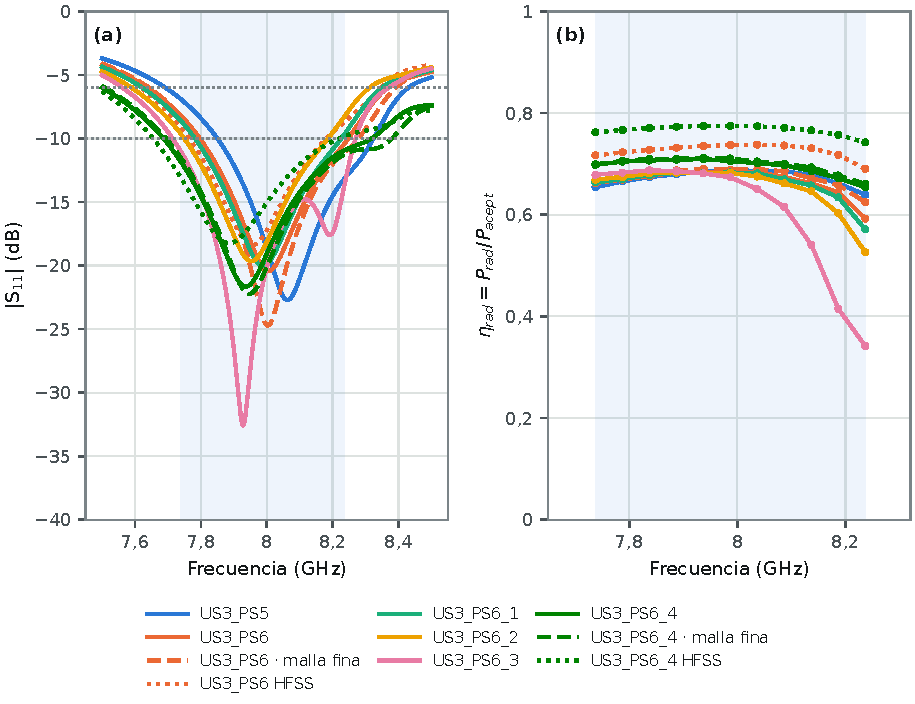
\includegraphics[width=0.95\textwidth]{../figures/res_linea_PS6.pdf}
    \caption{Rama PS6: $|S_{11}|$ (arriba) y $\eta_\mathrm{rad}$ (abajo) de US3\_PS5, US3\_PS6,
    US3\_PS6\_1, US3\_PS6\_2, US3\_PS6\_3 y US3\_PS6\_4. La banda del canal 9 aparece sombreada.
    Fuente: simulaciones de openEMS en malla base; la malla fina y HFSS, donde existen.}
    \label{fig:lineas_ps6}
\end{figure}

\subsection{Resultados del elemento}\label{sec:resultados_elemento}
La Figura~\ref{fig:geom_candidatos} muestra la geometría de los candidatos. Las imágenes son
representaciones 3D generadas a partir de la descripción geométrica de cada diseño, no capturas de
HFSS. La Figura~\ref{fig:geom_cotas} acota la planta de US3\_PS6\_4, y la Figura~\ref{fig:apilado}
muestra el corte del apilado, con el parásito enterrado a media altura del sustrato.

\begin{figure}[H]
    \centering
    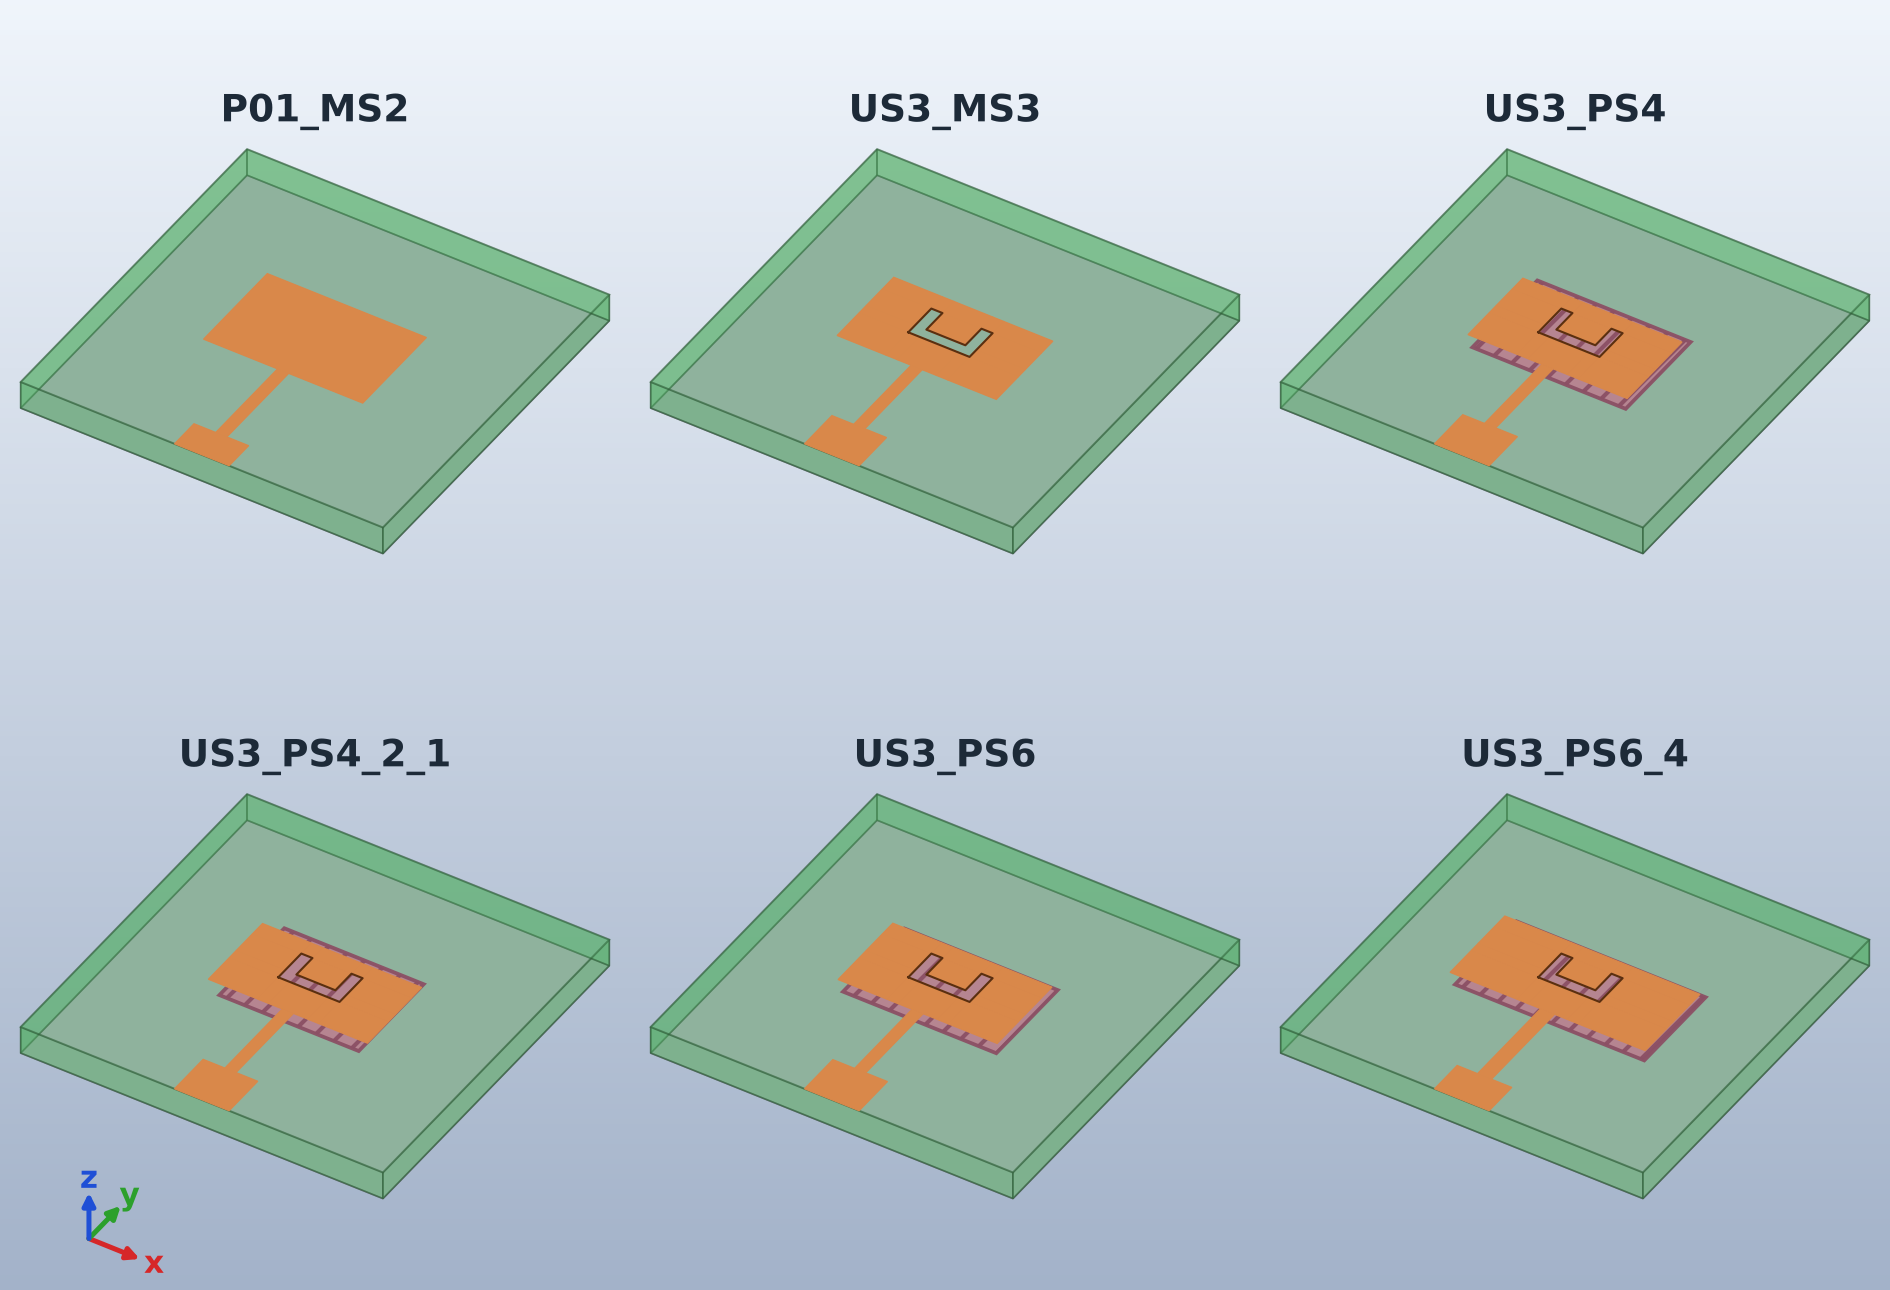
\includegraphics[width=\textwidth]{../figures/geom_candidatos.png}
    \caption{Modelo 3D de los candidatos P01\_MS2, US3\_MS3, US3\_PS4, US3\_PS4\_2\_1, US3\_PS6 y
    US3\_PS6\_4. Representación generada a partir de la geometría del diseño (no es una captura de
    HFSS); el parásito enterrado aparece visible.}
    \label{fig:geom_candidatos}
\end{figure}

\begin{figure}[H]
    \centering
    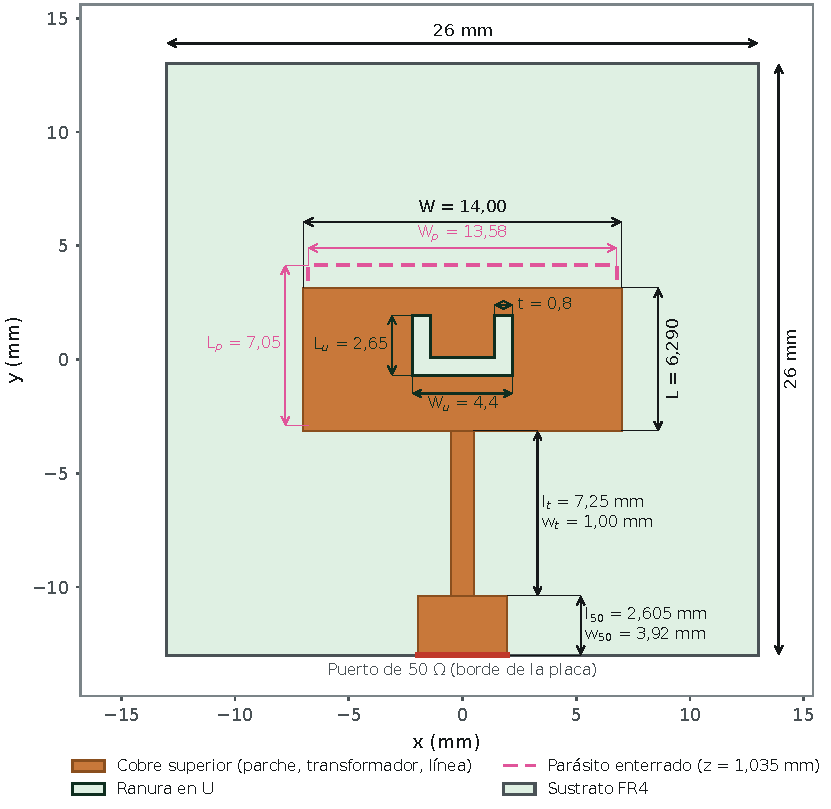
\includegraphics[width=0.8\textwidth]{../figures/geom_US3_PS6_4_cotas.pdf}
    \caption{Vista en planta de US3\_PS6\_4 con las cotas principales: anchura y longitud del parche,
    ranura en U, parásito (en línea discontinua), transformador, línea de \SI{50}{\ohm} y placa de
    \SI{26}{mm} $\times$ \SI{26}{mm}. Fuente: descripción geométrica del diseño.}
    \label{fig:geom_cotas}
\end{figure}

\begin{figure}[H]
    \centering
    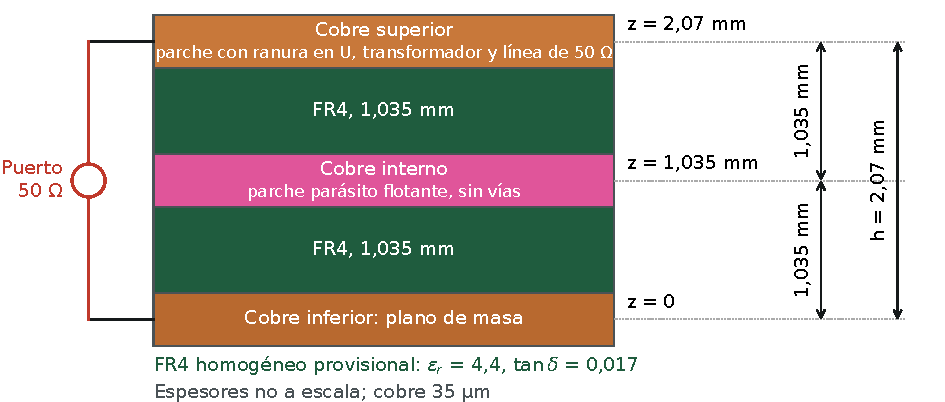
\includegraphics[width=0.8\textwidth]{../figures/geom_apilado.pdf}
    \caption{Esquema del apilado de capas de US3\_PS6\_4 (no a escala; el cobre, de \SI{35}{\micro m}, se dibuja ampliado). Sobre el plano de masa se disponen dos capas de FR-4 de \SI{1.035}{mm} ($h = \SI{2.07}{mm}$; $\varepsilon_r = 4{,}4$, $\tan\delta = 0{,}017$, modelo homogéneo provisional), con el parche parásito flotante, sin vías, en el cobre interno ($z = \SI{1.035}{mm}$). El cobre superior aloja el parche con ranura en U, el transformador y la línea de \SI{50}{\ohm}, donde se sitúa el puerto.}
    \label{fig:apilado}
\end{figure}

La Figura~\ref{fig:s11_candidatos} compara $|S_{11}|$ de los candidatos en el canal. La
Figura~\ref{fig:smith} muestra el lazo de impedancia en la carta de Smith, con el canal en trazo
grueso. Las figuras~\ref{fig:eta} y~\ref{fig:ganancia} recogen la eficiencia y la ganancia realizada
en broadside, y la Figura~\ref{fig:tau} el rizado diagnóstico del retardo de grupo radiado.

\begin{figure}[H]
    \centering
    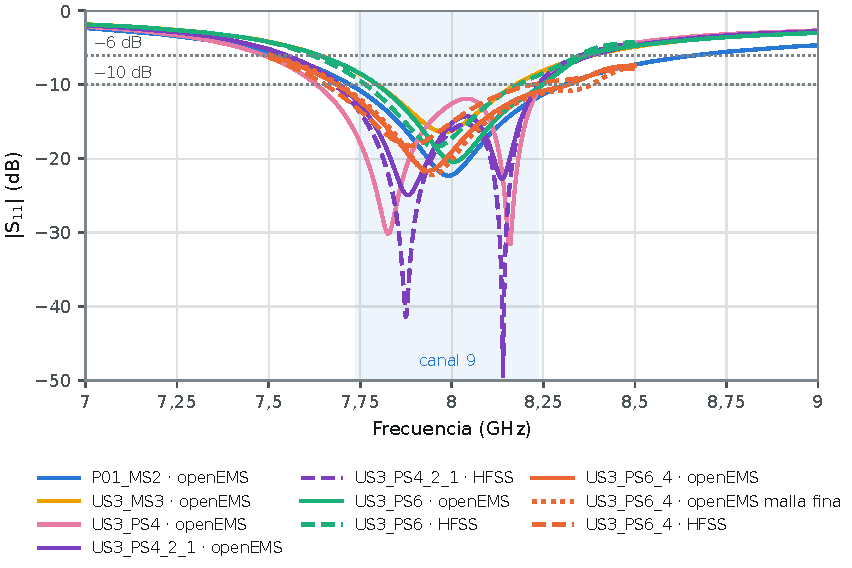
\includegraphics[width=0.85\textwidth]{../figures/res_s11_candidatos.pdf}
    \caption{$|S_{11}|$ de los candidatos en la banda del canal 9. Línea continua: openEMS con malla
    base; línea discontinua: HFSS donde existe (US3\_PS4\_2\_1, US3\_PS6 y US3\_PS6\_4). La malla fina de US3\_PS6\_4 aparece en línea de puntos. La banda del canal aparece sombreada. Fuente:
    simulaciones de openEMS y de HFSS.}
    \label{fig:s11_candidatos}
\end{figure}

\begin{figure}[H]
    \centering
    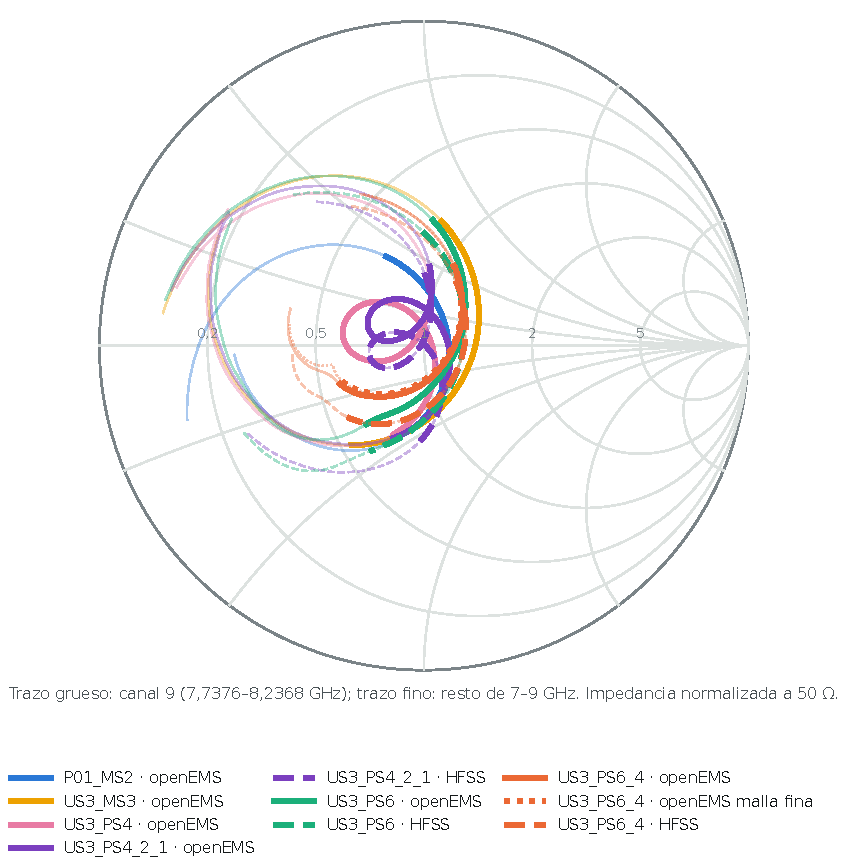
\includegraphics[width=0.7\textwidth]{../figures/res_smith_candidatos.pdf}
    \caption{Carta de Smith de los candidatos, con el canal del trazo grueso. Fuente: simulaciones de
    openEMS y de HFSS.}
    \label{fig:smith}
\end{figure}

\begin{figure}[H]
    \centering
    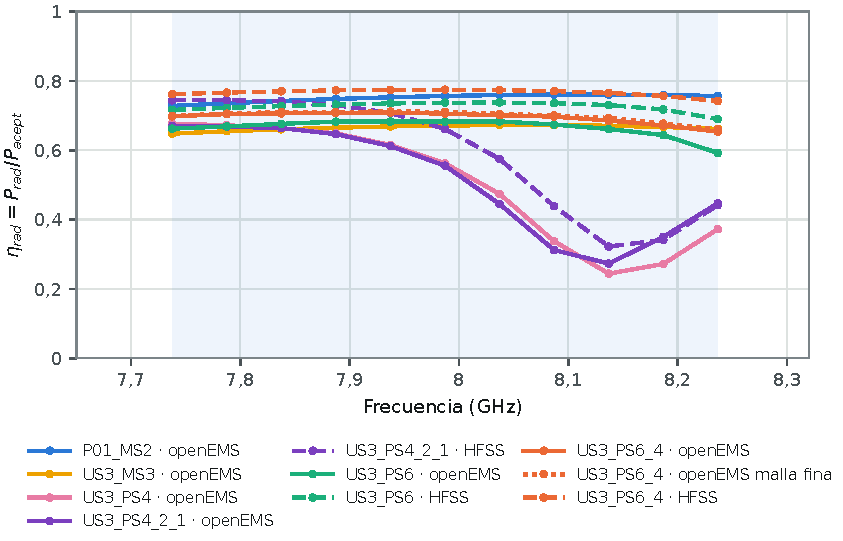
\includegraphics[width=0.68\textwidth]{../figures/res_eta_candidatos.pdf}
    \caption{Eficiencia de radiación $\eta_\mathrm{rad}$ en el canal de los candidatos. Fuente:
    openEMS (malla base) y HFSS donde existe.}
    \label{fig:eta}
\end{figure}

\begin{figure}[H]
    \centering
    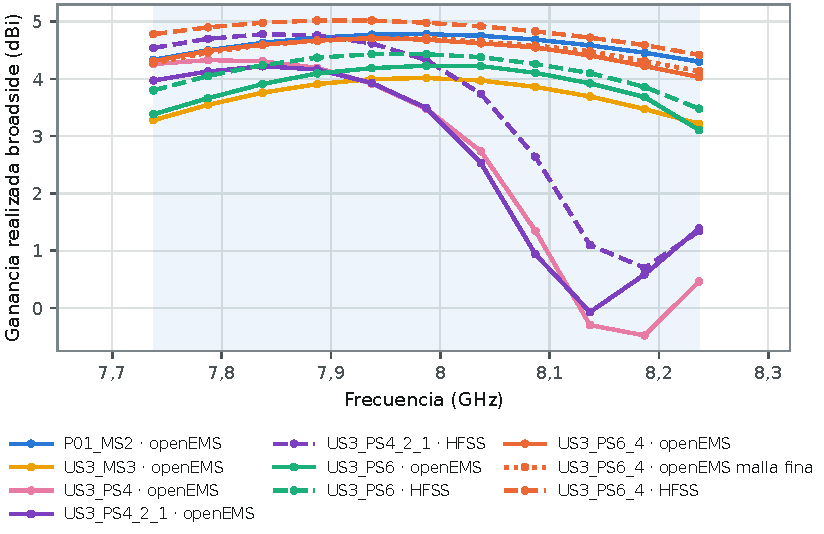
\includegraphics[width=0.68\textwidth]{../figures/res_ganancia_candidatos.pdf}
    \caption{Ganancia realizada en broadside de los candidatos. La malla fina de US3\_PS6\_4 aparece en línea de puntos. Fuente: openEMS (malla base) y HFSS
    donde existe.}
    \label{fig:ganancia}
\end{figure}

\begin{figure}[H]
    \centering
    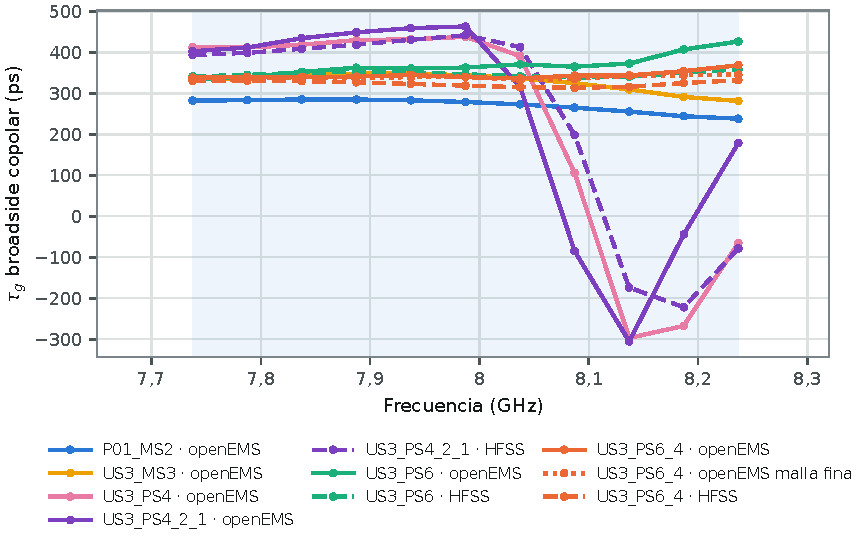
\includegraphics[width=0.85\textwidth]{../figures/res_tau_candidatos.pdf}
    \caption{Retardo de grupo radiado en broadside, copolar, como diagnóstico del rizado. Fuente:
    fase del campo lejano de openEMS (malla base) y de HFSS. La malla fina de US3\_PS6\_4 aparece en línea de puntos. Con once puntos de frecuencia, los
    picos son indicativos.}
    \label{fig:tau}
\end{figure}

La Tabla~\ref{tab:candidatos} compara los cuatro candidatos. Para US3\_PS4\_2\_1 y US3\_PS6 se
incluyen también los datos de HFSS. Los valores de openEMS son de la malla base y de la fina. El
rizado del retardo de grupo de openEMS no se ha calculado para todas las mallas, y no es directamente
comparable con el de HFSS, porque se obtiene con una formulación de diagnóstico distinta.

\begin{table}[H]
    \centering
    \caption{Candidatos del elemento. Adaptación ($|S_{11}|$): \texttt{EM\_SIMULATED} en openEMS y en HFSS, con puerto concentrado. Radiación ($\eta_\mathrm{rad}$, ganancia y rizado): HFSS con elemento aislado y convergencia adaptativa, \texttt{HFSS\_VALIDATED} con la reserva del puerto. La ganancia es la realizada en broadside. En HFSS, la ganancia de US3\_PS4\_2\_1 y de US3\_PS6 se da en cuatro frecuencias (7,7376; 7,9872; 8,1370 y 8,2368 GHz) y la eficiencia, en las once frecuencias analizadas; la de P01\_MS2, en tres frecuencias (7,7376; 7,9872 y 8,2368 GHz). Los intervalos de US3\_PS6\_4 se refieren al canal; los de P01\_MS2, a las tres frecuencias indicadas.}
    \label{tab:candidatos}
    {\small
    \begin{tabularx}{\textwidth}{l l *{5}{>{\centering\arraybackslash}X}}
        \toprule
        Diseño & Fuente & Peor $|S_{11}|$ (\si{dB}) & Canal $\le -10$\,\si{dB} & $\eta_\mathrm{rad}$ & $G_\mathrm{real}$ (\si{dBi}) & Rizado $\tau_g$ (\si{ps}, pico a pico) \\
        \midrule
        P01\_MS2 & openEMS, base & $-10{,}42$ & sí & $0{,}73$--$0{,}76$ & $4{,}3$--$4{,}8$ & $\approx 47$ \\
        P01\_MS2 & openEMS, fina & $-10{,}36$ & sí & $0{,}73$--$0{,}76$ & $4{,}3$--$4{,}8$ & $\approx 48$ \\
        P01\_MS2 & HFSS & $-9{,}81$ & no (\SI{98.2}{\percent}) & $0{,}81$--$0{,}85$ & $4{,}7$--$5{,}2$ & no comparable \\
        \midrule
        US3\_PS4\_2\_1 & openEMS, base & $-10{,}35$ & sí & $0{,}27$--$0{,}67$ & $-0{,}1$--$4{,}2$ & no comparable \\
        US3\_PS4\_2\_1 & openEMS, fina & $-11{,}38$ & sí & $0{,}27$--$0{,}68$ & $-0{,}1$--$4{,}3$ & no comparable \\
        US3\_PS4\_2\_1 & HFSS & $-10{,}00$ (justo) & sí (límite) & $0{,}32$--$0{,}74$ & $1{,}1$--$4{,}5$ & $\approx 664$ \\
        \midrule
        US3\_PS6 & openEMS, base & $-8{,}16$ & no (\SI{88}{\percent}) & $0{,}59$--$0{,}68$ & $3{,}1$--$4{,}2$ & no comparable \\
        US3\_PS6 & openEMS, fina & $-8{,}14$ & no (\SI{88}{\percent}) & $0{,}63$--$0{,}69$ & $3{,}4$--$4{,}3$ & no comparable \\
        US3\_PS6 & HFSS & $-8{,}72$ & no (\SI{83.6}{\percent}) & $0{,}69$--$0{,}74$ & $3{,}5$--$4{,}4$ & $\approx 20$ \\
        \midrule
        US3\_PS6\_4 & openEMS, base & $-10{,}92$ & sí & $0{,}65$--$0{,}71$ & $4{,}0$--$4{,}7$ & $\approx 32$ \\
        US3\_PS6\_4 & openEMS, fina & $-11{,}24$ & sí & $0{,}66$--$0{,}71$ & $4{,}1$--$4{,}7$ & $\approx 15$ \\
        US3\_PS6\_4 & HFSS & $-9{,}82$ & no (\SI{96.4}{\percent}) & $0{,}74$--$0{,}78$ & $4{,}4$--$5{,}0$ & $\approx 18$ \\
        \bottomrule
    \end{tabularx}
    }
\end{table}

La lectura de la tabla es clara. P01\_MS2 es el más eficiente, cumple \SI{-10}{dB} en openEMS y tiene poco rizado
del retardo de grupo (unos \SI{47}{ps} en openEMS), pero su margen de adaptación es estrecho y en HFSS queda a \SI{0.19}{dB} de \SI{-10}{dB}. US3\_PS4\_2\_1 cubre el canal, pero en la mitad
alta su eficiencia cae hasta $0{,}32$ en HFSS y su retardo de grupo radiado rizado llega a unos
\SI{664}{ps}. US3\_PS6 radia de forma uniforme y con poco rizado, pero no llega a \SI{-10}{dB}.
US3\_PS6\_4 combina las dos cosas en openEMS: cubre el canal con eficiencia plana y rizado pequeño. En HFSS mantiene la eficiencia y el rizado, pero su peor punto queda en \SI{-9.82}{dB}, en el borde superior del canal (Sección~\ref{sec:ps6_4_hfss}).

\paragraph{P01\_MS2 en HFSS.} El elemento P01\_MS2 se simuló en HFSS con la geometría de su diseño, un puerto concentrado de \SI{50}{\ohm} en el borde de la placa y un análisis adaptativo con criterio $\Delta S \le 0{,}02$ en una pasada consecutiva. Es un criterio menos estricto que el de $0{,}01$ en dos pasadas que se ha usado con los demás candidatos. La solución convergió en 10 pasadas, con $\Delta S$ final de $0{,}0156$ y 15\,964 tetraedros. Su peor $|S_{11}|$ en el canal es de \SI{-9.81}{dB}, en el borde superior (\SI{8.236}{GHz}), y el mínimo, de \SI{-22.0}{dB}, está en \SI{7.937}{GHz}. Todo el canal queda por debajo de \SI{-6}{dB}, y el \SI{98.2}{\percent} del canal, por debajo de \SI{-10}{dB}.

El peor caso queda a \SI{0.19}{dB} del objetivo de \SI{-10}{dB}. Con $|S_{11}| \approx 0{,}31$, un $\Delta S$ de $0{,}02$ equivale a unos $\pm 0{,}5$\,dB, así que la adaptación no permite afirmar ni negar el cumplimiento de \SI{-10}{dB} en toda la banda. HFSS sitúa la resonancia unos \SI{54}{MHz} por debajo de la de openEMS. La eficiencia de radiación queda entre $0{,}81$ y $0{,}85$ en las tres frecuencias de análisis, y la ganancia realizada en broadside, entre \SI{4.7}{dBi} y \SI{5.2}{dBi}. Frente a openEMS, la eficiencia sale entre $0{,}08$ y $0{,}10$ mayor en HFSS, y la ganancia, entre \SI{0.4}{dB} y \SI{0.6}{dB} mayor, con una directividad similar (de \SI{6.0}{dBi} a \SI{6.4}{dBi} en HFSS, frente a \SI{5.8}{dBi}--\SI{6.1}{dBi} en openEMS). La causa no está identificada, y no se promedian ambos resultados. El retardo de grupo radiado solo se ha obtenido en tres frecuencias: con tres puntos se obtiene una variación de unos \SI{-43}{ps} a lo largo del canal, que no es un rizado. Para medir el rizado haría falta el campo lejano en las once frecuencias, que no se ha exportado, por lo que la columna de rizado de este diseño no es comparable con las demás. La adaptación se clasifica como \texttt{EM\_SIMULATED}, y la radiación (eficiencia y ganancia), como \texttt{HFSS\_VALIDATED} con la reserva del puerto concentrado y del criterio de convergencia de $0{,}02$.

\subsection{Comparación entre openEMS y HFSS y sensibilidad de malla}\label{sec:mallas}
La Figura~\ref{fig:hfss_openems} compara $|S_{11}|$ de openEMS y HFSS para US3\_PS4\_2\_1, US3\_PS6 y US3\_PS6\_4.
En la malla base, US3\_PS4\_2\_1 coincide con HFSS: los mínimos quedan a \SI{5}{MHz}
de diferencia, y el peor caso de HFSS (\SI{-10.00}{dB}) es casi el de openEMS (\SI{-10.35}{dB}). La
malla fina de openEMS, en cambio, desplaza la resonancia superior unos \SI{53}{MHz}, y HFSS no
reproduce ese desplazamiento. Para US3\_PS6, HFSS sitúa el mínimo unos \SI{50}{MHz} por debajo del de
openEMS (\SI{7.955}{GHz} frente a \SI{8.005}{GHz}) y el peor caso pasa al borde superior, con
\SI{-8.72}{dB}. El desfase observado es menor que los \SIrange{60}{75}{MHz} que se habían supuesto a
partir de diseños sin parásito, y no tiene una causa identificada.

\begin{figure}[H]
    \centering
    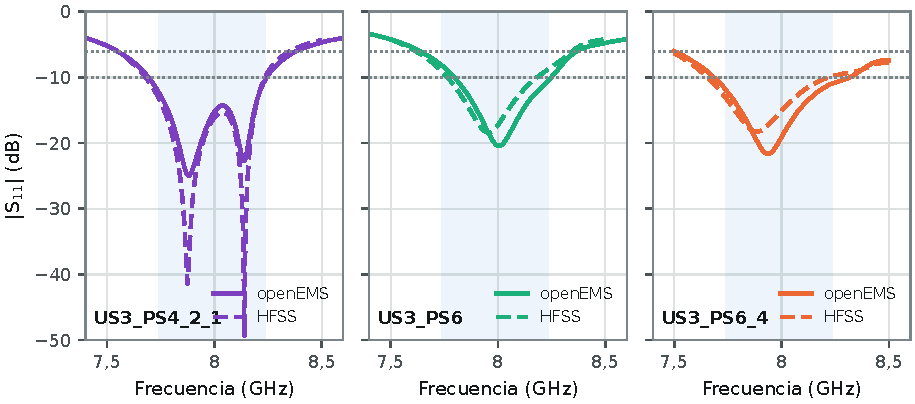
\includegraphics[width=0.85\textwidth]{../figures/res_hfss_openems.pdf}
    \caption{$|S_{11}|$ de US3\_PS4\_2\_1, US3\_PS6 y US3\_PS6\_4 (tres paneles): openEMS (mallas base y fina) frente a HFSS en la
    banda del canal 9. Fuente: simulaciones de openEMS y de HFSS.}
    \label{fig:hfss_openems}
\end{figure}

La sensibilidad de malla es muy distinta de un diseño a otro, y eso condiciona la confianza que se
puede poner en cada resultado. La Tabla~\ref{tab:mallas} resume los pares de mallas.

\begin{table}[H]
    \centering
    \caption{Sensibilidad a la malla en openEMS: peor $|S_{11}|$ en el canal en cada malla y máxima
    diferencia $|\Delta\Gamma|$ en el canal entre ambas.}
    \label{tab:mallas}
    \begin{tabularx}{\textwidth}{l c c c}
        \toprule
        Diseño & Peor $|S_{11}|$ base / fina (\si{dB}) & Mallas comparadas & $\max |\Delta\Gamma|$ \\
        \midrule
        P01\_MS2 & $-10{,}42$ / $-10{,}36$ & base y fina & $0{,}029$ \\
        US3\_PS4\_2\_1 & $-10{,}35$ / $-11{,}38$ & base y fina & $0{,}20$ \\
        US3\_PS6 & $-8{,}16$ / $-8{,}14$ & base y fina & $0{,}056$ \\
        US3\_PS6\_4 & $-10{,}92$ / $-11{,}24$ & base y fina & $0{,}015$ \\
        \bottomrule
    \end{tabularx}
\end{table}

US3\_PS4\_2\_1 tiene un $|\Delta\Gamma|$ de $0{,}20$, unas trece veces el de US3\_PS6\_4. Su
resonancia superior se mueve con la malla y el borde superior de la banda de \SI{-10}{dB} cambia unos
\SI{41}{MHz}. Las dos mallas difieren en varias cosas a la vez (resolución de los bordes metálicos,
paso máximo y líneas de sustrato), así que el origen del cambio no está identificado. Para US3\_PS6\_4,
en cambio (Figura~\ref{fig:mallas_ps6_4}), la respuesta es estable: el mínimo único queda en \SI{7.936}{GHz} con la malla base y en
\SI{7.947}{GHz} con la fina, y el borde superior de la región por debajo de \SI{-10}{dB} sube solo
unos \SI{62}{MHz}. Estas dos mallas no son una prueba de convergencia. El refinamiento es de solo
$1{,}25$ a $1{,}43$ veces, y cambian a la vez el grosor de la capa absorbente y la posición de la
caja de campo lejano. Ni siquiera permiten decir cuál de los dos valores es el más cercano al real.
Lo que sí permiten es acotar la sensibilidad de la respuesta.

\begin{figure}[H]
    \centering
    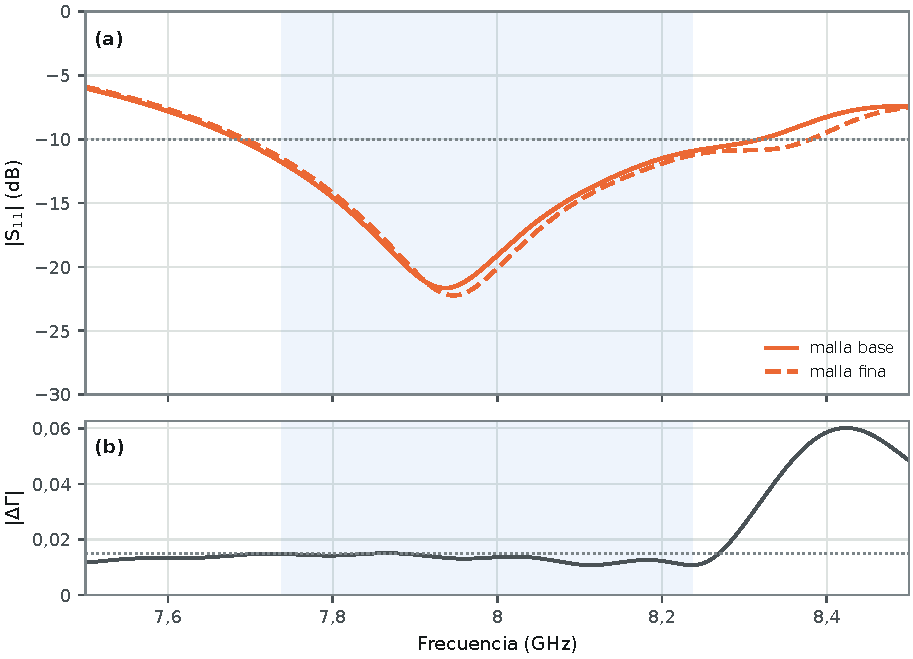
\includegraphics[width=0.85\textwidth]{../figures/res_mallas_PS6_4.pdf}
    \caption{$|S_{11}|$ de US3\_PS6\_4 en la malla base y en la fina, y diferencia $|\Delta\Gamma|$ en el
    canal entre ambas. Fuente: simulaciones de openEMS (malla base y malla fina).}
    \label{fig:mallas_ps6_4}
\end{figure}

\subsection{Elemento US3\_PS6\_4 en HFSS}\label{sec:ps6_4_hfss}
El diseño US3\_PS6\_4 se simuló en HFSS como elemento aislado, con el mismo procedimiento que los anteriores. La convergencia adaptativa se alcanzó en 12 pasadas, con una variación de $S$ en la última pasada de $0{,}0099$, frente al objetivo de $0{,}01$. La última pasada no mejora a la anterior, así que la convergencia es justa.

El peor valor de $|S_{11}|$ en el canal es de \SI{-9.82}{dB}, en \SI{8.236}{GHz}, en el borde superior de la banda. El mínimo es único, en \SI{7.886}{GHz} (\SI{-18.25}{dB}), y la región por debajo de \SI{-10}{dB} va de \SI{7.655}{GHz} a \SI{8.219}{GHz}, un ancho de \SI{563}{MHz}. El \SI{96.4}{\percent} del canal queda por debajo de \SI{-10}{dB}, y el \SI{100}{\percent} por debajo de \SI{-6}{dB}. Las hipótesis de esta simulación se registraron antes de lanzarla: el mínimo debía caer entre \SI{7.86}{GHz} y \SI{7.90}{GHz} (se cumplió); el peor valor, entre \SI{-9.1}{dB} y \SI{-10.9}{dB}, con una probabilidad estimada de cumplir \SI{-10}{dB} de alrededor del \SI{50}{\percent} (el valor cae dentro del rango, pero no cumple \SI{-10}{dB}); y la eficiencia y la ganancia, por encima de $0{,}6$ y de \SI{2}{dBi} (se cumplieron). HFSS desplaza el mínimo unos \SI{-50}{MHz} respecto a openEMS, como ya ocurrió con US3\_PS6, y estrecha la banda por debajo de \SI{-10}{dB}: \SI{563}{MHz} frente a \SI{631}{MHz} y \SI{685}{MHz} en las dos mallas de openEMS. El borde superior de esa región queda en \SI{8.219}{GHz}, por debajo del rango previsto.

La eficiencia de radiación está entre $0{,}742$ y $0{,}775$ en el canal, sin el valle de la familia US3\_PS4. La ganancia realizada en broadside está entre \SI{4.42}{dBi} y \SI{5.02}{dBi}, y su pico, entre \SI{4.50}{dBi} y \SI{5.29}{dBi}, se da inclinado de \SI{5}{\degree} a \SI{15}{\degree} en el plano $yz$. El rizado del retardo de grupo radiado en broadside, copolar, es de \SI{18.4}{ps} sobre los once puntos de frecuencia. Los valores de openEMS y de HFSS se comparan en la Tabla~\ref{tab:candidatos} y en la Figura~\ref{fig:hfss_openems}.

Los \SI{0.18}{dB} que faltan para \SI{-10}{dB} están dentro de la incertidumbre de convergencia. Con $|\Gamma| = 0{,}323$ frente a $0{,}316$ en el umbral, y una variación de $S$ de $0{,}0099$, la incertidumbre equivale a unos $\pm 0{,}27$\,dB alrededor de \SI{-10}{dB}, y el resultado queda entre \SI{-9.55}{dB} y \SI{-10.09}{dB}. No se puede afirmar que el elemento cumpla ni que no cumpla \SI{-10}{dB}. Sí cumple \SI{-6}{dB}, con \SI{3.8}{dB} de margen.

Acortar el parche de \SI{6.29}{mm} a unos \SI{6.22}{mm} subiría el mínimo unos \SI{40}{MHz} a \SI{50}{MHz}, y dejaría el peor valor entre \SI{-10.3}{dB} y \SI{-10.6}{dB} como mucho. Esa mejora es del orden de la tolerancia de grabado y de la incertidumbre de la permitividad del FR-4 provisional, así que \SI{-10}{dB} en toda la banda es un objetivo marginal con este sustrato. Antes de iterar sobre la longitud del parche conviene contrastar la adaptación con un \textit{wave port}: si ese contraste da \SI{-10}{dB} o menos, la variación no hace falta.

\subsection{Array y array virtual}\label{sec:resultados_array}
El array se simuló en HFSS con cinco elementos alineados sobre el eje $x$, con la separación $d$ como
variable de Optimetrics. La Figura~\ref{fig:arr_geom} muestra la geometría del array 1$\times$5 de
US3\_PS6\_4, que es el diseño final, con los puertos numerados del 1 al 5. A \SI{18.2}{mm}, la solución adaptativa alcanzó la convergencia en 16 pasadas, con una variación de $S$ por debajo de $0{,}01$ en las dos últimas (el registro de ese paso declara un objetivo de $0{,}02$, pero el criterio efectivo, como en el resto del barrido, es $0{,}01$). El puerto es concentrado, de \SI{50}{\ohm} en cada elemento, sin modelo de conector y sin contraste con un \textit{wave port}, de modo que las cifras del array se leen con esa reserva.

\begin{figure}[H]
    \centering
    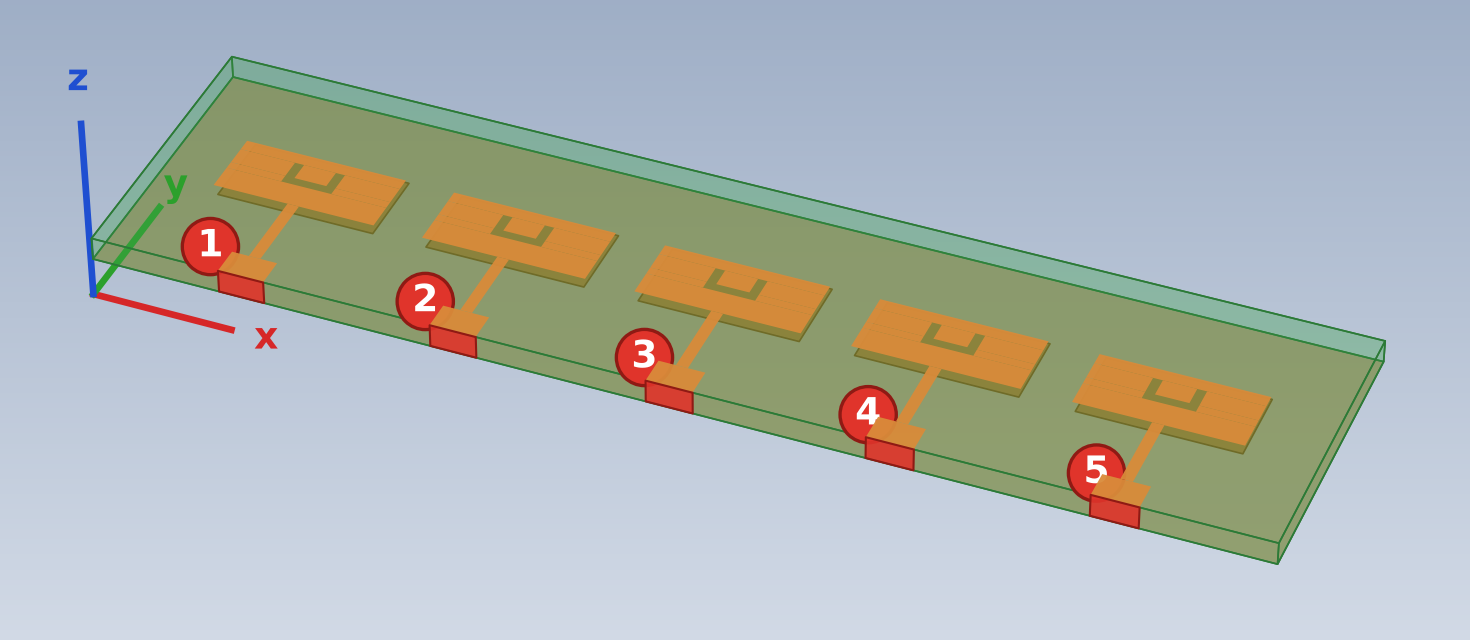
\includegraphics[width=0.7\textwidth]{../figures/arr_geom_1x5_PS6_4.png}
    \caption{Modelo 3D del array 1$\times$5 de US3\_PS6\_4 con paso de \SI{18.2}{mm} y puertos
    numerados del 1 al 5. Representación generada a partir de la geometría del diseño (no es una
    captura de HFSS).}
    \label{fig:arr_geom}
\end{figure}

El paso es el primer parámetro que hay que fijar. Con P01\_MS2 se barrió entre \SI{13.5}{mm} y
\SI{20.5}{mm}, y los resultados muestran un compromiso claro. La Tabla~\ref{tab:paso} recoge algunos
pasos. Con \SI{13.5}{mm}, el paso del artículo de referencia, el acoplo entre vecinos llega a
\SI{-10.3}{dB} y la reflexión activa en broadside es de \SI{-4.9}{dB}, lo que no cumple el criterio
de \SI{-6}{dB}. El acoplo cae de forma monótona al aumentar el paso, y el cruce de \SI{-6}{dB} de la
reflexión activa en broadside está hacia \SI{14.3}{mm}. Por encima de \SI{18}{mm} la reflexión activa
queda por debajo de \SI{-8}{dB} hasta \SI{30}{\degree}. Con US3\_PS6\_4 se repitió el barrido de
paso, como se describe a continuación.

\begin{table}[H]
    \centering
    \caption{Acoplo y adaptación activa del array 1$\times$5 de P01\_MS2 en HFSS para varios pasos,
    peor caso en el canal. La reflexión activa se calcula con los cinco puertos excitados, amplitud
    uniforme y fase progresiva.}
    \label{tab:paso}
    {\small
    \begin{tabularx}{\textwidth}{c *{5}{>{\centering\arraybackslash}X}}
        \toprule
        Paso (\si{mm}) & Adaptación pasiva (\si{dB}) & Acoplo entre vecinos (\si{dB}) & Activa a $0\si{\degree}$ (\si{dB}) & Activa a $15\si{\degree}$ (\si{dB}) & Activa a $30\si{\degree}$ (\si{dB}) \\
        \midrule
        13,5 & $-9{,}6$ & $-10{,}3$ & $-4{,}9$ & $-6{,}3$ & $-6{,}6$ \\
        17,0 & $-10{,}0$ & $-15{,}0$ & $-8{,}5$ & $-9{,}3$ & $-7{,}8$ \\
        18,2 & $-10{,}3$ & $-16{,}9$ & $-9{,}3$ & $-9{,}8$ & $-8{,}1$ \\
        20,5 & $-10{,}7$ & $-20{,}6$ & $-11{,}2$ & $-10{,}4$ & $-8{,}9$ \\
        \bottomrule
    \end{tabularx}
    }
\end{table}

Con US3\_PS6\_4 se simularon once pasos, de \SI{16}{mm} a \SI{20.5}{mm}, en pasos de \SI{0.5}{mm}. El acoplo entre vecinos baja de forma monótona, de \SI{-12.64}{dB} a \SI{16}{mm} a \SI{-20.93}{dB} a \SI{20.5}{mm}, y la reflexión activa a broadside mejora de \SI{-8.34}{dB} a \SI{-11.27}{dB}. La adaptación pasiva no sigue esa tendencia: el peor $S_{ii}$ va de \SI{-11.66}{dB} a \SI{16}{mm} hasta \SI{-10.73}{dB} a \SI{18.2}{mm}, que es el peor de los once pasos, y vuelve a \SI{-11.22}{dB} a \SI{20}{mm}. A \SI{18.2}{mm}, la reflexión activa a broadside no cumple \SI{-10}{dB} (peor puerto de \SI{-9.23}{dB}), y sí lo cumple a partir de \SI{19}{mm} (\SI{-10.13}{dB}). Como $d \le \lambda/2$ en todo el canal para \SI{18.2}{mm}, el valor de \SI{18.2}{mm} se mantiene como compromiso entre acoplo, adaptación activa y ausencia de lóbulos de rejilla, con el coste señalado en la adaptación pasiva y en la activa a broadside.

La Figura~\ref{fig:arr_barrido} resume el HPBW físico y el virtual frente al paso para P01\_MS2 y US3\_PS4\_2\_1. Con P01\_MS2 a \SI{17}{mm} el HPBW físico es de \SI{21.7}{\degree} y el virtual de \SI{17.7}{\degree}, mientras que a \SI{13.5}{mm} son \SI{27.5}{\degree} y \SI{22.9}{\degree}. Los haces de US3\_PS6\_4 solo se han calculado a \SI{18.2}{mm}: a la frecuencia central, el HPBW físico en el plano $xz$ es de \SI{20.5}{\degree} y el virtual, de \SI{16.3}{\degree}. La Figura~\ref{fig:arr_cortes} muestra los cortes normalizados con ambos anchos marcados. Apuntando a \SI{15}{\degree} y a \SI{30}{\degree}, el HPBW físico es de \SI{21.2}{\degree} y \SI{23.2}{\degree}, y el virtual, de \SI{17.2}{\degree} y \SI{18.8}{\degree}. Con US3\_PS4\_2\_1 a la misma separación, los valores son \SI{20.7}{\degree} y \SI{16.4}{\degree}, a \SI{0.2}{\degree} y \SI{0.1}{\degree} de los de US3\_PS6\_4: la apertura, y no el elemento, fija el haz.

\begin{figure}[H]
    \centering
    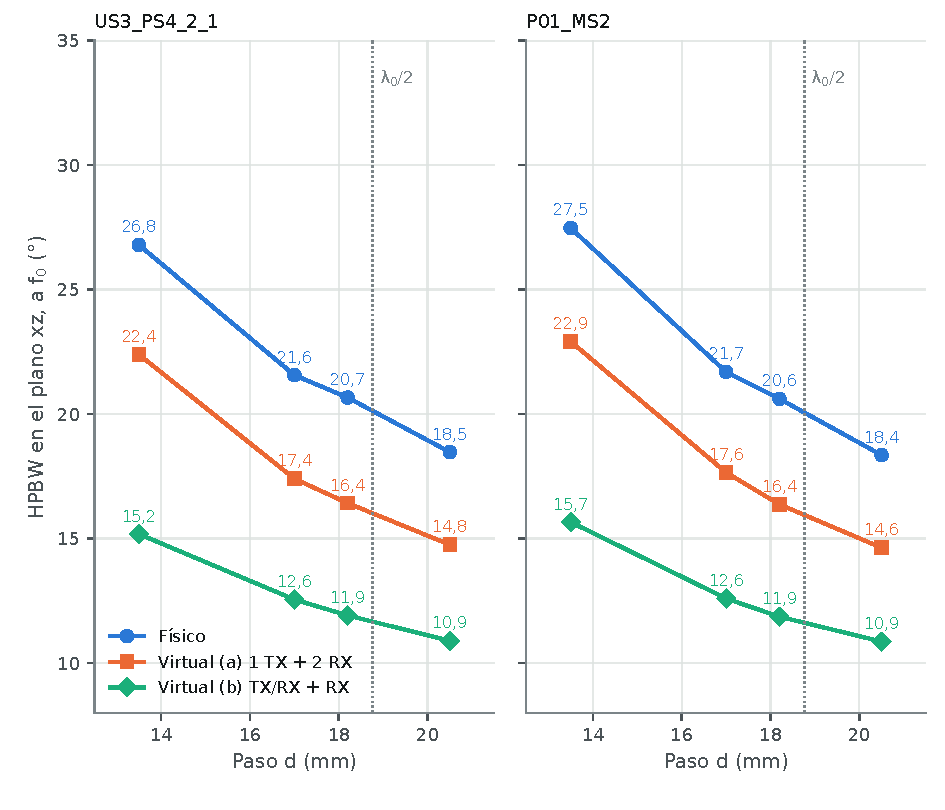
\includegraphics[width=0.85\textwidth]{../figures/arr_barrido_paso.pdf}
    \caption{HPBW físico y virtual en el plano $xz$ frente al paso $d$ para los arrays $1\times 5$ de US3\_PS4\_2\_1 y P01\_MS2 (tres series por elemento: físico, virtual solo biestático y virtual con monostáticos), en los cuatro pasos analizados en detalle. La línea punteada es $\lambda_0/2$ (\SI{18.8}{mm}). Fuente: \texttt{array\_analysis\_d*.json} y \texttt{virtual\_mono/*.json} (HFSS).}
    \label{fig:arr_barrido}
\end{figure}

\begin{figure}[H]
    \centering
    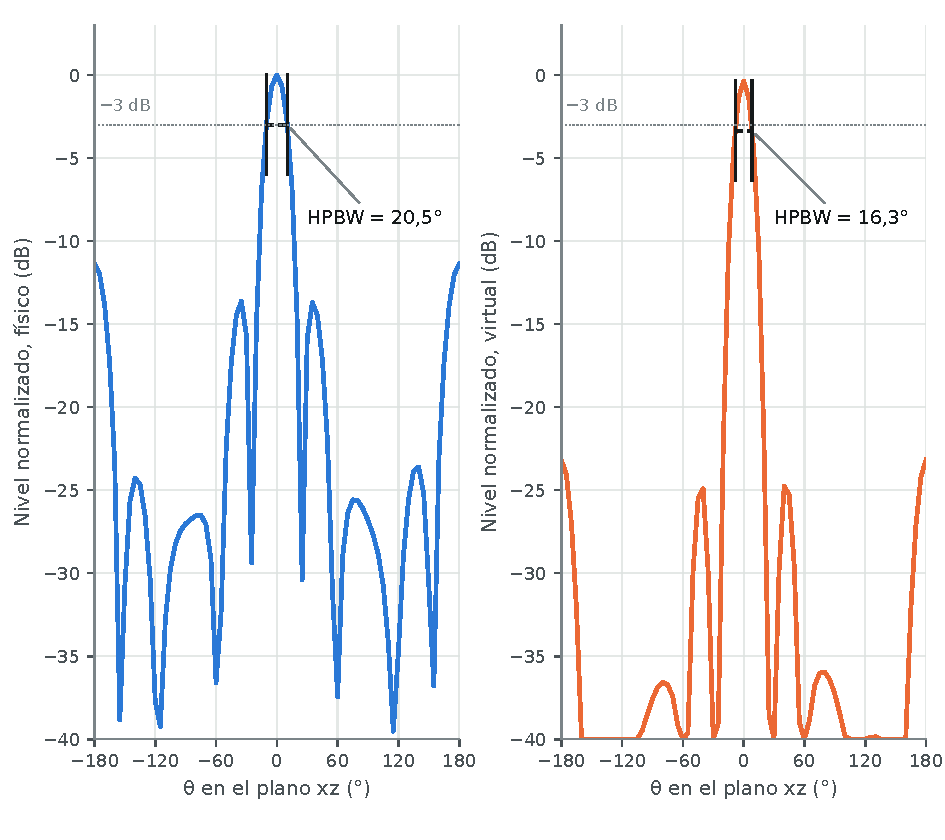
\includegraphics[width=0.85\textwidth]{../figures/arr_cortes_hpbw_PS6_4.pdf}
    \caption{Cortes $xz$ normalizados del array físico y del virtual de US3\_PS6\_4 a la frecuencia
    central, con \SI{18.2}{mm} de paso. Se marcan los HPBW a \SI{-3}{dB}: \SI{20.5}{\degree}
    (físico) y \SI{16.3}{\degree} (virtual, caso a). Fuente: diagramas embebidos exportados de HFSS.}
    \label{fig:arr_cortes}
\end{figure}

La reflexión activa a \SI{15}{\degree} cumple \SI{-10}{dB} en todos los puertos (peor puerto de
\SI{-10.28}{dB}), pero a \SI{30}{\degree} y a \SI{45}{\degree} no (\SI{-8.63}{dB} y \SI{-8.60}{dB}).
En los cuatro ángulos calculados, \SI{0}{\degree}, \SI{15}{\degree}, \SI{30}{\degree} y
\SI{45}{\degree}, cumple \SI{-6}{dB}. La eficiencia radiada sobre la aceptada por puerto está entre
$0{,}73$ y $0{,}77$ en las tres frecuencias calculadas (\SI{7.7376}{GHz}, \SI{7.9872}{GHz} y
\SI{8.2368}{GHz}). El pico del diagrama físico es de \SI{11.48}{dBi} a la frecuencia central y de
\SI{11.10}{dBi} a \SI{8.2368}{GHz}. El retardo de grupo a broadside, sobre las mismas tres
frecuencias, es de \SI{278.6}{ps} a \SI{284.1}{ps} en el trayecto físico de un sentido, con un
rizado de \SI{5.6}{ps}, y de \SI{556.9}{ps} a \SI{569.0}{ps} en el virtual de dos sentidos, con un
rizado de \SI{12.1}{ps}. Con tres frecuencias, estos rizados no son comparables con el del elemento
aislado, que se calculó sobre once puntos.

Las Figuras~\ref{fig:arr_3d_fis} y~\ref{fig:arr_3d_vir} muestran el diagrama tridimensional del
array físico y del virtual a la frecuencia central. En el virtual, la silueta de las posiciones
virtuales aparece sobre la base del diagrama.

\begin{figure}[H]
    \centering
    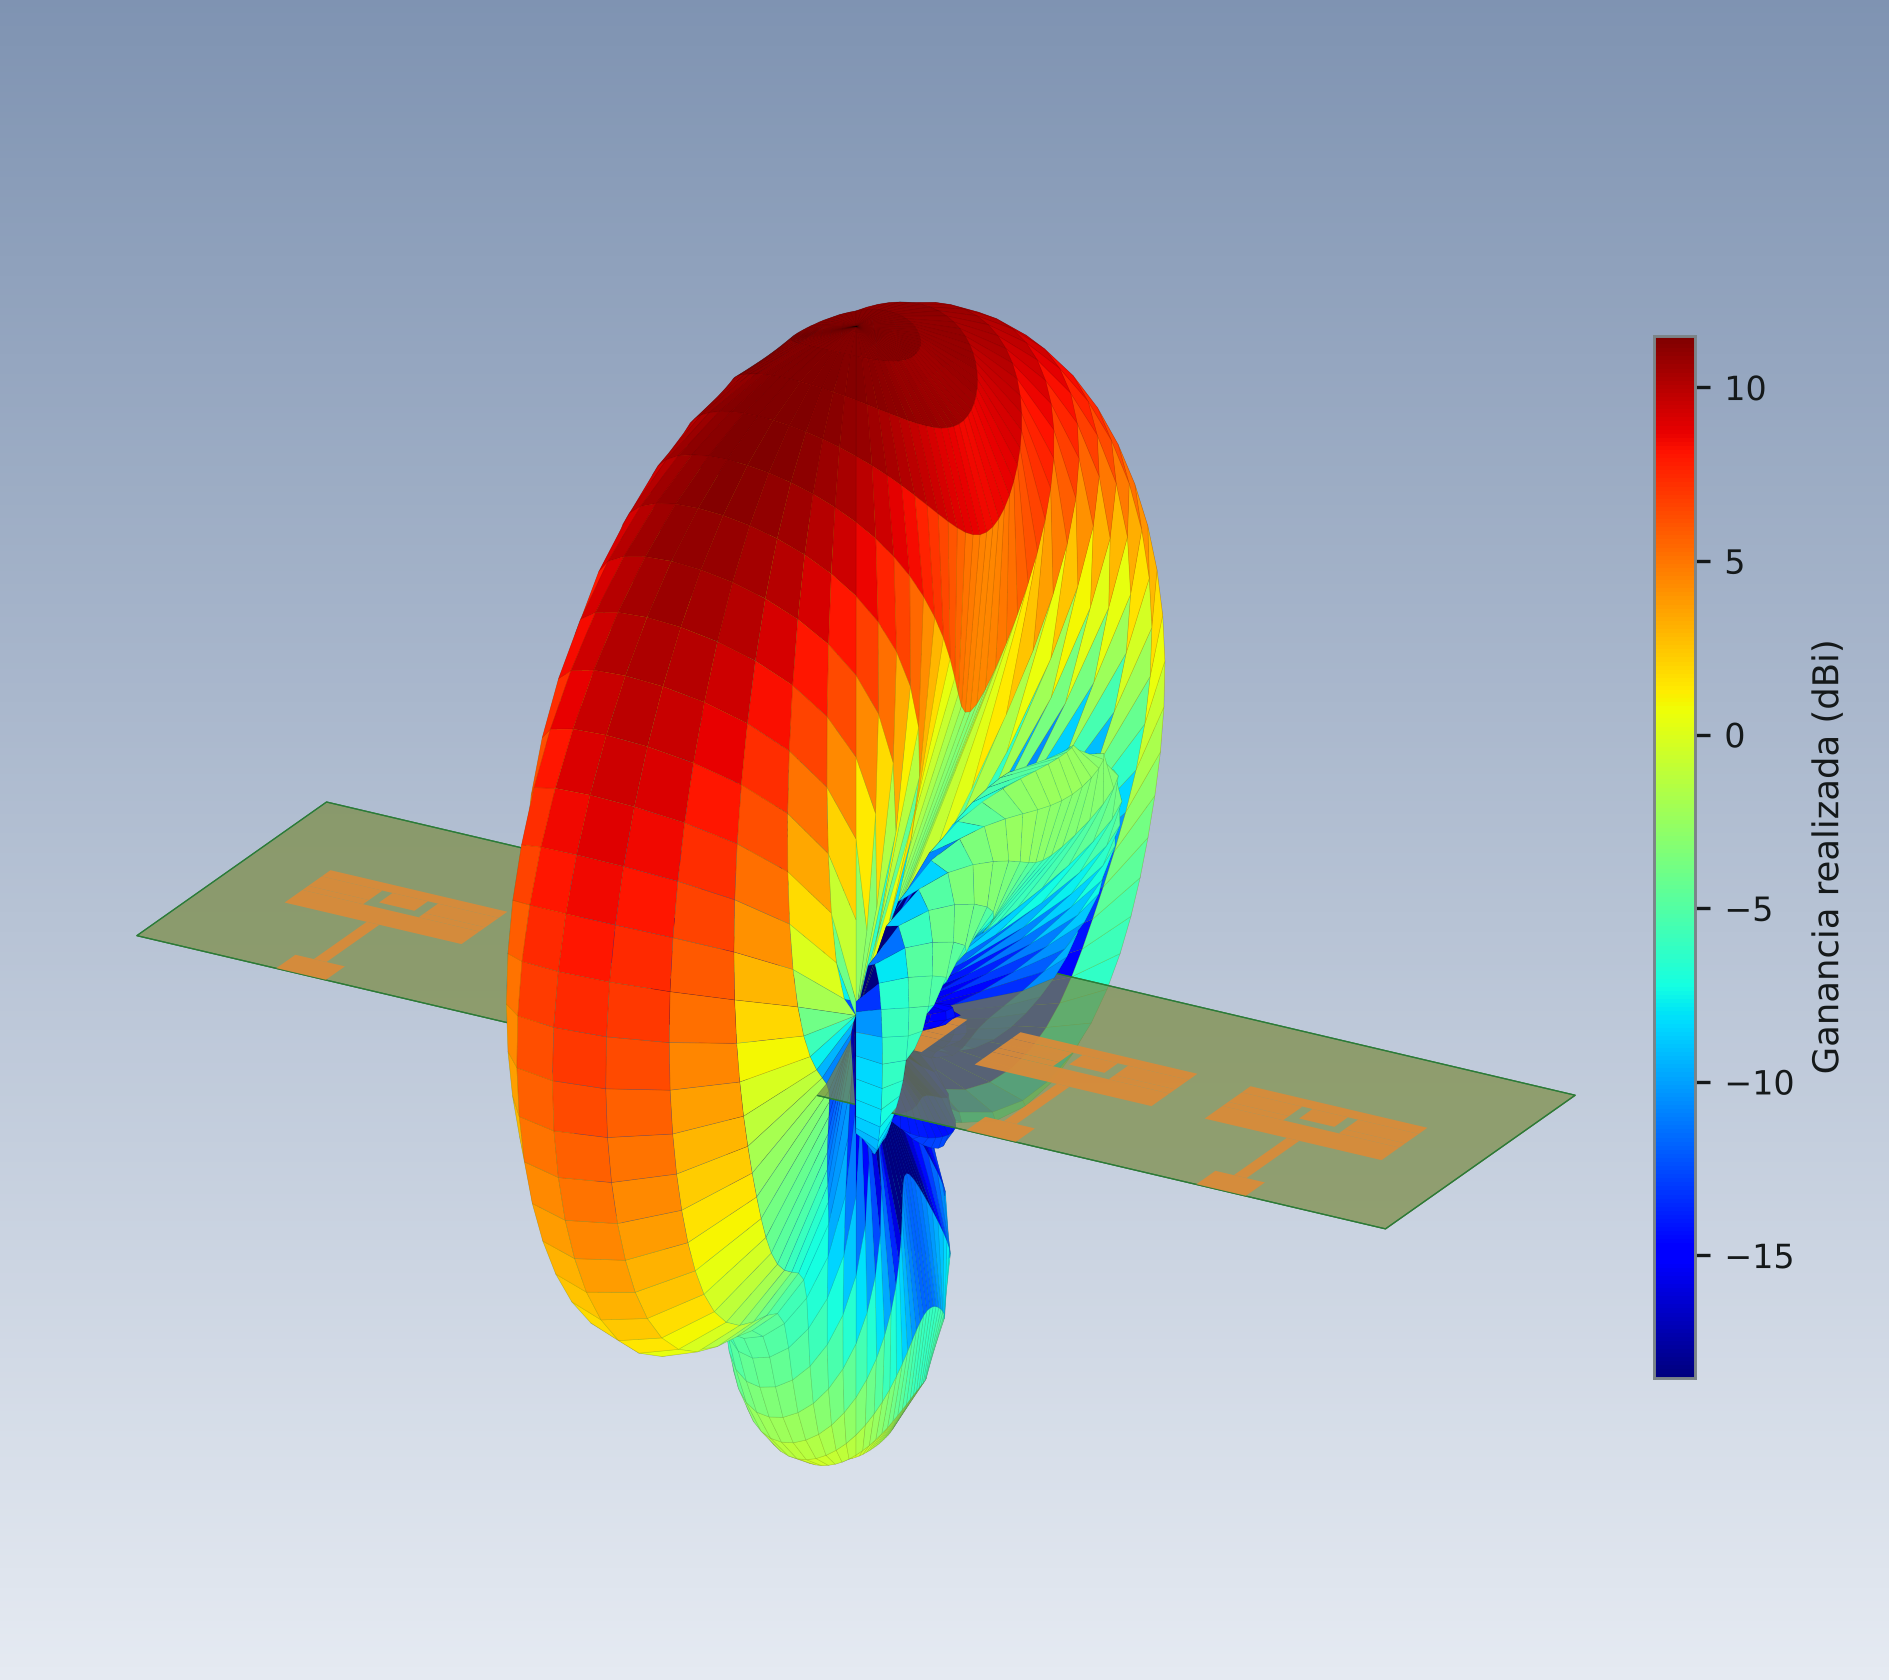
\includegraphics[width=0.8\textwidth]{../figures/arr_patron3d_fisico_PS6_4.png}
    \caption{Diagrama 3D del array físico de US3\_PS6\_4 a la frecuencia central, sobre el plano
    del array. Fuente: diagramas embebidos exportados de HFSS (paso \SI{18.2}{mm}).}
    \label{fig:arr_3d_fis}
\end{figure}

\begin{figure}[H]
    \centering
    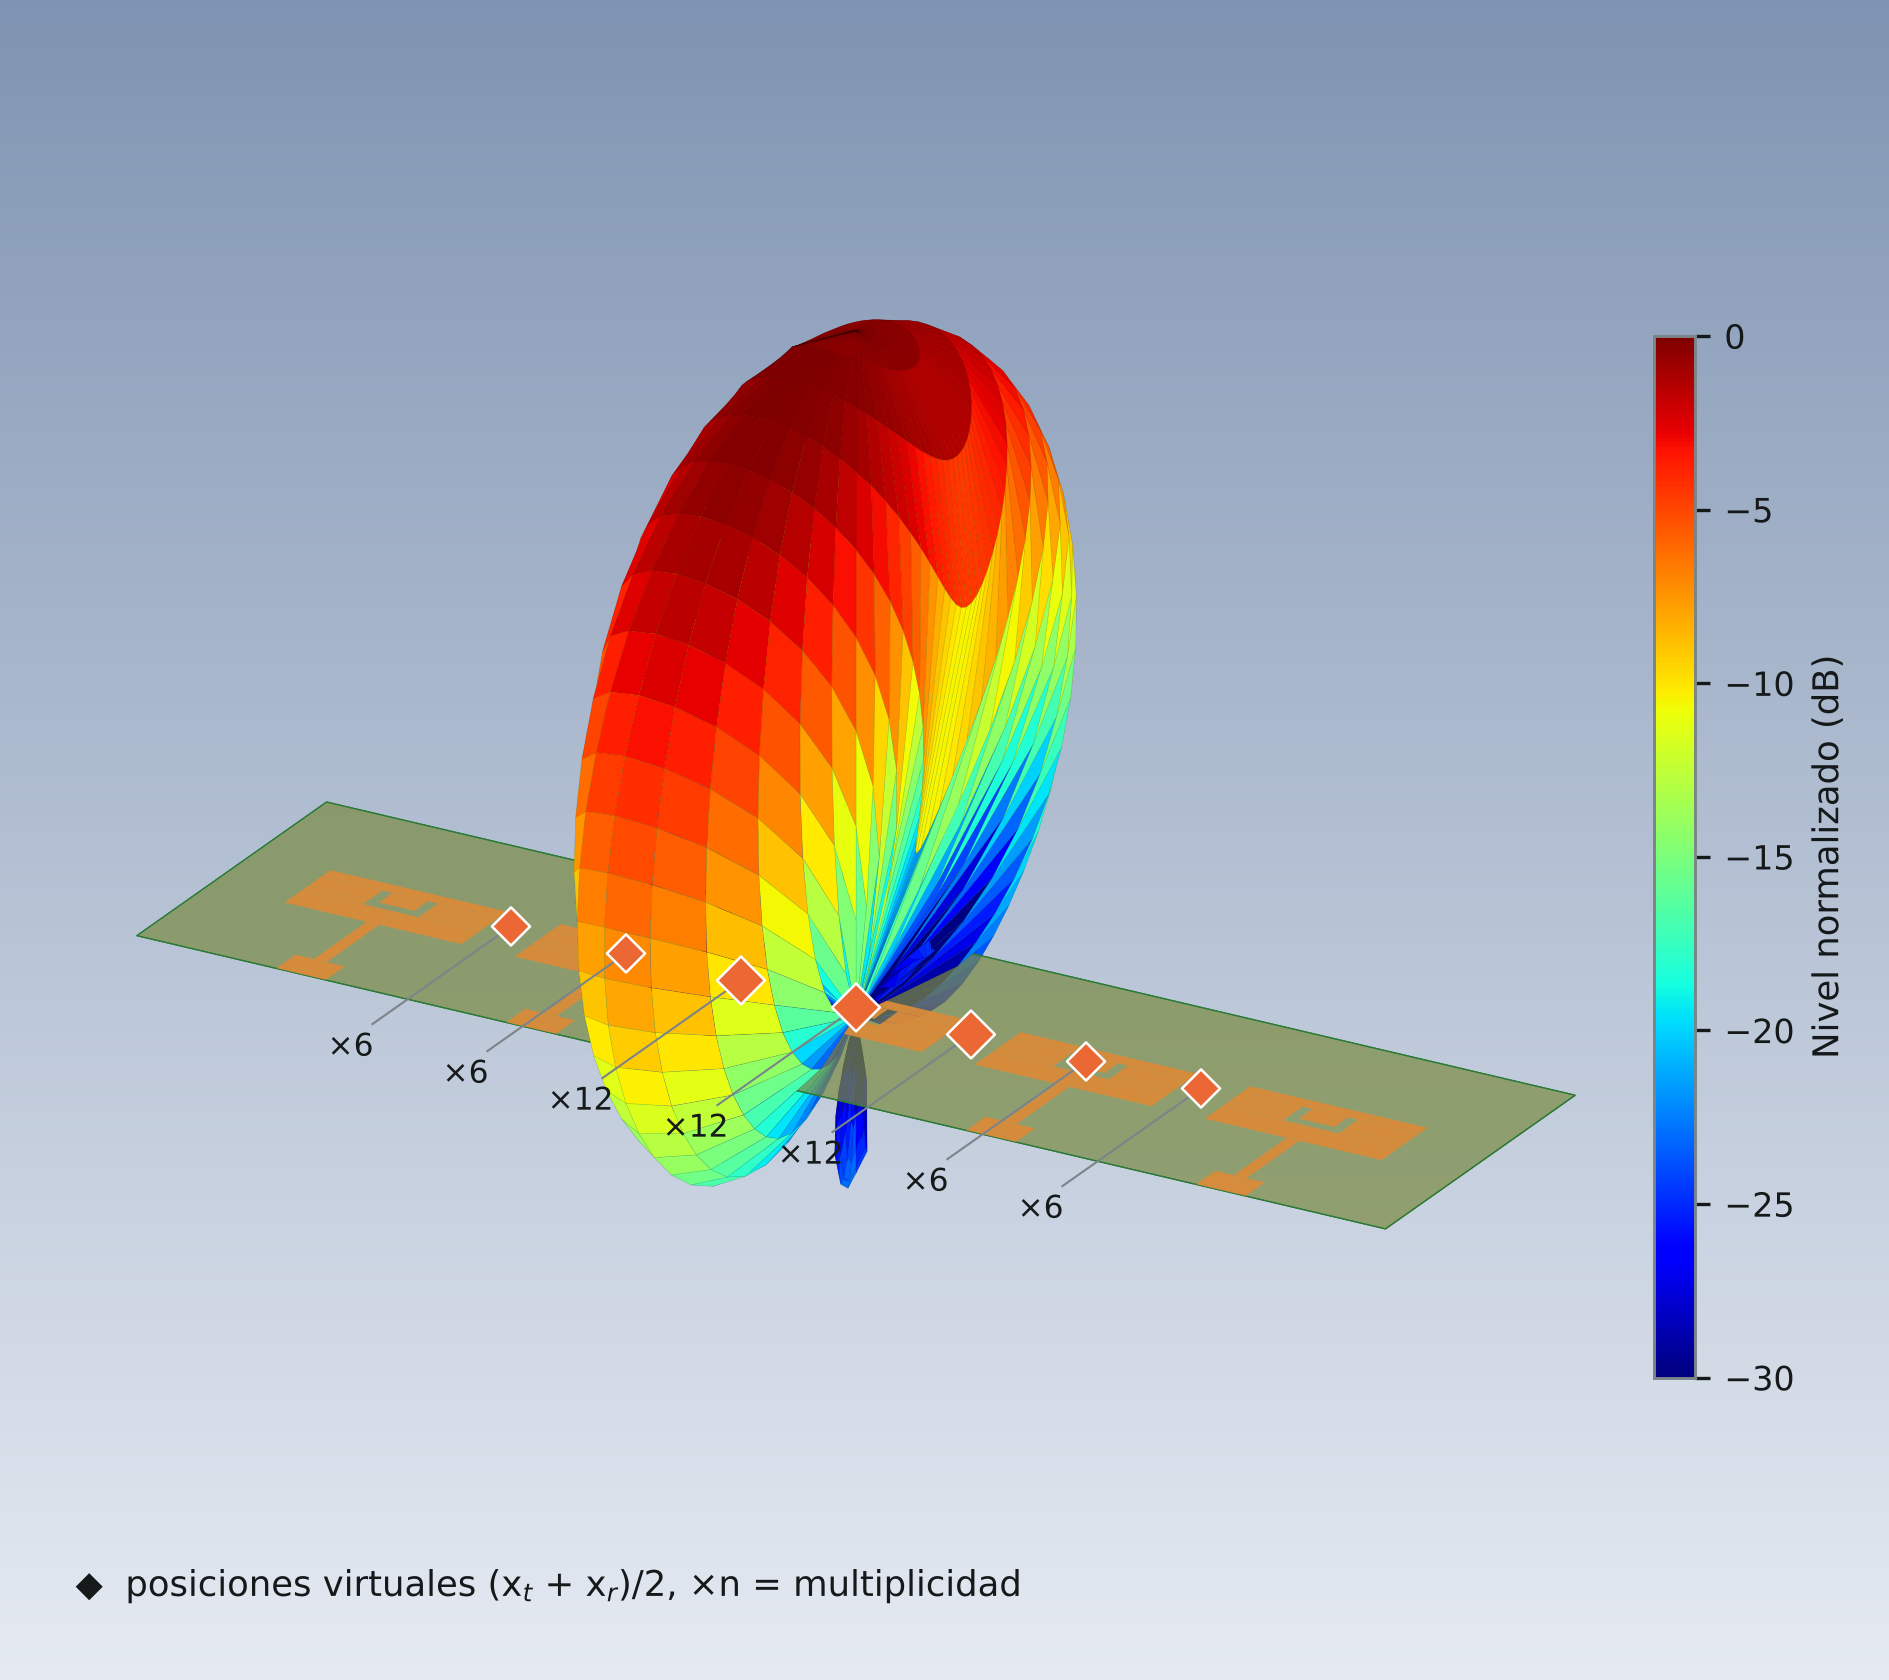
\includegraphics[width=0.8\textwidth]{../figures/arr_patron3d_virtual_PS6_4.png}
    \caption{Diagrama 3D del array virtual de US3\_PS6\_4 a la frecuencia central, con las posiciones
    virtuales $(x_t + x_r)/2$ y su multiplicidad en la base. Fuente: suma coherente de los diagramas embebidos de
    HFSS (paso \SI{18.2}{mm}).}
    \label{fig:arr_3d_vir}
\end{figure}

Las comparaciones anteriores se hacen sobre el array virtual con la convención de la
ecuación~\eqref{eq:suma_coherente}. El array virtual de referencia del artículo tiene un HPBW de
\SI{24.0}{\degree}, con el elemento de aquel trabajo. Los valores de este TFE no son directamente
comparables con esa cifra, porque el elemento, la separación y la apertura son distintos, pero dan
la dirección del resultado: el array virtual del caso (a) estrecha el haz frente al físico y frente
a la referencia.

\paragraph{Array de US3\_PS6.} Con el elemento US3\_PS6 se simuló un array 1$\times$5 con 16 pasos entre \SI{13.5}{mm} y \SI{20.5}{mm}, cada \SI{0.5}{mm} y además \SI{18.2}{mm}. Para cada paso se exportan la matriz $S$ y los diagramas embebidos.

A \SI{18.2}{mm} y a la frecuencia central, la adaptación del peor puerto es de \SI{-8.64}{dB}, cercana a la del elemento aislado, y el acoplo entre vecinos es de \SI{-18.25}{dB} en el peor caso del canal. La reflexión activa en broadside es de \SI{-9.62}{dB}. Los haces en el plano $xz$ tienen un HPBW físico de \SI{20.6}{\degree}, un HPBW virtual de \SI{16.4}{\degree} (lóbulo secundario de \SI{-24.4}{dB}) y de \SI{11.9}{\degree} al incluir los pares monostáticos (lóbulo de \SI{-22.1}{dB}). Al apuntar a \SI{30}{\degree}, el virtual tiene \SI{18.8}{\degree} y, con monostáticos, \SI{13.8}{\degree}, con un lóbulo de \SI{-8.1}{dB} asociado a la periodicidad de los pesos de apuntamiento. Al variar el paso de \SI{13.5}{mm} a \SI{20.5}{mm}, el acoplo baja de \SI{-10.9}{dB} a \SI{-22.3}{dB}, y la reflexión activa en broadside mejora de \SI{-7.2}{dB} a \SI{-10.3}{dB}. A \SI{45}{\degree} la reflexión activa queda entre \SI{-6.4}{dB} y \SI{-7.4}{dB} en todo el barrido.

Los haces de US3\_PS6\_4 son prácticamente iguales a los de US3\_PS4\_2\_1 (\SI{20.7}{\degree} y \SI{16.4}{\degree} a \SI{18.2}{mm}), porque los fija la apertura del array y no el elemento. US3\_PS4\_2\_1 converge en 15 de los 16 pasos del barrido, con el de \SI{20.0}{mm} sin resolver, y su eficiencia cae a $0{,}48$--$0{,}49$ a \SI{8.2368}{GHz}, frente a $0{,}75$--$0{,}76$ de US3\_PS6\_4 a esa frecuencia; en US3\_PS4\_2\_1, calculado con cinco frecuencias, el valle llega a unos $0{,}37$ a \SI{8.112}{GHz}. Los \SI{18.2}{mm}, que son $\lambda_0/2$ en el borde superior del canal, son un compromiso coherente y no un óptimo. El array de US3\_PS6 es el de peor adaptación de los comparados, y cumple \SI{-6}{dB} en todos los ángulos de apuntamiento, pero no \SI{-10}{dB}. La Tabla~\ref{tab:arrays_182} compara los arrays a \SI{18.2}{mm}.

\begin{table}[H]
    \centering
    \caption{Comparación de los arrays a \SI{18.2}{mm} y a la frecuencia central. Peor caso en el canal para la adaptación, el acoplo y la reflexión activa; anchos de haz en el plano $xz$. Los de US3 son de cinco elementos. Todos son \texttt{EM\_SIMULATED}.}
    \label{tab:arrays_182}
    {\small
    \begin{tabular}{l c c c c c}
        \toprule
        Elemento & $S_{ii}$ (\si{dB}) & Acoplo (\si{dB}) & Activa \SI{0}{\degree} (\si{dB}) & HPBW (\si{\degree}) & Convergencia \\
         & & & & físico / virtual / mono & \\
        \midrule
        P01\_MS2, 1$\times$4 & $-10{,}2$ & $-16{,}7$ & $-10{,}0$ & $25{,}7$ / $22{,}5$ / $15{,}2$ & sí$^{a}$ \\
        P01\_MS2, 1$\times$5 & $-10{,}3$ & $-16{,}9$ & $-9{,}3$ & $20{,}6$ / $16{,}4$ / $11{,}9$ & sí$^{a}$ \\
        US3\_PS4\_2\_1 & $-10{,}5$ & $-18{,}3$ & $-10{,}3$ & $20{,}7$ / $16{,}4$ / $11{,}9$ & sí$^{b}$ \\
        US3\_PS6 & $-8{,}6$ & $-18{,}3$ & $-9{,}6$ & $20{,}6$ / $16{,}4$ / $11{,}9$ & parcial$^{c}$ \\
        US3\_PS6\_4 & $-10{,}7$ & $-16{,}3$ & $-9{,}2$ & $20{,}5$ / $16{,}3$ / $11{,}8$ & sí$^{d}$ \\
        \bottomrule
    \end{tabular}
    }

    \vspace{4pt}
    \begin{minipage}{0.92\textwidth}\footnotesize
    $^{a}$ $\Delta S \le 0{,}02$ en una pasada consecutiva, en los 16 pasos del barrido; a \SI{18.2}{mm}, el de cinco elementos converge en 12 pasadas con $\Delta S$ de $0{,}0180$.\\
    $^{b}$ $\Delta S \le 0{,}01$ en dos pasadas consecutivas en los 15 pasos resueltos (el de \SI{20.0}{mm} no se resolvió). El de \SI{18.2}{mm}, cuyo registro declara un objetivo de $0{,}02$ pero cuyas dos últimas pasadas quedan por debajo de $0{,}01$, tiene menos refinamiento que sus vecinos.\\
    $^{c}$ $\Delta S < 0{,}01$ en dos pasadas consecutivas, documentado a \SI{13.5}{mm}, \SI{18.2}{mm} y \SI{20.5}{mm} (3 de 16 pasos).\\
    $^{d}$ $\Delta S$ final entre $0{,}0054$ y $0{,}0095$ en dos pasadas consecutivas, en los 11 pasos del barrido (de \SI{16}{mm} a \SI{20.5}{mm}).
    \end{minipage}
\end{table}

\subsection{Efecto del número de elementos: 1$\times$4 frente a 1$\times$5}\label{sec:n_elementos}
Para cuantificar lo que aporta el quinto elemento se comparan los arrays de P01\_MS2 con cuatro y con cinco elementos. Ambos usan el mismo elemento, el mismo sustrato, una alimentación con puerto concentrado de \SI{50}{\ohm} por elemento y el mismo criterio de convergencia ($\Delta S \le 0{,}02$ en una pasada consecutiva). La Tabla~\ref{tab:n1x4_1x5} compara los dos arrays a \SI{18.2}{mm} y a la frecuencia central.

\begin{table}[H]
    \centering
    \caption{Arrays 1$\times$4 y 1$\times$5 de P01\_MS2 a \SI{18.2}{mm} y a la frecuencia central. Son \texttt{EM\_SIMULATED}. Los haces virtuales (a) y (b) son resultados del modelo guía: (a) usa solo pares biestáticos y (b) incluye los monostáticos, sin fuga TX-RX.}
    \label{tab:n1x4_1x5}
    {\small
    \begin{tabular}{l c c c}
        \toprule
        Magnitud & 1$\times$4 & 1$\times$5 & Razón 1$\times$5 / 1$\times$4 \\
        \midrule
        Peor $S_{ii}$ (\si{dB}) & $-10{,}18$ & $-10{,}25$ & --- \\
        Acoplo entre vecinos, peor caso (\si{dB}) & $-16{,}74$ & $-16{,}90$ & --- \\
        Activa a $0\si{\degree}$, peor puerto (\si{dB}) & $-10{,}04$ & $-9{,}27$ & --- \\
        HPBW físico, plano $xz$ (\si{\degree}) & $25{,}7$ & $20{,}6$ & $0{,}80$ \\
        HPBW virtual (a) a $0\si{\degree}$ (\si{\degree}) & $22{,}5$ & $16{,}4$ & $0{,}73$ \\
        HPBW virtual (b) a $0\si{\degree}$ (\si{\degree}) & $15{,}2$ & $11{,}9$ & $0{,}78$ \\
        Adquisiciones / posiciones virtuales, (a) & $12$ / $5$ & $30$ / $7$ & --- \\
        Adquisiciones / posiciones virtuales, (b) & $12$ / $7$ & $20$ / $9$ & --- \\
        Lóbulo secundario más alto a $0\si{\degree}$, (a) (\si{dB}) & $-23{,}2$ & $-23{,}7$ & --- \\
        Lóbulo secundario más alto a $0\si{\degree}$, (b) (\si{dB}) & $-21{,}5$ & $-21{,}8$ & --- \\
        HPBW virtual (a) a $30\si{\degree}$ (\si{\degree}) & $24{,}7$ & $19{,}0$ & $0{,}77$ \\
        HPBW virtual (b) a $30\si{\degree}$ (\si{\degree}) & $18{,}1$ & $13{,}8$ & $0{,}76$ \\
        Lóbulo secundario más alto a $30\si{\degree}$, (b) (\si{dB}) & $-9{,}5$ & $-8{,}1$ & --- \\
        \bottomrule
    \end{tabular}
    }
\end{table}

La adaptación y el acoplo apenas cambian con el quinto elemento. El peor $S_{ii}$ pasa de \SI{-10.18}{dB} a \SI{-10.25}{dB}, y el acoplo entre vecinos, de \SI{-16.74}{dB} a \SI{-16.90}{dB}. La reflexión activa del peor puerto a broadside empeora, de \SI{-10.04}{dB} a \SI{-9.27}{dB}, y en el array de cinco elementos ninguno de los ángulos calculados (\SI{0}{\degree}, \SI{15}{\degree}, \SI{30}{\degree} y \SI{45}{\degree}) cumple \SI{-10}{dB} en todos los puertos a la vez. La mejora de resolución es clara. El haz virtual (a) se estrecha un 27\,\% (de \SI{22.5}{\degree} a \SI{16.4}{\degree}), y el (b), un 22\,\% (de \SI{15.2}{\degree} a \SI{11.9}{\degree}). El haz físico se estrecha un 20\,\%. Apuntando a \SI{30}{\degree}, el haz virtual (b) pasa de \SI{18.1}{\degree} a \SI{13.8}{\degree}, y en los dos arrays aparece un cuasi-lóbulo de rejilla hacia \SI{-32}{\degree}, de \SI{-9.5}{dB} en el array de cuatro elementos y de \SI{-8.1}{dB} en el de cinco.

A paso fijo, el haz lo fija la apertura y no el elemento: los cuatro arrays de cinco elementos a \SI{18.2}{mm} (P01\_MS2, US3\_PS4\_2\_1, US3\_PS6 y US3\_PS6\_4) dan el mismo HPBW virtual, con y sin monostáticos, con una diferencia de \SI{0.2}{\degree} como máximo, y un HPBW físico que varía \SI{0.2}{\degree} como máximo. El caso (b) no es un superconjunto del caso (a), porque utiliza 20 adquisiciones frente a 30, y su estrechamiento debe leerse con la reserva del modelo guía. La Tabla~\ref{tab:n_elementos_pasos} muestra que la razón entre anchos se mantiene en el intervalo de $0{,}72$ a $0{,}82$ en los pasos de \SI{13.5}{mm}, \SI{17}{mm} y \SI{20.5}{mm}.

\begin{table}[H]
    \centering
    \caption{HPBW en el plano $xz$ de los arrays 1$\times$4 y 1$\times$5 de P01\_MS2 a la frecuencia central, para varios pasos. Razón 1$\times$5 / 1$\times$4 entre paréntesis.}
    \label{tab:n_elementos_pasos}
    {\small
    \begin{tabular}{c c c c}
        \toprule
        Paso (\si{mm}) & HPBW físico (\si{\degree}) & HPBW virtual (a) (\si{\degree}) & HPBW virtual (b) (\si{\degree}) \\
        \midrule
        13,5 & $33{,}6$ / $27{,}5$ ($0{,}82$) & $30{,}1$ / $22{,}9$ ($0{,}76$) & $20{,}5$ / $15{,}7$ ($0{,}76$) \\
        17,0 & $27{,}8$ / $21{,}7$ ($0{,}78$) & $24{,}4$ / $17{,}7$ ($0{,}72$) & $16{,}3$ / $12{,}6$ ($0{,}77$) \\
        18,2 & $25{,}7$ / $20{,}6$ ($0{,}80$) & $22{,}5$ / $16{,}4$ ($0{,}73$) & $15{,}2$ / $11{,}9$ ($0{,}78$) \\
        20,5 & $22{,}9$ / $18{,}4$ ($0{,}80$) & $20{,}2$ / $14{,}6$ ($0{,}72$) & $13{,}6$ / $10{,}9$ ($0{,}80$) \\
        \bottomrule
    \end{tabular}
    }
\end{table}

Las Figuras~\ref{fig:arr_1x4_1x5_cortes} y~\ref{fig:arr_1x4_1x5_paso} muestran los cortes en el plano $xz$ de los dos arrays y la evolución de los anchos de haz con el paso.

\begin{figure}[H]
    \centering
    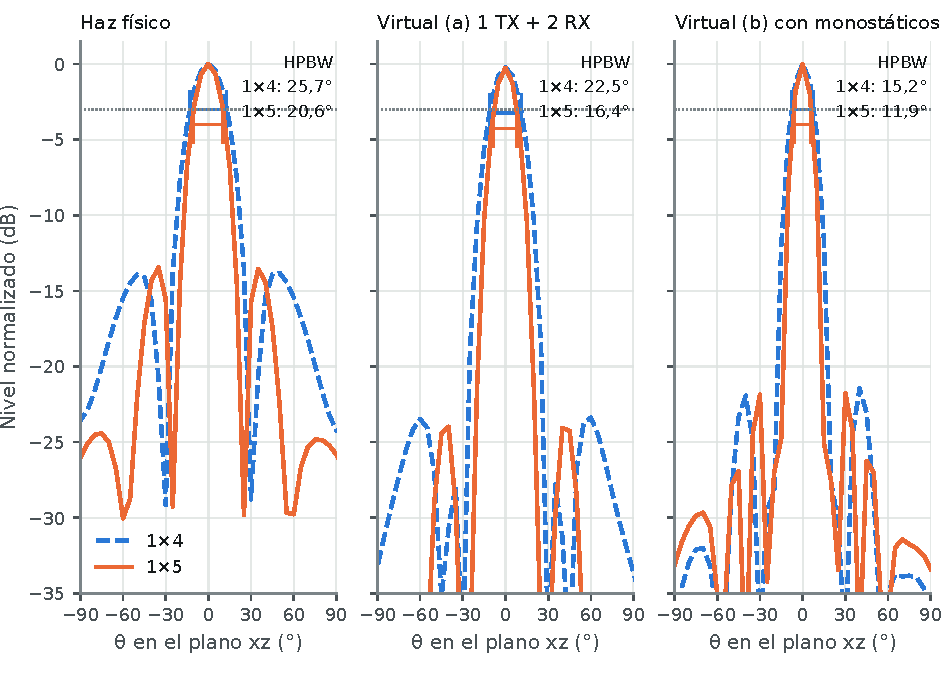
\includegraphics[width=0.85\textwidth]{../figures/arr_1x4_vs_1x5.pdf}
    \caption{Cortes $xz$ normalizados de los arrays 1$\times$4 y 1$\times$5 de P01\_MS2 a \SI{18.2}{mm} y a la frecuencia central: array físico, virtual solo biestático (a) y virtual con monostáticos (b). Fuente: diagramas embebidos exportados de HFSS.}
    \label{fig:arr_1x4_1x5_cortes}
\end{figure}

\begin{figure}[H]
    \centering
    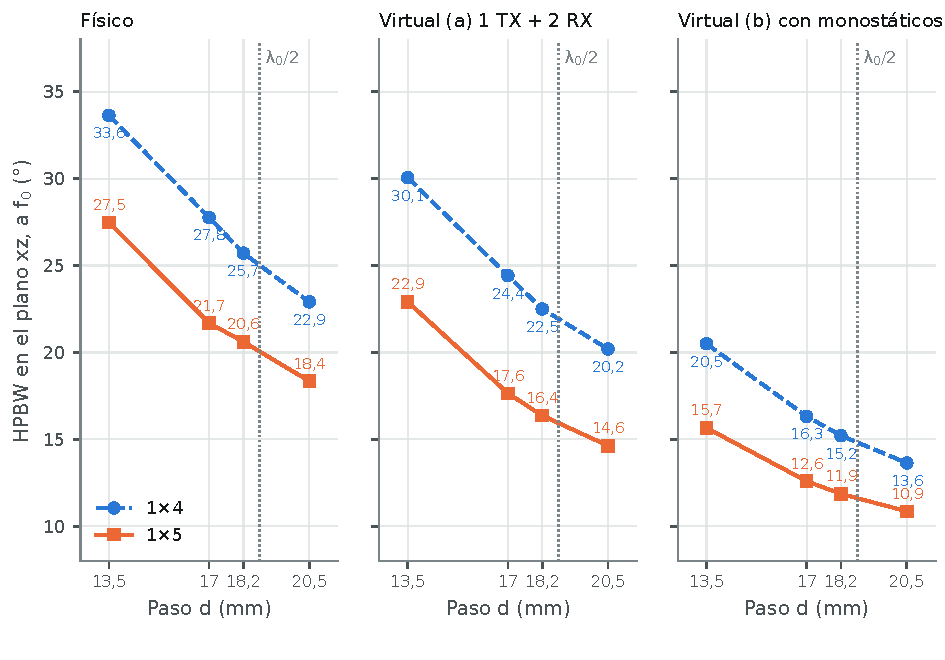
\includegraphics[width=0.85\textwidth]{../figures/arr_barrido_paso_1x4_1x5.pdf}
    \caption{HPBW físico y virtual en el plano $xz$ frente al paso $d$ para los arrays 1$\times$4 y 1$\times$5 de P01\_MS2 a la frecuencia central. La línea punteada es $\lambda_0/2$ (\SI{18.8}{mm}). Fuente: diagramas embebidos exportados de HFSS.}
    \label{fig:arr_1x4_1x5_paso}
\end{figure}

\subsection{Radar con pares monostáticos y biestáticos}\label{sec:mono_bi}
Hasta aquí el array virtual se ha calculado con la secuencia de un transmisor y dos receptores. Si el
SoC tiene un puerto de transmisión-recepción además del puerto solo de recepción, el elemento que
transmite también puede recibir, y aparecen pares monostáticos. Se comparan los dos casos con los
mismos diagramas embebidos de US3\_PS6\_4 y el mismo paso de \SI{18.2}{mm}.

El efecto de los pares monostáticos es geométrico.  Los pares monoestáticos sitúan el punto virtual en
el propio elemento transmisor, $v = x_t$, es decir, en múltiplos de $d$, mientras que los
biestáticos caen en el punto medio. Con cinco elementos, el conjunto de posiciones pasa de siete a
nueve, la extensión de $3d$ a $4d$ y la apertura eléctrica equivalente de $6d$ a $8d$. La Figura~\ref{fig:mono_bi_pos} muestra las posiciones y sus
multiplicidades.  El caso (b) necesita menos adquisiciones (20 en lugar de 30) para cubrir esa apertura.

\begin{figure}[H]
    \centering
    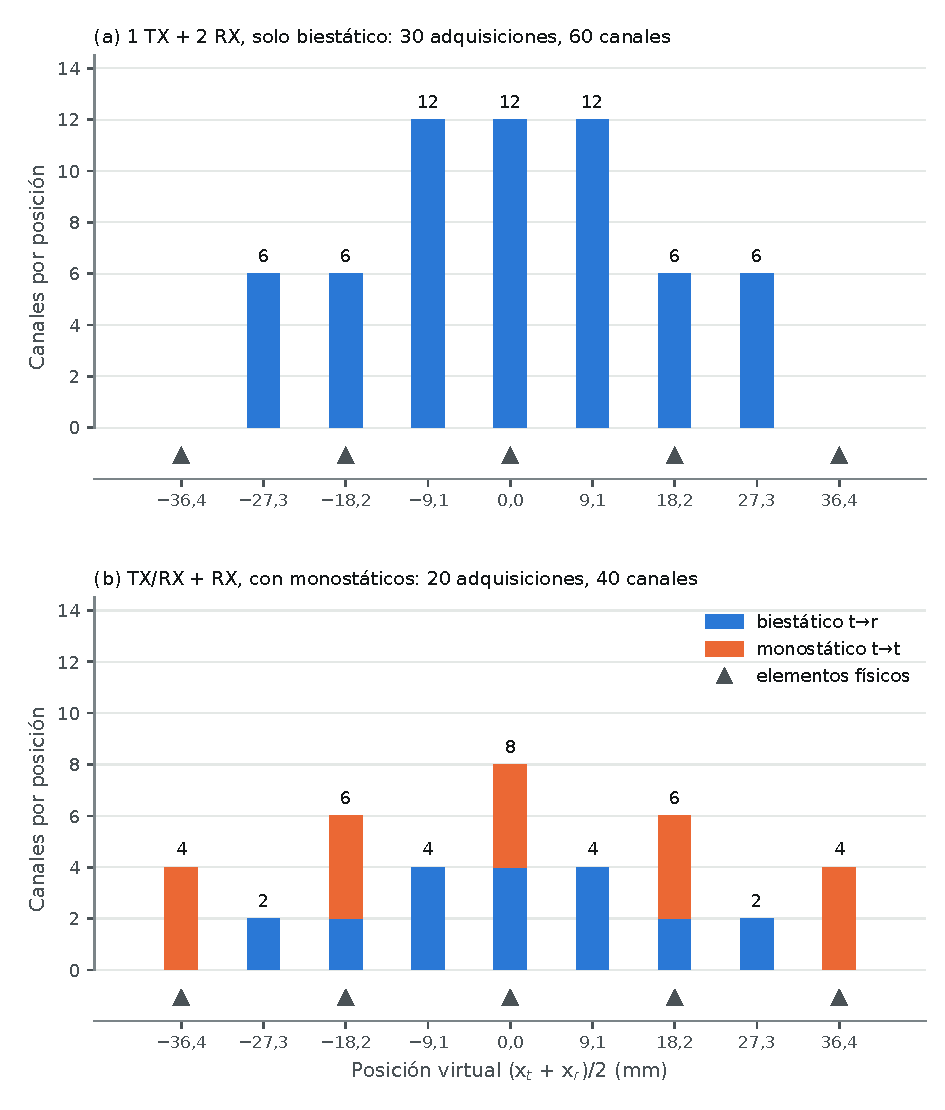
\includegraphics[width=0.85\textwidth]{../figures/arr_mono_bi_posiciones.pdf}
    \caption{Posiciones virtuales y multiplicidades del array 1$\times$5 con paso de \SI{18.2}{mm}:
    (a) solo biestáticos, un transmisor y dos receptores; (b) con pares monostáticos, puerto TX/RX y
    puerto solo RX. Las posiciones dependen solo del paso y del número de elementos, así que son las
    mismas en US3\_PS4\_2\_1 y en US3\_PS6\_4. Fuente: análisis de HFSS (\texttt{array\_virtual\_monostatic\_d18p2.json}, US3\_PS6\_4).}
    \label{fig:mono_bi_pos}
\end{figure}

La Figura~\ref{fig:mono_bi_cortes} y la Tabla~\ref{tab:mono_bi} recogen los resultados. El HPBW a
broadside baja de \SI{16.3}{\degree} a \SI{11.8}{\degree}, y apuntando a \SI{30}{\degree} de
\SI{18.8}{\degree} a \SI{13.8}{\degree}. El precio es un lóbulo secundario más alto. En broadside
sube de \SI{-24.4}{dB} a \SI{-22.1}{dB}, y a \SI{30}{\degree} llega a \SI{-8.2}{dB}, en la dirección de
\SI{-30}{\degree}. El análisis
lo atribuye a la periodicidad $2d$ de los pesos del canal monoestático y biestático. Ese lóbulo
reduce el margen frente a objetivos fuertes fuera del eje.

\begin{figure}[H]
    \centering
    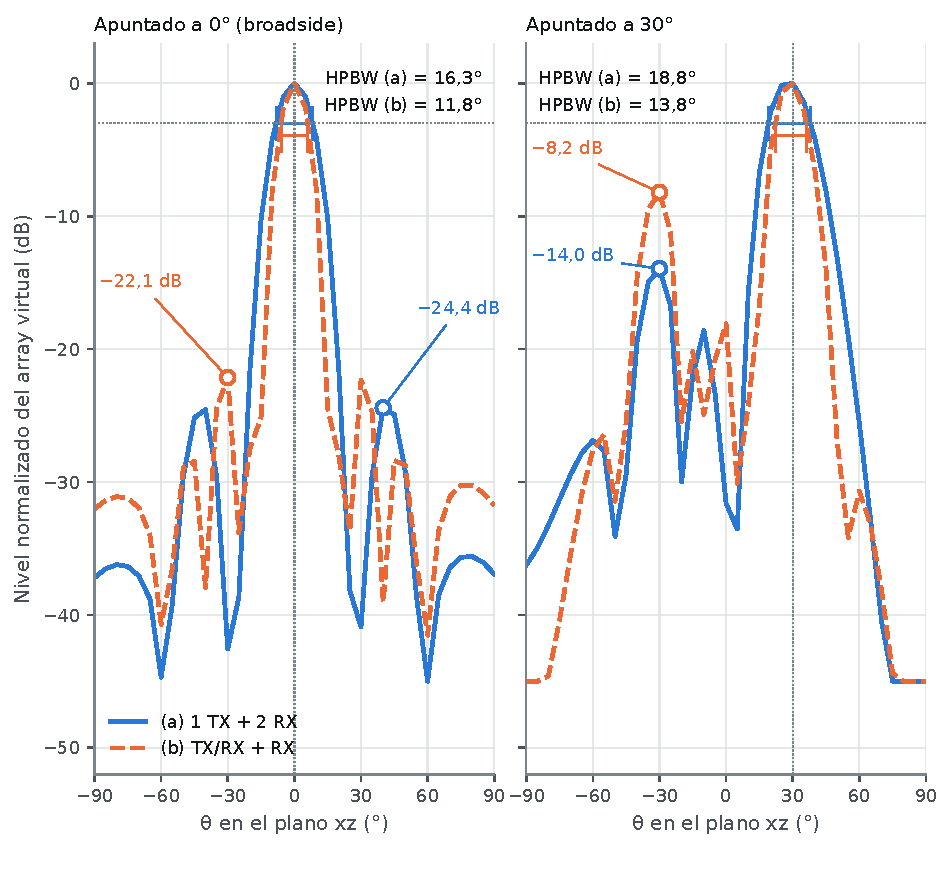
\includegraphics[width=0.85\textwidth]{../figures/arr_mono_bi_cortes_PS6_4.pdf}
    \caption{Cortes $xz$ del array virtual en broadside y apuntando a \SI{30}{\degree}, para (a) solo
    biestático y (b) con monostáticos, con HPBW de \SI{16.3}{\degree} a \SI{11.8}{\degree} en broadside y de \SI{18.8}{\degree} a
    \SI{13.8}{\degree} a \SI{30}{\degree}, con los lóbulos laterales marcados. Fuente: análisis de
    HFSS del array 1$\times$5 de US3\_PS6\_4 (\SI{18.2}{mm}, frecuencia central).}
    \label{fig:mono_bi_cortes}
\end{figure}

\begin{table}[H]
    \centering
    \caption{Comparación del array virtual de cinco elementos con paso de \SI{18.2}{mm}, a la frecuencia
    central. Son resultados del modelo guía: campo ideal radiado, sin la fuga entre los puertos TX y RX.}
    \label{tab:mono_bi}
    \begin{tabularx}{\textwidth}{X c c}
        \toprule
        Magnitud & (a) Solo biestático & (b) Con monostáticos \\
        \midrule
        Adquisiciones / canales & 30 / 60 & 20 / 40 \\
        Posiciones virtuales & 7 & 9 \\
        Extensión de las posiciones & $3d$ & $4d$ \\
        Apertura eléctrica equivalente & $6d$ & $8d$ \\
        HPBW, broadside (\si{\degree}) & $16{,}3$ & $11{,}8$ \\
        HPBW, $15\si{\degree}$ (\si{\degree}) & $17{,}2$ & $12{,}3$ \\
        HPBW, $30\si{\degree}$ (\si{\degree}) & $18{,}8$ & $13{,}8$ \\
        Lóbulo secundario más alto, broadside (\si{dB}) & $-24{,}4$ & $-22{,}1$ \\
        Lóbulo secundario más alto, $30\si{\degree}$ (\si{dB}) & $-14{,}0$ & $-8{,}2$ \\
        \bottomrule
    \end{tabularx}
\end{table}

Desde el punto de vista del SoC, el caso (b) tiene ventajas claras: más apertura y más resolución
con menos adquisiciones. Tiene también inconvenientes que no están en el modelo. El primero es la
fuga entre el puerto TX y el puerto RX del mismo puerto de transmisión-recepción, que es la limitación
más fuerte de un radar monoestático y no se modela aquí. El segundo es la reflexión de ese puerto, que
también queda fuera. El tercero es el lóbulo secundario más alto, que obliga a comprobar el margen en
las direcciones de interés. Por eso el caso (b) debe leerse como el canal radiado ideal, y no como una
predicción de la respuesta del radar.

\subsection{Rendimiento del sistema de agentes}\label{sec:rendimiento_agentes}
La campaña de diseño se ejecutó con el sistema de agentes descrito en la Sección~\ref{sec:metodologia}.
Las transcripciones de la sesión registran 76 tareas de subagentes a lo largo de la campaña.
La Tabla~\ref{tab:uso_agentes} las agrupa por rol con sus tokens, sus llamadas a herramientas y su
duración, y la Figura~\ref{fig:ag_subagentes} muestra la misma distribución.

\begin{table}[H]
    \centering
    \caption{Tareas de subagentes por rol, según las transcripciones
    de la sesión.}
    \label{tab:uso_agentes}
    \begin{tabularx}{\textwidth}{X c c c c}
        \toprule
        Rol & Tareas & Tokens & Llamadas & Minutos \\
        \midrule
        Validador & 31 & 2\,231\,858 & 558 & 85,7 \\
        Diseñador RF & 18 & 1\,550\,028 & 363 & 100,9 \\
        Especialista EM & 17 & 2\,235\,351 & 521 & 95,1 \\
        Generador de gráficas & 5 & 597\,385 & 250 & 31,3 \\
        Revisor de diseño & 3 & 473\,768 & 74 & 27,6 \\
        Auditor de código & 2 & 154\,345 & 32 & 4,0 \\
        \midrule
        Total & 76 & 7\,242\,735 & 1\,798 & 344,6 \\
        \bottomrule
    \end{tabularx}
\end{table}

\begin{figure}[H]
    \centering
    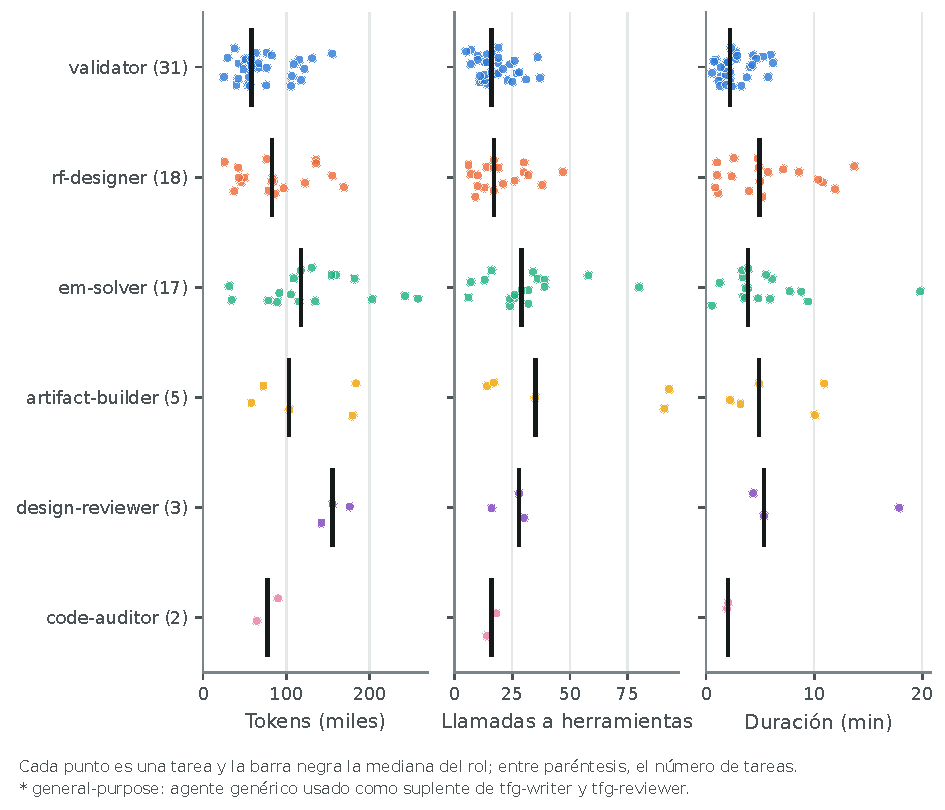
\includegraphics[width=0.85\textwidth]{../figures/ag_uso_subagentes.pdf}
    \caption{Uso de los subagentes agrupado por rol: tokens, llamadas a herramientas y duración de cada
    tarea. Fuente: transcripción de la sesión (bloques de uso de las notificaciones de subagentes).}
    \label{fig:ag_subagentes}
\end{figure}

Los tokens miden coste, no calidad. Lo que aportó valor a la campaña fue la auditoría independiente,
que frenó conclusiones erróneas antes de que llegaran a la memoria. De los 37 informes con veredicto
del auditor, 24 concluyen «aprobar con reservas» y 13, «OK con observaciones». No hubo ningún bloqueo
total. Sí hubo un bloqueo parcial temprano, sobre una configuración de puerto microstrip, que se
corrigió después. Veinte informes enumeran entre dos y nueve reservas (Figura~\ref{fig:ag_auditorias}). Algunos ejemplos concretos:
\begin{itemize}
    \item en la simulación base de US3\_PS4\_2\_1, el auditor independiente comprobó que algunas líneas de malla
    pedidas se fundían con otras, de modo que la malla efectiva no era la descrita;
    \item en la simulación de US3\_PS6\_3 se comprobó que su malla no era comparable con la de
    US3\_PS6, aunque la nota del fichero de variante hablaba de un solo cambio de línea;
    \item en la simulación fina de US3\_PS6\_4, el criterio de energía se cumplió en un valle de la
    envolvente; al recortar el \SI{30}{\percent} final del registro del puerto, $|\Gamma|$ cambió menos de $0{,}006$.
\end{itemize}

\begin{figure}[H]
    \centering
    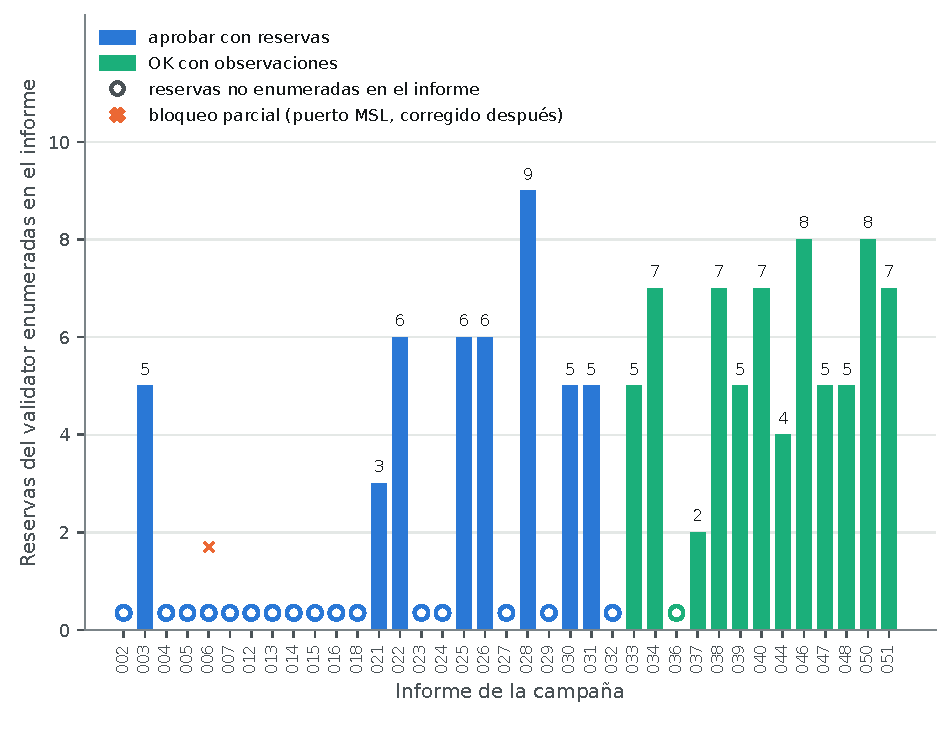
\includegraphics[width=0.85\textwidth]{../figures/ag_auditorias.pdf}
    \caption{Veredicto de las auditorías independientes de las simulaciones de openEMS (37 informes) y
    número de reservas registradas. Fuente: informes de auditoría de las simulaciones del repositorio.}
    \label{fig:ag_auditorias}
\end{figure}

Las simulaciones FDTD también se midieron. Las 30 simulaciones de openEMS de la campaña sumaron unas
\SI{6.7}{h} de tiempo de pared, entre \SI{1.6}{min} y \SI{51.1}{min}, este último para la malla fina de US3\_PS4\_2\_1.
La malla base de la familia US3\_PS tardó entre unos \SI{620}{s} y \SI{915}{s} de solver, con dos
hilos de cálculo, y las mallas finas de US3\_PS4\_2\_1 y US3\_PS6\_4 unos \SI{3000}{s}, con en torno a
\SI{1}{GiB} de memoria. La Figura~\ref{fig:ag_tiempos} muestra el tiempo de cada simulación.

\begin{figure}[H]
    \centering
    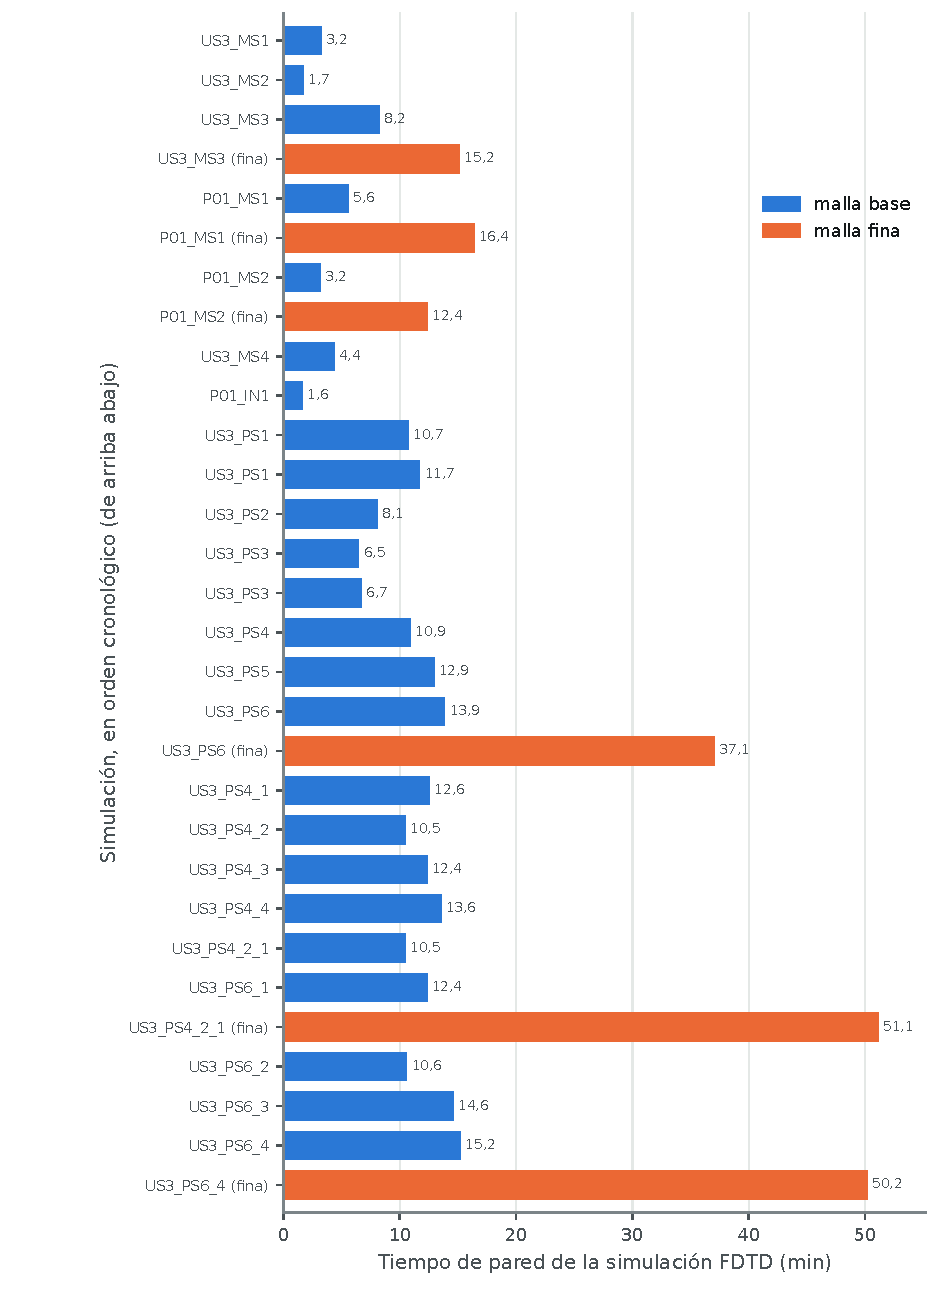
\includegraphics[width=0.85\textwidth]{../figures/ag_tiempos_fdtd.pdf}
    \caption{Tiempo de pared de cada una de las 30 simulaciones de openEMS de la campaña, en orden cronológico, para la
    malla base y la fina. Fuente: \texttt{campaign\_state.json} y \texttt{em/*/run\_numeric.json}.}
    \label{fig:ag_tiempos}
\end{figure}

Por último, la evaluación de modelos de lenguaje que se hizo sobre las primeras invocaciones se resume
en la Figura~\ref{fig:ag_tiers}. Mide tokens de salida, una magnitud distinta del recuento total de la
Tabla~\ref{tab:uso_agentes}.

\begin{figure}[H]
    \centering
    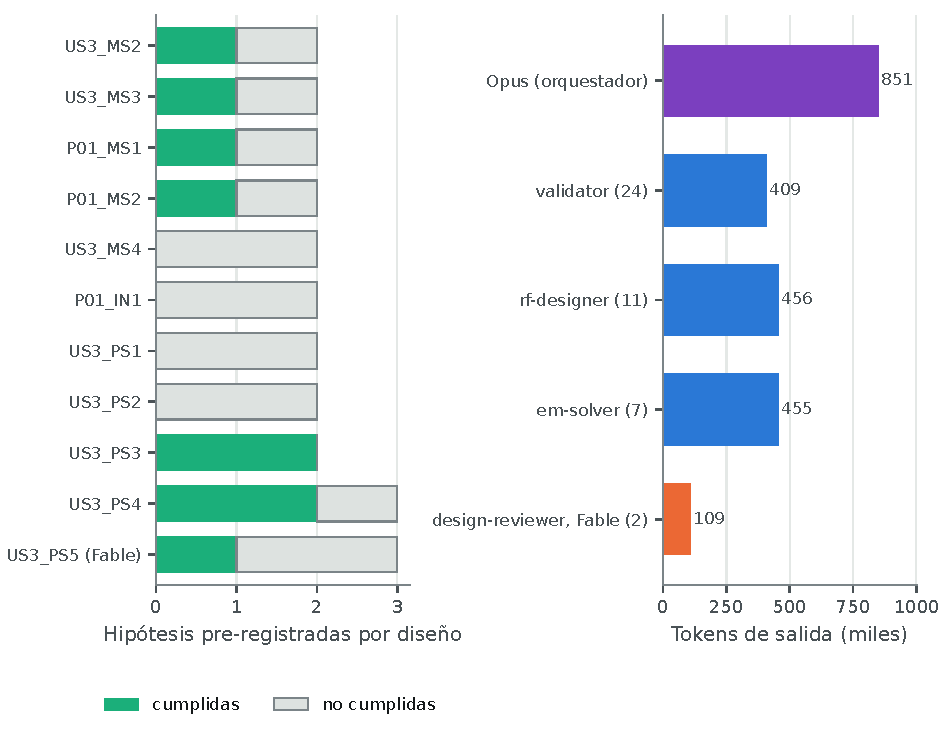
\includegraphics[width=0.9\textwidth]{../figures/ag_tiers.pdf}
    \caption{Izquierda: hipótesis pre-registradas cumplidas por diseño (9 de 24). Derecha: tokens de salida
    por rol en las 44 primeras invocaciones analizadas en la evaluación de modelos, a mitad de la campaña. Son tokens de salida, distintos del recuento total de la Tabla~\ref{tab:uso_agentes}.}
    \label{fig:ag_tiers}
\end{figure}

\subsection{Validación frente a objetivos}\label{sec:validacion}
La Tabla~\ref{tab:objetivos} compara los resultados con los objetivos del TFE. Se indica también el
estado de evidencia de cada resultado.

\begin{table}[H]
    \centering
    \caption{Cumplimiento de los objetivos según los datos disponibles.}
    \label{tab:objetivos}
    \begin{tabularx}{\textwidth}{>{\raggedright\arraybackslash}p{0.22\textwidth} X >{\raggedright\arraybackslash}p{0.22\textwidth}}
        \toprule
        Objetivo & Resultado & Estado \\
        \midrule
        $|S_{11}| \le \SI{-10}{dB}$ en todo el canal & US3\_PS6\_4 lo cumple en openEMS con dos mallas ($-10{,}92$ y $-11{,}24$\,\si{dB}). En HFSS, con puerto concentrado, su peor punto es $-9{,}82$\,\si{dB}, a $0{,}18$\,\si{dB} del objetivo y dentro de la incertidumbre de convergencia: no se cumple ni se descarta. US3\_PS4\_2\_1 lo cumple en HFSS en el límite ($-10{,}00$\,\si{dB}). US3\_PS6 no lo cumple ($-8{,}72$\,\si{dB} en HFSS). & \texttt{EM\_SIMULATED} (openEMS y HFSS) \\
        Eficiencia y ganancia & US3\_PS6\_4 tiene $\eta_\mathrm{rad}$ de $0{,}65$ a $0{,}71$ en openEMS y de $0{,}74$ a $0{,}78$ en HFSS, con ganancia realizada en broadside de $4{,}4$ a $5{,}0$\,\si{dBi} en HFSS. US3\_PS4\_2\_1 cae a $0{,}32$ en HFSS. & \texttt{HFSS\_VALIDATED} para la radiación, con la reserva del puerto \\
        Rizado del retardo de grupo radiado & Diagnóstico: US3\_PS6\_4 tiene unos \SI{18}{ps} en HFSS (entre \SI{15}{ps} y \SI{32}{ps} en openEMS); US3\_PS6 unos \SI{20}{ps} en HFSS; US3\_PS4\_2\_1 unos \SI{664}{ps} en HFSS. & Diagnóstico \\
        Resolución angular del array virtual & HPBW de \SI{16.3}{\degree} (caso a) y \SI{11.8}{\degree} (caso b) con US3\_PS6\_4 a \SI{18.2}{mm} (US3\_PS4\_2\_1: \SI{16.4}{\degree} y \SI{11.9}{\degree}). Referencia: \SI{24.0}{\degree}. & Modelo guía, \texttt{EM\_SIMULATED} \\
        Sin lóbulos de rejilla en el sector de interés & Con \SI{18.2}{mm}, $d \le \lambda/2$ en todo el canal (criterio analítico); el análisis no detecta lóbulos de rejilla en las configuraciones (a) y (b) al apuntar a \SI{0}{\degree}, \SI{15}{\degree} y \SI{30}{\degree}. Con pares monostáticos, la periodicidad $2d$ de los pesos produce un cuasi lóbulo de rejilla de unos \SI{-8}{dB} al apuntar a \SI{30}{\degree}. & Criterio analítico y \texttt{EM\_SIMULATED} \\
        \bottomrule
    \end{tabularx}
\end{table}

En resumen, el objetivo de adaptación en todo el canal se alcanza en openEMS con US3\_PS6\_4 y, en el límite, en HFSS con US3\_PS4\_2\_1. En HFSS, US3\_PS6\_4 queda a \SI{0.18}{dB} del objetivo, y su cumplimiento no se puede afirmar ni descartar con la convergencia alcanzada. El objetivo de eficiencia y de rizado se alcanza con US3\_PS6\_4 en openEMS y en HFSS. La resolución angular del array virtual mejora con respecto a la referencia en el modelo guía, pero el resultado de array no está validado: los arrays de P01\_MS2, US3\_PS4\_2\_1, US3\_PS6 y US3\_PS6\_4 son \texttt{EM\_SIMULATED}, con puerto concentrado y sin contraste con \textit{wave port}. Ningún resultado de esta memoria es una medida.

\section{Conclusiones}\label{sec:conclusiones}
\subsection{Logros alcanzados}
El trabajo ha producido un elemento radiante para el canal 9 de IEEE 802.15.4z que cubre la banda de \SI{499.2}{MHz} con $|S_{11}| \le \SI{-10}{dB}$ en las dos mallas de openEMS. El diseño con mejor radiación de la campaña, US3\_PS6\_4, es un parche con ranura en U y un parásito enterrado. En HFSS, con puerto concentrado, su peor punto es de \SI{-9.82}{dB}, en el borde superior del canal, y el \SI{96.4}{\percent} del canal queda por debajo de \SI{-10}{dB}: el cumplimiento total no queda demostrado ni refutado, y no se declara como candidato final. Como radiador, sus eficiencias están entre $0{,}74$ y $0{,}78$, su ganancia realizada en broadside entre \SI{4.4}{dBi} y \SI{5.0}{dBi}, y su rizado del retardo de grupo radiado es de unos \SI{18}{ps}. Su estado de evidencia es \texttt{EM\_SIMULATED} para la adaptación, en openEMS y en HFSS, y \texttt{HFSS\_VALIDATED} para la radiación, con la reserva del puerto concentrado. Por el camino se planteó como hipótesis una «adaptación por pérdidas» en las versiones de parásito, que el criterio de adaptación por sí solo no detecta y que no está confirmada.

Se ha construido además un flujo de simulación y análisis con agentes de inteligencia artificial, en
el que cada resultado se registra con su estado de evidencia y su procedencia, y en el que las
auditorías independientes corrigieron afirmaciones antes de que llegaran a la memoria. Ese flujo
permitió pasar de un parche de una sola capa a un candidato que cubre todo el canal en openEMS.

Por último, el array de cinco elementos con paso de \SI{18.2}{mm} produce, en el modelo guía, un array virtual con HPBW de \SI{16.3}{\degree} o \SI{11.8}{\degree} con US3\_PS6\_4, según se usen solo pares biestáticos o también monostáticos, prácticamente los mismos que con US3\_PS4\_2\_1 y US3\_PS6; su adaptación pasiva es de \SI{-10.73}{dB} en el peor puerto, pero la reflexión activa a \SI{0}{\degree} queda en \SI{-9.23}{dB} y solo cumple \SI{-10}{dB} a \SI{15}{\degree}. Con P01\_MS2, el quinto elemento estrecha frente al array de cuatro elementos el haz virtual un \SI{27}{\percent} en el caso biestático y un \SI{22}{\percent} con monostáticos, sin empeorar de forma apreciable la adaptación pasiva ni el acoplo entre vecinos, aunque la reflexión activa a \SI{0}{\degree} empeora de \SI{-10.0}{dB} a \SI{-9.3}{dB}. Esa es la mejora de resolución angular que motivó el TFE, aunque todavía no es un resultado validado: la adaptación de los arrays es \texttt{EM\_SIMULATED}.

\subsection{Limitaciones}
Las limitaciones condicionan el alcance de los resultados y conviene enumerarlas:
\begin{itemize}
    \item El sustrato es un FR-4 provisional, con $\varepsilon_r = 4{,}4$ y $\tan\delta = 0{,}017$, sin
    caracterizar. Las pérdidas dieléctricas, que controlan la eficiencia, dependen de esos valores.
    \item No hay medidas. Ningún diseño está en estado \texttt{MEASURED}, y la comparación con el
    prototipo queda pendiente.
    \item La alimentación es un puerto concentrado de \SI{50}{\ohm} en el borde de la placa, sin
    conector SMA ni sonda. El plano de referencia es el del puerto, y el escalón de la línea de
    \SI{50}{\ohm} junto al puerto no se ha validado con un \textit{wave port}.
    \item Dos mallas no son convergencia. Las diferencias entre ellas acotan la sensibilidad, pero no
    demuestran el valor verdadero. US3\_PS4\_2\_1 tiene un $|\Delta\Gamma|$ de $0{,}20$, lo que obliga a
    tratar su adaptación en el canal con cautela.
    \item Los barridos paramétricos (Optimetrics) de los arrays de US3 no están todos completamente convergidos. El de US3\_PS6\_4 converge en sus 11 pasos con $\Delta S < 0{,}01$, aunque de forma justa a \SI{18.2}{mm}. En US3\_PS4\_2\_1, el criterio de $\Delta S \le 0{,}01$ en dos pasadas se cumple en 15 de los 16 pasos, pero el de \SI{18.2}{mm} tiene menos refinamiento que sus vecinos y la solución es una continuación de la del barrido anterior, de modo que $\Delta S$ no acota el error; en US3\_PS6, la convergencia solo se documenta en tres de los 16 pasos. Los barridos de P01\_MS2 convergen en los 16 pasos, pero con un criterio de $\Delta S \le 0{,}02$ en una pasada, menos estricto, y el registro de convergencia del array de cinco elementos procede de una nueva exportación de la misma solución.
    \item La adaptación de HFSS se obtiene con un puerto concentrado y sin contraste con un \textit{wave port}, por eso se clasifica como \texttt{EM\_SIMULATED}. El peor punto de US3\_PS6\_4 en HFSS (\SI{-9.82}{dB}) queda a \SI{0.18}{dB} del objetivo, dentro de la incertidumbre de convergencia. El array de cinco elementos de US3\_PS6\_4 se simuló en HFSS con 11 separaciones y su adaptación también es \texttt{EM\_SIMULATED}; a \SI{18.2}{mm}, la reflexión activa a \SI{0}{\degree} no alcanza \SI{-10}{dB} (\SI{-9.23}{dB}).
    \item El modelo del array es un modelo guía con suma coherente y pesos uniformes. No incluye la
    fuga TX-RX del puerto TX/RX ni la reflexión de ese puerto, y el caso monostático es el canal radiado ideal.
\end{itemize}

\subsection{Trabajo futuro}\label{sec:futuro}
Quedan varias líneas abiertas, por orden de prioridad:
\begin{itemize}
    \item Contrastar la adaptación de US3\_PS6\_4 en HFSS con un \textit{wave port} y de-embedding en el mismo plano de referencia, y comprobar si el borde superior de la banda queda por debajo de \SI{-10}{dB}. Ese resultado decide si la adaptación pasa de \texttt{EM\_SIMULATED} a \texttt{HFSS\_VALIDATED}, y debe hacerse antes de cualquier refinamiento.
    \item Refinar la convergencia del array de US3\_PS6\_4 en el paso de \SI{18.2}{mm}, donde el $\Delta S$ final es de $0{,}0095$, y valorar un paso algo mayor (a \SI{19}{mm} la reflexión activa a \SI{0}{\degree} ya cumple \SI{-10}{dB}) frente a la aparición de lóbulos de rejilla al apuntar.
    \item Fabricar un prototipo de US3\_PS6\_4 y medir $|S_{11}|$, la eficiencia y el retardo de grupo,
    para cerrar el ciclo de evidencia.
    \item Probar un sustrato de bajas pérdidas, que separe la pérdida dieléctrica de la metálica y confirme
    o descarte la hipótesis de adaptación por pérdidas.
    \item Incorporar el procesado de señal en el canal de cada configuración MIMO, con el SoC real, una vez
    confirmada la topología de sus puertos.
\end{itemize}

\newpage
\begin{thebibliography}{99}
\addcontentsline{toc}{section}{Bibliografía}
\bibitem{ieee802154z2020}
IEEE Computer Society, \textit{IEEE Std 802.15.4z-2020: IEEE Standard for Low-Rate Wireless Networks--Amendment 1: Enhanced Ultra Wideband (UWB) Physical Layers (PHYs) and Associated Ranging Techniques}, IEEE, 2020.

\bibitem{coppens2022uwb}
D. Coppens, A. Shahid, S. Lemey, B. Van Herbruggen, C. Marshall, and E. De Poorter, ``An Overview of Ultra-WideBand (UWB) Standards and Organizations (IEEE 802.15.4, FiRa, Apple): Interoperability Aspects and Future Research Directions,'' \textit{IEEE Access}, vol. 10, pp. 70219--70241, 2022.

\bibitem{cheraghinia2024uwbradar}
M. Cheraghinia, A. Shahid, S. Luchie, G. J. Gordebeke, O. Caytan, J. Fontaine, B. Van Herbruggen, S. Lemey, and E. De Poorter, ``A Comprehensive Overview on UWB Radar: Applications, Standards, Signal Processing Techniques, Datasets, Radio Chips, Trends and Future Research Directions,'' arXiv preprint arXiv:2402.05649, 2024.

\bibitem{carretero2027vpa}
L. Carretero López, C. Urquizar Herrera, and M. Sáez Rodríguez, ``Design of Virtual Phased Arrays for Ultrawideband Localization,'' manuscrito enviado a EuCAP 2027.

\bibitem{fcc2002uwb}
Federal Communications Commission, ``Revision of Part 15 of the Commission's Rules Regarding Ultra-Wideband Transmission Systems,'' First Report and Order, ET Docket 98-153, 2002.

\bibitem{wiesbeck2009uwb}
W. Wiesbeck, G. Adamiuk, and C. Sturm, ``Basic Properties and Design Principles of UWB Antennas,'' \textit{Proceedings of the IEEE}, vol. 97, no. 2, pp. 372--385, 2009.

\bibitem{pozar2012microwave}
D. M. Pozar, \textit{Microwave Engineering}, 4th ed., Wiley, 2012.

\bibitem{fano1950bode}
R. M. Fano, ``Theoretical Limitations on the Broadband Matching of Arbitrary Impedances,'' \textit{Journal of the Franklin Institute}, vol. 249, no. 1, pp. 57--83, 1950.

\bibitem{balanis2016antenna}
C. A. Balanis, \textit{Antenna Theory: Analysis and Design}, 4th ed., Wiley, 2016.

\bibitem{huynh1995uslot}
T. Huynh and K.-F. Lee, ``Single-Layer Single-Patch Wideband Microstrip Antenna,'' \textit{Electronics Letters}, vol. 31, no. 16, pp. 1310--1312, 1995.

\bibitem{vantrees2002array}
H. L. Van Trees, \textit{Optimum Array Processing: Part IV of Detection, Estimation, and Modulation Theory}, Wiley-Interscience, 2002.

\bibitem{mailloux2005phased}
R. J. Mailloux, \textit{Phased Array Antenna Handbook}, 2nd ed., Artech House, 2005.

\bibitem{pozar1994active}
D. M. Pozar, ``The Active Element Pattern,'' \textit{IEEE Transactions on Antennas and Propagation}, vol. 42, no. 8, pp. 1176--1178, 1994.

\bibitem{li2007mimo}
J. Li and P. Stoica, ``MIMO Radar with Colocated Antennas,'' \textit{IEEE Signal Processing Magazine}, vol. 24, no. 5, pp. 106--114, 2007.

\bibitem{yee1966numerical}
K. S. Yee, ``Numerical Solution of Initial Boundary Value Problems Involving Maxwell's Equations in Isotropic Media,'' \textit{IEEE Transactions on Antennas and Propagation}, vol. 14, no. 3, pp. 302--307, 1966.

\bibitem{taflove2005fdtd}
A. Taflove and S. C. Hagness, \textit{Computational Electrodynamics: The Finite-Difference Time-Domain Method}, 3rd ed., Artech House, 2005.

\bibitem{liebig2013openems}
T. Liebig, A. Rennings, S. Held, and D. Erni, ``openEMS: A Free and Open Source Equivalent-Circuit (EC) FDTD Simulation Platform Supporting Cylindrical Coordinates Suitable for the Analysis of Traveling Wave MRI Applications,'' \textit{International Journal of Numerical Modelling: Electronic Networks, Devices and Fields}, vol. 26, no. 6, pp. 680--696, 2013.

\bibitem{jin2014fem}
J.-M. Jin, \textit{The Finite Element Method in Electromagnetics}, 3rd ed., Wiley-IEEE Press, 2014.

\bibitem{haupt1995genetic}
R. L. Haupt, ``An Introduction to Genetic Algorithms for Electromagnetics,'' \textit{IEEE Antennas and Propagation Magazine}, vol. 37, no. 2, pp. 7--15, 1995.

\bibitem{robinson2004pso}
J. Robinson and Y. Rahmat-Samii, ``Particle Swarm Optimization in Electromagnetics,'' \textit{IEEE Transactions on Antennas and Propagation}, vol. 52, no. 2, pp. 397--407, 2004.

\bibitem{yao2023react}
S. Yao, J. Zhao, D. Yu, N. Du, I. Shafran, K. Narasimhan, and Y. Cao, ``ReAct: Synergizing Reasoning and Acting in Language Models,'' in \textit{Proc. International Conference on Learning Representations (ICLR)}, 2023.

\bibitem{anthropic2024agents}
E. Schluntz and B. Zhang, ``Building Effective Agents,'' Anthropic, dic. 2024. [En línea]. Disponible: \url{https://www.anthropic.com/engineering/building-effective-agents}

\end{thebibliography}


\appendix
\section{Repositorio del proyecto}\label{app:repositorio}
El código, los datos de simulación, los informes de la campaña y esta memoria están en el repositorio
\url{https://github.com/luiscarlop/uwb-antenna-lab}. La rama \texttt{master} contiene la versión
de referencia. La estructura principal es la siguiente:

{\small
\begin{verbatim}
uwb-antenna-lab/
|-- README.md             Descripción del proyecto y guía de reproducción
|-- antenna_design/       Trabajo principal del TFE
|   |-- variants/         Definición geométrica de cada diseño (JSON)
|   |-- em/               Simulaciones FDTD en openEMS, una carpeta por ejecución
|   |-- hfss/
|   |   |-- build/        Scripts de AEDT que construyen cada modelo
|   |   |-- export/       Scripts de exportación de parámetros S y campos
|   |   |-- analysis/     Análisis de elementos y arrays (array virtual MIMO)
|   |   `-- results/      Resultados exportados de HFSS por diseño
|   |-- analysis/         Análisis comunes de las simulaciones
|   |-- reports/          Informes de cada ronda y de cada exportación de HFSS
|   |-- artifacts/        Fuentes de la página de resumen visual
|   |-- tests/            Pruebas unitarias
|   `-- campaign_state.json, automation_policy.json
|-- latex_memoir/         Fuentes LaTeX y figuras de esta memoria
|-- .claude/, CLAUDE.md   Configuración del sistema de agentes (Claude Code)
`-- .codex/, AGENTS.md    Configuración equivalente para Codex
\end{verbatim}
}

Cada simulación de openEMS guarda en su carpeta la malla efectiva, los registros del solver, el
$S_{11}$ complejo, los resultados de campo lejano y los ficheros de origen con su huella SHA-256.
Los resultados de HFSS incluyen, para cada diseño y cada paso del array, la matriz $S$ en formato
Touchstone, el registro de convergencia adaptativa y los diagramas de campo lejano exportados.
Las carpetas \texttt{legacy\_*} dentro de \texttt{hfss/results/} conservan exportaciones superadas
por trazabilidad. El estado de evidencia de cada diseño y su procedencia se recogen en
\texttt{campaign\_state.json} y en los informes de \texttt{reports/}.

% Anexos ocultos: no se usan por ahora. Descomentar para recuperarlos.
% \section{Código extendido}\label{app:codigo}
% En este anexo se podrá incluir código adicional que sea demasiado extenso para el cuerpo principal de la memoria.

% \section{Datasheets}\label{app:datasheets}
% En este anexo se podrán recopilar hojas de características de componentes, antenas, placas o equipos utilizados.

% \section{Cálculos largos}\label{app:calculos}
% En este anexo se podrán desarrollar deducciones matemáticas o cálculos que complementen las secciones principales.

% \section{Manual de usuario}\label{app:manual_usuario}
% En este anexo se podrán documentar instrucciones de uso, ejecución o reproducción de los experimentos.

% \section{Configuraciones}\label{app:configuraciones}
% En este anexo se podrán registrar configuraciones de simulación, parámetros de medida y ajustes relevantes.

% \section{Resultados completos}\label{app:resultados_completos}
% En este anexo se podrán incluir tablas o gráficas completas que respalden el análisis resumido en el capítulo de resultados.

%%%%%%%%%%%%%%%%%%%%%%%%%%%%%%%%%%%%%%%%%%%%%%%%%%%%%%%%%%%%%%%%%%%%%%%%%%
\end{document}
